\documentclass[journal,onecolumn, 10pt,draftclsnofoot]{IEEEtran}
\IEEEoverridecommandlockouts

\usepackage{amsmath,amssymb,amsfonts,amsthm}
% \usepackage{textcomp}
% \usepackage{abstract}
% \usepackage{algorithm,algorithmicx}
\usepackage[ruled,vlined]{algorithm2e}
\usepackage[noend]{algpseudocode} 
\usepackage{graphicx}
\usepackage{makecell}
\usepackage{epstopdf}
\usepackage{xcolor}
\usepackage{cite}
\usepackage{latexsym}
\usepackage{float}
\usepackage{multirow}
% \usepackage{txfonts}
% \usepackage{mathptmx}
\usepackage{mathrsfs}
\usepackage{exscale}
\usepackage{relsize}
\usepackage{enumerate}
\usepackage{soul}
\usepackage{tikz,pgfplots}
\pgfplotsset{compat=1.18}
\usepackage{flowchart}
\usepackage{tabularx}
\usepackage{booktabs}
\usepackage[switch]{lineno}
\usepackage{bbding}
\usepackage{stfloats}
\usepackage{arydshln}
% \usepackage{caption}
\setlength{\abovecaptionskip}{.cm}
\setlength{\belowcaptionskip}{-0.5cm}
\usepackage[bookmarks=false]{hyperref}
\usepackage{subcaption}
\usepackage{minted}

% Configure minted for better code display
\setminted[python]{
    fontsize=\footnotesize,
    linenos=true,
    breaklines=true,
    bgcolor=gray!10,
    frame=lines,
    framesep=2mm
}
\definecolor{lavendergray}{rgb}{0.77, 0.76, 0.82}
\def\BibTeX{{\rm B\kern-.05em{\sc i\kern-.025em b}\kern-.08em
T\kern-.1667em\lower.7ex\hbox{E}\kern-.125emX}}

\usepackage{fancyhdr}  
\usepackage{setspace}
\pagestyle{fancy}      
\fancyhf{}             
\fancyhead[C]{HE-BCI Analysis Project Report}
\fancyfoot[C]{\thepage}
\setlength{\headheight}{13.92pt}


\captionsetup{justification=centering, font=small}

\begin{document}

\begin{titlepage}
    \thispagestyle{fancy} 
    \vspace*{5cm} 
    \fancyfoot{}
    \begin{center}
        \setstretch{2}
        {\LARGE \textbf{Analysing Higher Education Business and Community Interaction (HE-BCI) Data for Durham University and the North East of England}} \\[1cm]
        {
        {Student Name [2025]} \\ {Department of xxx, xxx University} \\ 
        \href{https://github.com/xvsfvv/HE-BCI-Analysis-Project}{GitHub Repository: https://github.com/xvsfvv/HE-BCI-Analysis-Project}} \\[1cm]
        
    \end{center}
    
    \vfill  


\end{titlepage}

\newpage
\thispagestyle{fancy} 
\vspace{-0.9cm}

\begin{abstract}
    The Higher Education Business and Community Interaction (HE-BCI) survey, conducted by HESA (2024) \cite{hesa_he_bci_2024}, serves as a crucial tool for assessing the scope and impact of knowledge exchange activities within UK universities. This comprehensive survey collects annual financial and output data on collaborative research, consultancy services, IP commercialization, CPD courses, continuing education, public lectures, exhibitions, and cultural activities that connect universities with businesses, public institutions, and broader communities. This project conducts a detailed analysis of HE-BCI data for Durham University and the North East of England region, focusing on the period from 2014/15 to 2023/24. The analysis covers five key areas: Income Analysis, Intellectual Property Analysis, Public Engagement Analysis, Regional and Specialization Analysis, and Trend Prediction Analysis. The project employs a comprehensive analytical framework to examine the HE-BCI data from multiple perspectives, providing strategic insights for enhancing knowledge exchange strategies, driving economic growth and innovation, and assessing Durham University's performance against regional and national benchmarks.
\end{abstract}
\begin{IEEEkeywords}
Higher Education, Business and Community Interaction, Knowledge Exchange, Durham University, North East England, Data Analysis, Strategic Planning
\end{IEEEkeywords}

\section{Introduction}

\subsection{Background}

The Higher Education Business and Community Interaction (HE-BCI) survey, established by HESA (2024) \cite{hesa_he_bci_2024} in 1999, serves as a crucial tool for assessing the scope and impact of knowledge exchange activities within UK universities. This foundation builds upon the work of Etzkowitz and Leydesdorff (2000) \cite{etzkowitz2000dynamics} and Perkmann et al. (2013) \cite{perkmann2013academic}. This comprehensive survey collects annual financial and output data on collaborative research, consultancy services, IP commercialization, CPD courses, continuing education, public lectures, exhibitions, and cultural activities that connect universities with businesses, public institutions, and broader communities. These activities play a crucial role in fostering collaboration between universities and external partners, contributing to economic growth, innovation, and societal development.

\subsection{Project Objectives}

This project conducts a detailed analysis of HE-BCI data for Durham University and the North East of England region, focusing on the period from 2014/15 to 2023/24. The primary objectives are to:
\begin{itemize}
    \item Evaluate the effectiveness and impact of knowledge exchange activities
    \item Identify regional patterns and trends in university-business interactions
    \item Assess Durham University's performance against regional and national benchmarks
    \item Provide strategic insights for enhancing knowledge exchange strategies
\end{itemize}

\subsection{Scope of Analysis}

My analysis covers five key areas. Income Analysis focuses on various revenue streams, including income from collaborative research, business services, continuing professional development (CPD) and continuing education, as well as regeneration and development projects. Intellectual Property Analysis examines IP disclosures and patents, licensing activities, IP-related income, and the performance of spin-off companies. Public Engagement Analysis evaluates social and cultural events, community engagement initiatives, and public participation metrics. Regional and Specialization Analysis explores university rankings across different indicators, identifies specialization trends using the Herfindahl-Hirschman Index (HHI), and assesses competitive positioning by region. Finally, Trend Prediction Analysis provides forecasts of future developments, highlights areas of potential growth or decline, and offers insights to support strategic planning.

Note: Formula for HHI (Herfindahl-Hirschman Index), developed by Hirschman (1945) \cite{hirschman1945national} and Herfindahl (1950) \cite{herfindahl1950concentration}, given a university's income or activity data across multiple categories $x_{i 1}, x_{i 2}, \ldots, x_{i n}$, where $i$ denotes the university, $n$ is the number of categories (e.g., research fields, business service types, etc.). The HHI is calculated as,

1) Calculate the share of each category: $s_{i j}=\frac{x_{i j}}{\sum_{j=1}^n x_{i j}}$. Where $s_{i j}$ is the proportion of university $i$ 's total value in category $j$.

2) Compute the HHI index: $\mathrm{HHI}_i=\sum_{j=1}^n s_{i j}^2$.

3) HHI close to 1: High specialization (most activity concentrated in a few categories). HHI close to 0: High diversification (activity distributed across many categories)

\section{Literature Review}

\subsection{University-Industry Collaboration and Knowledge Exchange}

The theoretical foundation for university-industry collaboration stems from the Triple Helix model, proposed by Etzkowitz and Leydesdorff (2000) \cite{etzkowitz2000dynamics}, which conceptualizes the dynamic interactions between universities, industry, and government as drivers of innovation and economic development. This framework has evolved to encompass various forms of knowledge exchange, from formal contractual arrangements to informal networking and collaborative research initiatives, as documented by Perkmann et al. (2013) \cite{perkmann2013academic}.

Recent research has highlighted the complexity of measuring knowledge exchange performance, particularly in the UK context. Rossi and Rosli (2015) \cite{rossi2015indicators} emphasize that traditional performance indicators often privilege certain activities, particularly intellectual property commercialization, while overlooking other valuable forms of engagement such as consultancy, continuing professional development, and public engagement. Their analysis of UK HE-BCI data reveals that universities differ significantly in their knowledge transfer objectives and profiles, with implications for funding allocation and institutional strategy. This finding directly informs our analysis of Durham University's diverse income streams and the need to evaluate performance beyond simple financial metrics.

The efficiency of university-industry collaboration has been a focus of recent empirical work. Bertoletti and Johnes (2021) \cite{bertoletti2021efficiency} employ data envelopment analysis to assess the relative efficiency of UK higher education institutions in contract research activities. Their findings reveal substantial variation in efficiency across universities, with larger and research-intensive institutions generally achieving higher performance. However, they note that factors beyond institutional size, including management practices, governance structures, and strategic orientation toward industry engagement, are crucial determinants of success. This research provides the theoretical foundation for our efficiency analysis in Section~\ref{sec:performance-efficiency}, where we examine Durham University's performance relative to regional peers using similar efficiency metrics.

\subsection{Forms and Evolution of Knowledge Exchange Activities}

The landscape of university knowledge exchange has evolved significantly, encompassing both formal and informal mechanisms. Zhou and Baines (2024) \cite{zhou2024extent} examine the interaction between formal knowledge exchange activities (such as patents, licensing, and spin-offs) and informal activities (including consultancy, collaborative research, and continuing professional development) using UK HE-BCI survey data. Their analysis reveals that informal activities often serve as enablers or precursors to commercialization outcomes, suggesting that universities should maintain a balanced portfolio of engagement strategies. This finding directly supports our analytical approach in Sections~\ref{sec:income-analysis} and~\ref{sec:ip-analysis}, where we examine both IP commercialization and business services to understand Durham University's comprehensive knowledge exchange portfolio.

Open innovation has emerged as a key concept in understanding university-industry collaboration. Gustina et al. (2024) \cite{gustina2024open} provide a comprehensive review of research trends and practices in open innovation between universities and industries. Their bibliometric analysis identifies an evolution from early focus on technology transfer to more recent emphasis on innovation ecosystems, governance mechanisms, and stakeholder dynamics. The study highlights the importance of trust building, explicit collaboration norms, and resource commitment in successful partnerships. This research framework informs our regional analysis in Section~\ref{sec:regional-analysis}, where we assess Durham University's positioning within the North East innovation ecosystem and its collaborative relationships with regional partners.

\subsection{Regional Development and Entrepreneurship Education}

The role of universities in regional development has gained increasing attention, particularly in the context of devolution and regional disparities. Bozward et al. (2021) \cite{bozward2021impact} investigate the impact of enterprise and entrepreneurship education on regional development across the UK, combining HE-BCI data with economic statistics. Their findings reveal significant regional variations in graduate start-up generation, business survival rates, and employment creation, with universities in economically disadvantaged regions often playing a disproportionately important role in stimulating local entrepreneurship. This research directly informs our regional analysis in Section~\ref{sec:regional-analysis}, where we examine Durham University's performance within the North East context and assess its contribution to regional economic development through knowledge exchange activities.

The development of enterprise and entrepreneurship education within higher education institutions has been documented by Rae et al. (2012) \cite{rae2012enterprise}, who conducted a national survey of English HEIs. Their research shows a marked expansion of enterprise provision between 2006 and 2010, with 93\% of institutions supporting student enterprise and graduate entrepreneurship. However, they also identify challenges in sustaining provision, particularly in the face of reduced public funding and the need to demonstrate value creation from entrepreneurial activities. These findings provide context for our analysis of Durham University's CPD and continuing education performance in Section~\ref{sec:income-analysis}, where we examine the university's engagement in professional development and its financial sustainability in this area.

\subsection{Policy Context and Institutional Performance}

The policy context for university knowledge exchange in the UK has evolved significantly over the past two decades. Zhang (2018) \cite{zhang2018theory} provides a longitudinal study of university knowledge exchange policy and practice, examining the period from 2003/04 to 2012/13. The study confirms the important roles of institutional characteristics (established vs. new universities) and locational factors (competitive vs. uncompetitive regions) in determining knowledge exchange performance. However, Zhang argues that current policy approaches fail to adequately consider the heterogeneity of the higher education sector, potentially disadvantaging institutions with different strategic orientations or regional contexts. This research provides important context for our analysis of Durham University's performance relative to other institutions in Section~\ref{sec:regional-analysis}, where we examine how institutional characteristics and regional positioning influence knowledge exchange outcomes.

The literature consistently emphasizes the need for more nuanced approaches to performance measurement and funding allocation. Rossi and Rosli (2015) \cite{rossi2015indicators} argue that relying on narrow, income-focused indicators risks rewarding scale and profitability rather than true performance or impact. They advocate for more comprehensive sets of indicators that capture the diversity of knowledge exchange activities and their qualitative aspects, including interaction quality, stakeholder satisfaction, and long-term benefits. This perspective directly supports our multi-dimensional analytical framework in Section~\ref{sec:performance-efficiency}, where we employ efficiency metrics and risk analysis to provide a more comprehensive assessment of Durham University's performance beyond simple income measures.

\subsection{Methodological Approaches and Analytical Frameworks}

The methodological approaches employed in this analysis build upon established frameworks in higher education research and institutional analysis. The use of efficiency metrics, including data envelopment analysis, introduced by Charnes et al. (1978) \cite{charnes1978measuring} and extended by Banker et al. (1984) \cite{banker1984models}, has become standard in assessing institutional performance. Johnes (2006) \cite{johnes2006data} provides a comprehensive overview of DEA applications in higher education, emphasizing the importance of appropriate input-output specifications and the interpretation of efficiency scores. This methodological foundation directly supports our efficiency analysis in Section~\ref{sec:performance-efficiency}, where we employ similar efficiency metrics to assess Durham University's performance relative to regional peers.

Risk and resilience analysis in higher education draws from portfolio theory, originated from Markowitz (1952) \cite{markowitz1952portfolio} and Sharpe (1964) \cite{sharpe1964capital}, with institutions seeking to balance income diversification against specialization benefits. The coefficient of variation and Herfindahl-Hirschman Index provide complementary measures of financial stability and concentration risk, enabling institutions to assess their vulnerability to external shocks and policy changes. These analytical tools are central to our resilience and risk analysis in Section~\ref{sec:resilience-risk}, where we examine Durham University's financial stability and income diversification patterns using the same theoretical framework.

\subsection{Research Gaps and Future Directions}

Despite the extensive literature on university knowledge exchange, several research gaps remain. The interaction between formal and informal knowledge exchange activities requires further investigation, particularly in understanding how different institutional contexts and strategic orientations influence these relationships. The role of regional factors in shaping knowledge exchange outcomes also warrants deeper analysis, especially in understanding how universities can contribute to regional innovation ecosystems while maintaining their academic mission.

The literature also highlights the need for more sophisticated approaches to performance measurement that go beyond simple financial metrics. Future research should explore the development of multidimensional performance indicators that capture both quantitative outputs and qualitative impacts, enabling more nuanced assessment of institutional contributions to knowledge exchange and regional development.

\section{Methodology}
\label{sec:methodology}

\subsection{Analytical Framework}

This project employs a comprehensive analytical framework, developed by PACEC and Centre for Business Research (2016) \cite{pacec2016state}, designed to systematically evaluate knowledge exchange performance across multiple dimensions. The framework integrates descriptive, comparative, efficiency, risk, and predictive analyses to provide a holistic understanding of institutional performance and strategic positioning. The analytical approach follows a logical progression,
\begin{enumerate}
    \item \textbf{Descriptive Analysis}: Establishes baseline performance metrics and identifies patterns across institutions and time periods
    \item \textbf{Comparative Analysis}: Benchmarks Durham University against regional peers and national standards
    \item \textbf{Efficiency Analysis}: Evaluates resource utilization and output generation effectiveness
    \item \textbf{Risk and Resilience Analysis}: Assesses financial stability and vulnerability to external shocks
    \item \textbf{Predictive Analysis}: Forecasts future trends and identifies strategic opportunities
\end{enumerate}

\subsection{Data Processing Methodology}

\subsubsection{Dataset Overview}
The HE-BCI dataset, compiled by HESA (2024) \cite{hesa_he_bci_2024}, consists of 10 detailed tables covering various aspects of university-business interactions from 2014/15 to 2023/24. The dataset tables are summarized in Table~\ref{tab:dataset-overview}.

\vspace{0.3cm}
\begin{table}[h]
\centering
\caption{HE-BCI Dataset Structure and Description}
\vspace{0.1cm}
\renewcommand{\arraystretch}{1.15}
\small
\begin{tabularx}{\textwidth}{|>{\raggedright\arraybackslash}p{3cm}
                                |>{\centering\arraybackslash}p{2cm}
                                |>{\raggedright\arraybackslash}p{5.2cm}
                                |>{\raggedright\arraybackslash}X|}
    \hline
    \textbf{Category} & \textbf{Table No.} & \textbf{Table Title} & \textbf{Breakdown Dimensions} \\
    \hline
    Collaborative Research and Business Services & Table 1 & Income from collaborative research involving public funding & Academic Year, Income Type, Public Funding Source, HE Provider \\
    \hline
    Collaborative Research and Business Services & Table 2a & Business and community services & Service Type, Academic Year, Organization Type, HE Provider \\
    \hline
    Collaborative Research and Business Services & Table 2b & Continuing Professional Development (CPD) and Continuing Education (CE) courses & Academic Year, HE Provider \\
    \hline
    Collaborative Research and Business Services & Table 3 & Income from regeneration and development programmes & Academic Year, Programme Type, HE Provider \\
    \hline
    Intellectual Property (IP) Analysis & Table 4a & IP disclosures and patents & Academic Year, Disclosure/Patent Type, HE Provider \\
    \hline
    Intellectual Property (IP) Analysis & Table 4b & License numbers & Academic Year, License Type, Organization Type, HE Provider \\
    \hline
    Intellectual Property (IP) Analysis & Table 4c & IP income by source & Academic Year, Income Source, Organization Type, HE Provider \\
    \hline
    Intellectual Property (IP) Analysis & Table 4d & Total IP income & Academic Year, HE Provider \\
    \hline
    Intellectual Property (IP) Analysis & Table 4e & Spin-out activities & Activity Type, Academic Year, Metric, HE Provider \\
    \hline
    Public Engagement & Table 5 & Social, community and cultural engagement events & Academic Year, Event Type, Event Nature, Attendee Numbers, Academic Staff Time (Days), HE Provider \\
    \hline
\end{tabularx}
\label{tab:dataset-overview}
\end{table}

\subsubsection{Data Structure and Quality Assessment}
Each table in the dataset follows a standardized structure. The first 11 rows contain metadata, including information about the location, time period, and data source. Row 12 presents the column headers, and the actual data begins from row 13. Across all tables, several columns are commonly included: UKPRN (the unique identifier for each institution), HE Provider (the name of the higher education institution), Country/Region of HE provider, and Academic Year.

The dataset covers the time span 2014/15 to 2023/24 (10 academic years) with 228 total institutions. The North East region institutions include Durham University, Newcastle University, University of Northumbria at Newcastle, The University of Sunderland, and Teesside University.

Several data quality issues were identified, primarily related to missing values across multiple tables. Figure~\ref{fig:missing-values} illustrates the missing value patterns across different tables for the dataset, showing the data completeness and quality issues that required systematic preprocessing.

\begin{figure}[h]
\centering
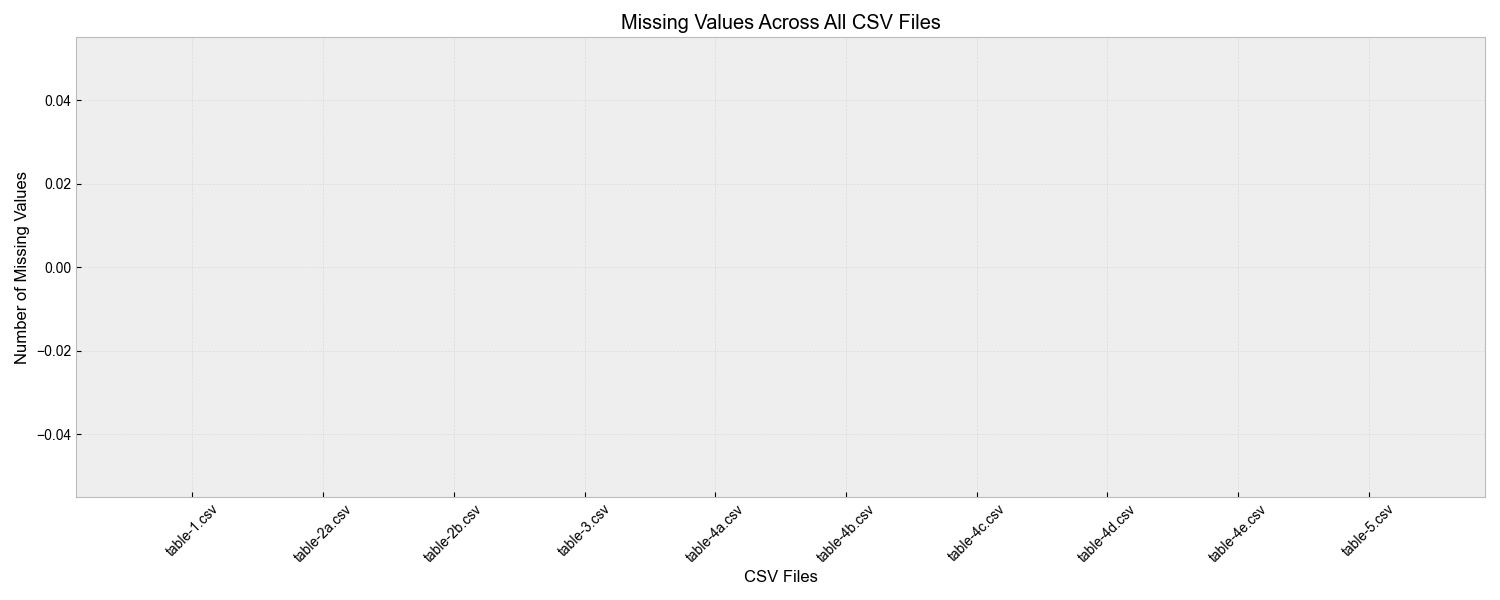
\includegraphics[width=0.8\textwidth]{Fig/figure1.missing_values_comparison.png}
\caption{Missing values across all tables}
\label{fig:missing-values}
\end{figure}

In the dataset: Table 1 contained 25 missing values in the Value column. Table 2a exhibited moderate data gaps, with 22,500 missing values in the Unit column and 12 missing values in the Number/Value column. Table 2b was largely complete, with 5 missing values in the Value column. Table 3 reported 1,452 missing values in the Value column. For the intellectual property data: Table 4a and Table 4b contained no missing values, while Table 4c had 9 missing values, Table 4d had 5 missing values, and Table 4e had 10 missing values in the Value column. Table 5, covering social and cultural engagement events, exhibited zero missing values.

Data consistency was maintained across all tables with consistent structure, standardized units (\textsterling 000s for financial data), and uniform institution identifiers.

\subsubsection{Data Preprocessing Strategy}
The HE-BCI dataset required systematic preprocessing to address data quality issues. Missing values were identified across multiple tables, with varying degrees of completeness. A consistent imputation strategy was implemented where missing values in income columns were replaced with zero, based on the assumption that unrecorded activity implies no financial engagement. Missing counts were similarly treated as zero, indicating no recorded activity. Inconsistent units were standardized to ensure comparability across institutions and time periods.

To address missing data across the HE-BCI tables, a consistent imputation strategy was applied. For all numeric columns such as Value and Number/Value, missing entries were replaced with zero, based on the assumption that no recorded activity or income implies zero engagement. This approach was applied to key tables, including Table 1 (Collaborative Research), Table 2a (Consultancy and Services), Table 2b (CPD and Education), Table 3 (Regeneration Income), and Tables 4c-4d (IP Income). Additionally, where the Unit column was incomplete, values were inferred based on the data type "\textsterling 000s" for financial amounts and "Count" for activity measures. This process reduced missingness and ensured consistency across years and institutions, supporting robust trend and comparative analysis.

This approach was chosen because HE-BCI data represents actual recorded activities, and missing entries typically indicate no activity rather than data collection errors. Several transformations were applied to enhance analytical capabilities, including time series conversion for trend analysis, institutional grouping for comparative analysis, and calculation of derived performance metrics such as efficiency ratios and volatility measures.

\subsection{Statistical Analysis Methods}

Basic descriptive statistics were computed for all key performance indicators, including central tendency measures (mean, median, and mode values for income and activity metrics), variability analysis (standard deviation, coefficient of variation, and range analysis), and distribution examination with outlier identification.

Efficiency was measured using output-to-input ratios, as developed by Charnes et al. (1978) \cite{charnes1978measuring} and Banker et al. (1984) \cite{banker1984models}, specifically income per academic staff day, $\text{Efficiency} = \frac{\text{Income}}{\text{Academic Staff Days}}$. This metric was chosen because it normalizes performance by resource input, enabling fair comparison across institutions of different sizes.

\subsubsection{Risk and Resilience Analysis}

Financial resilience was assessed using two complementary measures, Coefficient of Variation (CV), as developed by Pearson (1896) \cite{pearson1896contributions} and Fisher (1922) \cite{fisher1922mathematical},
\begin{equation}
\mathrm{CV} = \frac{\sigma}{\mu}
\end{equation}
where $\sigma$ is the standard deviation and $\mu$ is the mean income. The Herfindahl-Hirschman Index (HHI), as developed by Hirschman (1945) \cite{hirschman1945national} and Herfindahl (1950) \cite{herfindahl1950concentration},
\begin{equation}
\mathrm{HHI}_i = \sum_{j=1}^n s_{ij}^2
\end{equation}
where $s_{ij}$ is the proportion of university $i$'s total value in category $j$. The CV measures income volatility, while HHI measures income concentration. Lower CV indicates greater stability, and lower HHI indicates greater diversification.

\subsection{Predictive Modeling Approach}

Five distinct forecasting models were selected to capture different aspects of temporal patterns and uncertainty. Linear Regression captures long-term linear trends and provides interpretable coefficients for strategic planning. Exponential Smoothing, developed by Hyndman and Athanasopoulos (2018) \cite{hyndman2018forecasting}, adapts to recent changes and is robust to outliers, suitable for short-term forecasting. Random Forest, introduced by Breiman (2001) \cite{breiman2001random}, captures non-linear relationships and provides uncertainty estimates through ensemble methods. ARIMA models, developed by Box et al. (2015) \cite{box2015time}, autocorrelation and seasonal patterns, essential for time series with inherent dependencies. XGBoost, created by Chen and Guestrin (2016) \cite{chen2016xgboost}, handles complex interactions and provides high accuracy for non-linear trend patterns.

Models were evaluated using multiple criteria to ensure robust forecasting. Mean Absolute Error (MAE) measures average prediction error magnitude, Mean Absolute Percentage Error (MAPE) provides error relative to actual values, and R-squared ($R^2$) indicates proportion of variance explained by the model, as proposed by Hyndman and Koehler (2006) \cite{hyndman2006another}.

\subsection{Clustering Analysis}

K-means and hierarchical clustering, introduced by MacQueen (1967) \cite{macqueen1967methods} and Ward (1963) \cite{ward1963hierarchical} respectively, were applied to group institutions based on performance trajectories. Normalized performance indicators were derived from the five predictive models for feature engineering. Euclidean distance was used for K-means, while Ward's method was applied for hierarchical clustering. Silhouette analysis, developed by Rousseeuw (1987) \cite{rousseeuw1987silhouettes}, and elbow method, proposed by Thorndike (1953) \cite{thorndike1953belongs}, were used to determine optimal cluster numbers.

\subsection{Analytical Limitations and Assumptions}

Several limitations affect the analysis and should be considered when interpreting results. The time period is limited to 10 years (2014/15-2023/24), which may not capture long-term cycles. Focus on North East institutions limits generalizability to other regions, and some tables contain missing values, requiring assumptions for imputation.

Key assumptions underlying the analysis include zero imputation assuming no recorded activity equals no engagement, some models assuming linear relationships that may not hold for all metrics, and time series models assuming data properties remain constant over time.

The analysis acknowledges but does not explicitly model several external factors, including HE-BCI survey methodology and funding policy evolution, broader economic factors affecting university-business interactions, and COVID-19 pandemic effects on engagement patterns and data collection.


\section{Analysis \& Results}
\label{sec:analysis-results}

I employ a comprehensive analytical framework to examine the HE-BCI data from five distinct perspectives. The income analysis delves into the financial aspects of knowledge exchange activities, examining revenue streams from collaborative research, business services, and professional development programs. The intellectual property analysis focuses on the commercialization of university research outputs, tracking metrics such as patent filings, licensing activities, and spin-off company performance. The public engagement analysis evaluates the universities' social impact through various community and cultural activities, measuring both participation levels and academic staff involvement. The regional and specialization analysis provides a competitive landscape view, using ranking comparisons and the HHI (Herfindahl-Hirschman Index) to assess universities' positioning and focus areas within the North East region. Finally, the trend prediction analysis employs multiple forecasting models to project future developments in key metrics, offering strategic insights for long-term planning. Together, these five analytical dimensions provide a holistic understanding of the universities' knowledge exchange activities, their impact, and future potential.

\subsection{Exploratory Trend Analysis}

As part of initial data exploration, average values for each of the five North East institutions were plotted over time, combining indicators from all available tables. This multi-year trend analysis revealed several key insights: Newcastle University exhibited the highest and most stable average engagement values throughout most of the period, with a significant peak in 2018/19 and strong recovery post-COVID. Durham University displayed strong performance in earlier years (notably 2017/18-2018/19), followed by a dip and modest rebound in recent years. Teesside University maintained relatively consistent activity, showing growth in community-oriented indicators. Northumbria and Sunderland reported lower averages overall, but their patterns suggest gradual diversification and expansion in recent years. Figure~\ref{fig:institutions-trends} presents the average value trends for all five institutions across the 2014/15-2023/24 period. This chart highlights not only institutional differences in knowledge exchange volume, but also year-to-year volatility likely influenced by policy shifts, external funding availability, and the COVID-19 pandemic's disruption from 2019/20 onwards.

\begin{figure}[h]
\centering
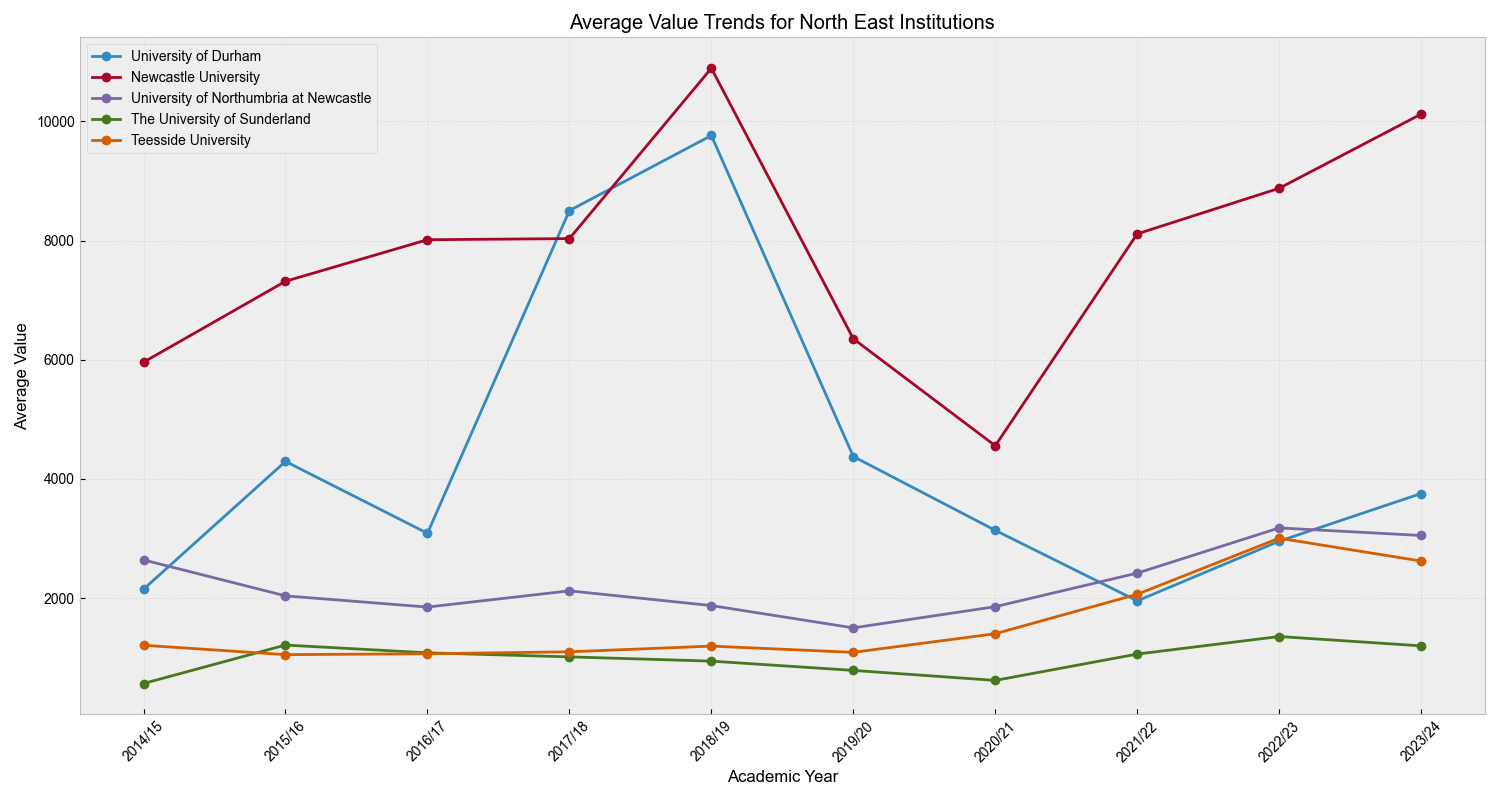
\includegraphics[width=0.8\textwidth]{Fig/figure2.ne_institutions_trends.png}
\caption{Average Value Trends for North East Institutions}
\label{fig:institutions-trends}
\end{figure}

\subsection{Income Analysis}
\label{sec:income-analysis}

\subsubsection{Collaborative Research Income}

Durham University's collaborative research income totaled \textsterling 216,850, with a substantial portion (\textsterling 66,123) coming from major public funders such as UKRI (excluding Research England), the Royal Society, and the British Academy. Additional sources included EU government funding (\textsterling 17,445), BEIS Research Councils (\textsterling 13,095), other UK government departments (\textsterling 7,273), and other smaller contributors (\textsterling 4,489).

The income structure shows that public funding accounted for \textsterling 173,280, supplemented by collaborative contributions of \textsterling 11,626 in cash and \textsterling 31,944 in kind. Compared to the previous year's total of \textsterling 206,006, this indicates a relatively stable financial input from both institutional and collaborative sources.

Durham University ranked 33rd out of 228 higher education institutions in the UK for collaborative research income, exceeding the national average by \textsterling 87,327, with the national average recorded at \textsterling 129,523. This ranking reflects Durham's strong national standing in securing competitive research funding. Within the North East region, Durham placed second in collaborative research income, behind Newcastle University (\textsterling 1,105,304), and significantly outperformed regional peers including Northumbria (\textsterling 134,470), Teesside (\textsterling 68,844), and Sunderland (\textsterling 2,744), demonstrating its leading role in regional research collaborations.

\begin{figure}[h]
\centering
\begin{subfigure}[b]{0.48\textwidth}
    \centering
    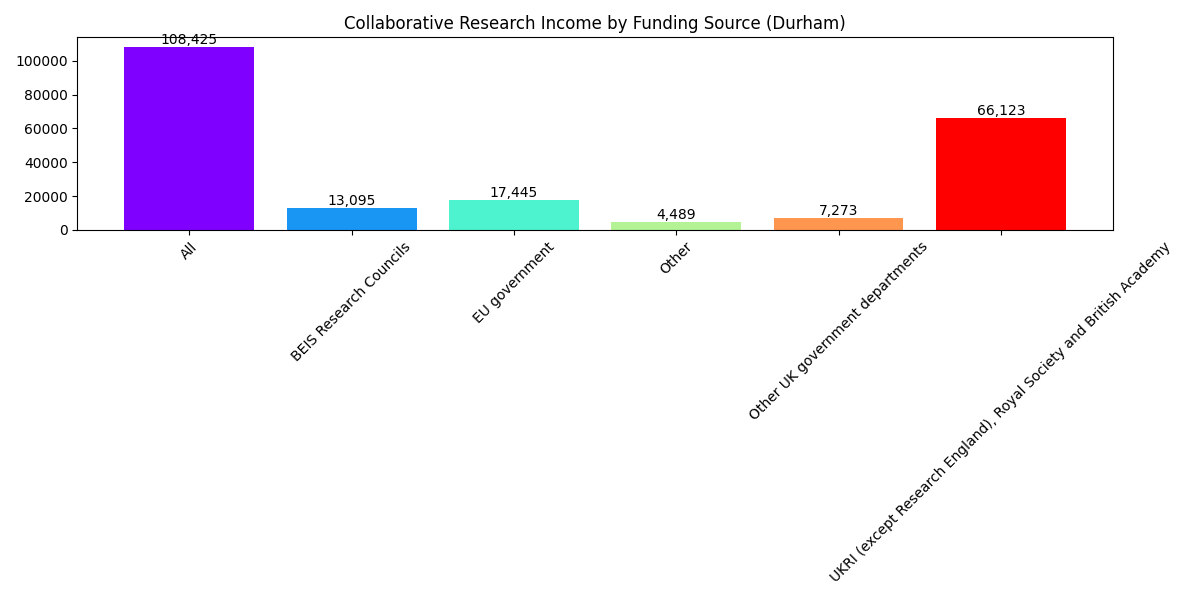
\includegraphics[width=\textwidth]{Fig/figure3.research_funding_source.png}
    \caption{Research funding source}
    \label{fig:research-funding}
\end{subfigure}
\hfill
\begin{subfigure}[b]{0.48\textwidth}
    \centering
    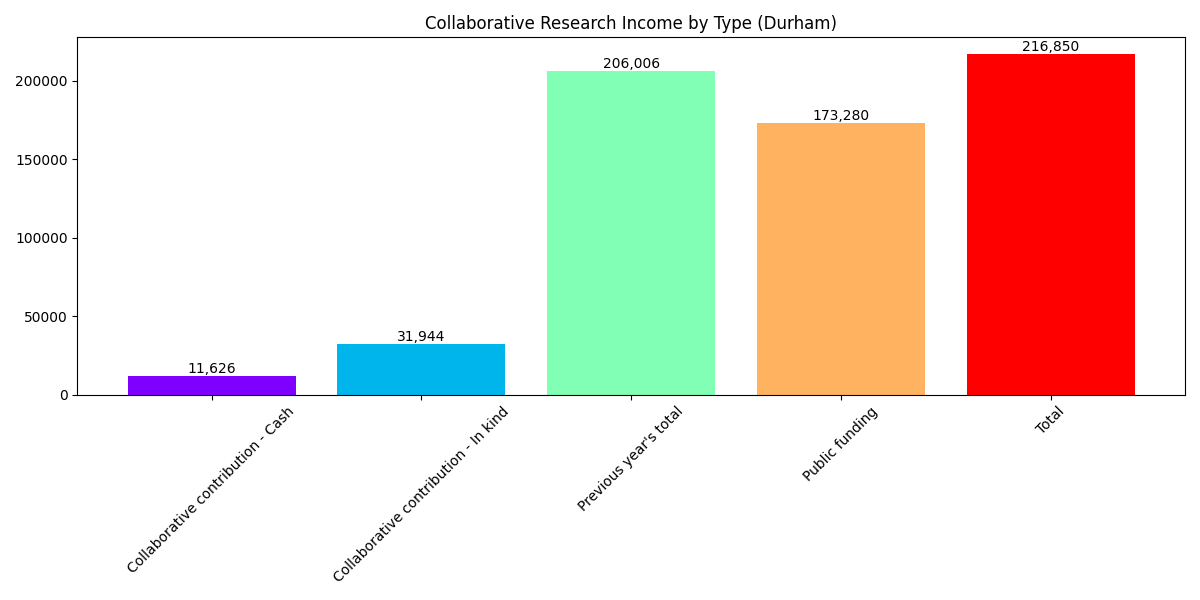
\includegraphics[width=\textwidth]{Fig/figure4.research_income_type.png}
    \caption{Research income type}
    \label{fig:research-income-type}
\end{subfigure}
\vspace{0.6cm}
\begin{subfigure}[b]{0.48\textwidth}
    \centering
    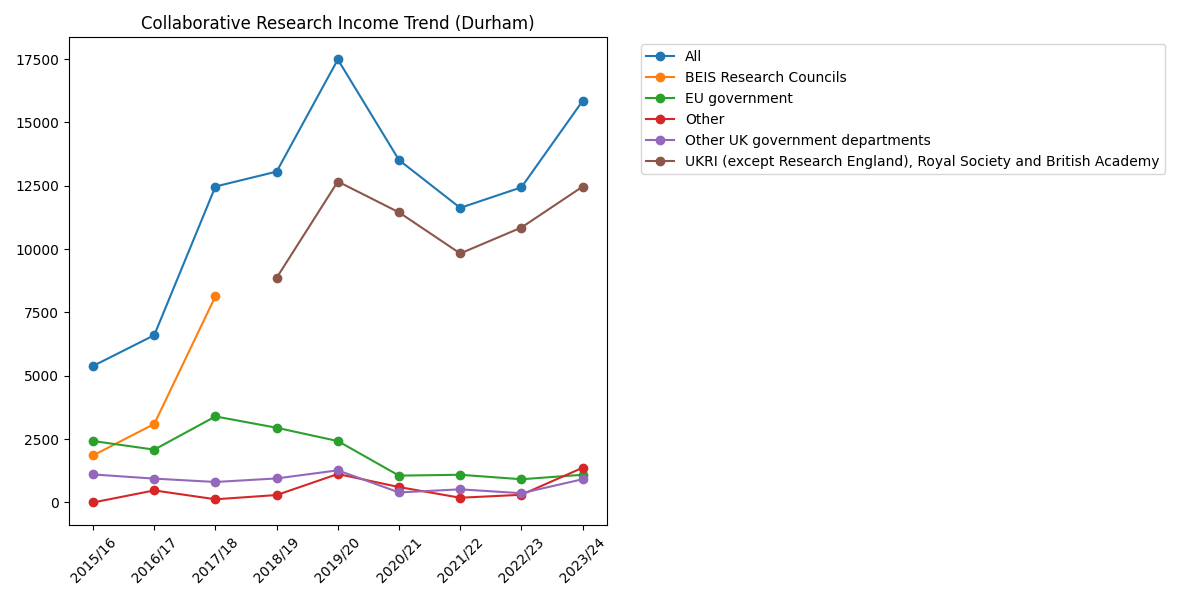
\includegraphics[width=\textwidth]{Fig/figure5.research_time_trend.png}
    \caption{Research time trend}
    \label{fig:research-time-trend}
\end{subfigure}
\hfill
\begin{subfigure}[b]{0.48\textwidth}
    \centering
    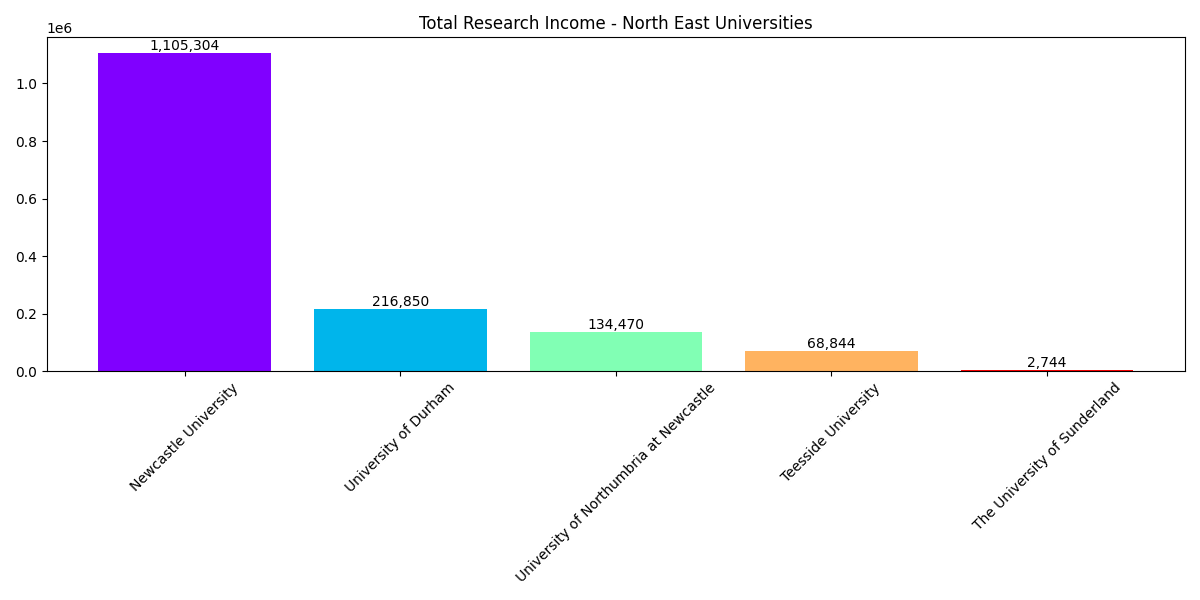
\includegraphics[width=\textwidth]{Fig/figure6.research_ne_comparison.png}
    \caption{Research NE comparison}
    \label{fig:research-ne-comparison}
\end{subfigure}
\caption{Research Income Analysis}
\label{fig:research-income-analysis}
\end{figure}

Durham University demonstrates strong research income performance, significantly outperforming the national average and maintaining a leading position in the North East region. The diverse funding sources and substantial collaborative contributions indicate robust research partnerships and effective knowledge exchange activities. Figures~\ref{fig:research-funding} through~\ref{fig:research-ne-comparison} provide comprehensive visualizations of Durham's research income patterns, funding sources, temporal trends, and regional positioning.

\subsubsection{Business Services}

Durham University generated a total of \textsterling 157,635 from business and community services, with income primarily derived from contract research (\textsterling 101,064 or 64.1\%), followed by consultancy services (\textsterling 44,671 or 28.3\%), and the use of facilities and equipment (\textsterling 11,900 or 7.5\%), indicating a well-balanced and diversified service portfolio.

A majority of business services income came from non-commercial organisations (\textsterling 94,773 or 60.1\%), followed by other commercial businesses (\textsterling 53,004 or 33.6\%) and small and medium-sized enterprises (SMEs) (\textsterling 9,858 or 6.3\%), suggesting that Durham has a strong client base in the public and non-profit sectors. In terms of service metrics, Durham provided \textsterling 157,635 worth of value-based services and \textsterling 103,120 worth of number-based services, indicating a balanced delivery of both qualitative and quantitative services in its business engagements.

Regionally, Durham ranked second in the North East for business service income, behind Newcastle University (\textsterling 347,009). Nationally, it was ranked 40th out of 228 universities, performing \textsterling 61,302 above the national average, which underscores its strong market presence and sector engagement.


\vspace{0.2cm}
\begin{table}[h]
\centering
\caption{Business Services Analysis - Durham University}
\vspace{0.1cm}
\resizebox{0.9\textwidth}{!}{%
\begin{tabular}{|l|l|l|r|r|}
\hline \textbf{Service Type} & \textbf{Organization Type} & \textbf{Value (\textsterling)} & \textbf{Percentage} & \textbf{Notes} \\
\hline \multirow{3}{*}{Contract Research} & Non-commercial organisations & 59,821 & 37.9\% & \multirow{3}{*}{Primary service (64.1\%)} \\
\cline{2-4}
& Other (non-SME) commercial & 37,536 & 23.8\% & \\
\cline{2-4}
& SMEs & 3,707 & 2.4\% & \\
\hline \multirow{3}{*}{Consultancy} & Non-commercial organisations & 32,873 & 20.9\% & \multirow{3}{*}{Secondary service (28.3\%)} \\
\cline{2-4}
& Other (non-SME) commercial & 8,561 & 5.4\% & \\
\cline{2-4}
& SMEs & 3,237 & 2.1\% & \\
\hline \multirow{3}{*}{Facilities \& Equipment} & Non-commercial organisations & 2,079 & 1.3\% & \multirow{3}{*}{Supporting service (7.5\%)} \\
\cline{2-4}
& Other (non-SME) commercial & 6,907 & 4.4\% & \\
\cline{2-4}
& SMEs & 2,914 & 1.8\% & \\
\hline \multicolumn{3}{|l|}{\textbf{Total Business Services}} & \textbf{157,635} & \textbf{100.0\% (National Rank: 40/228)} \\
\hline
\end{tabular}
}
\label{tab:business-services-analysis}
\end{table}

\begin{figure}[h]
\centering
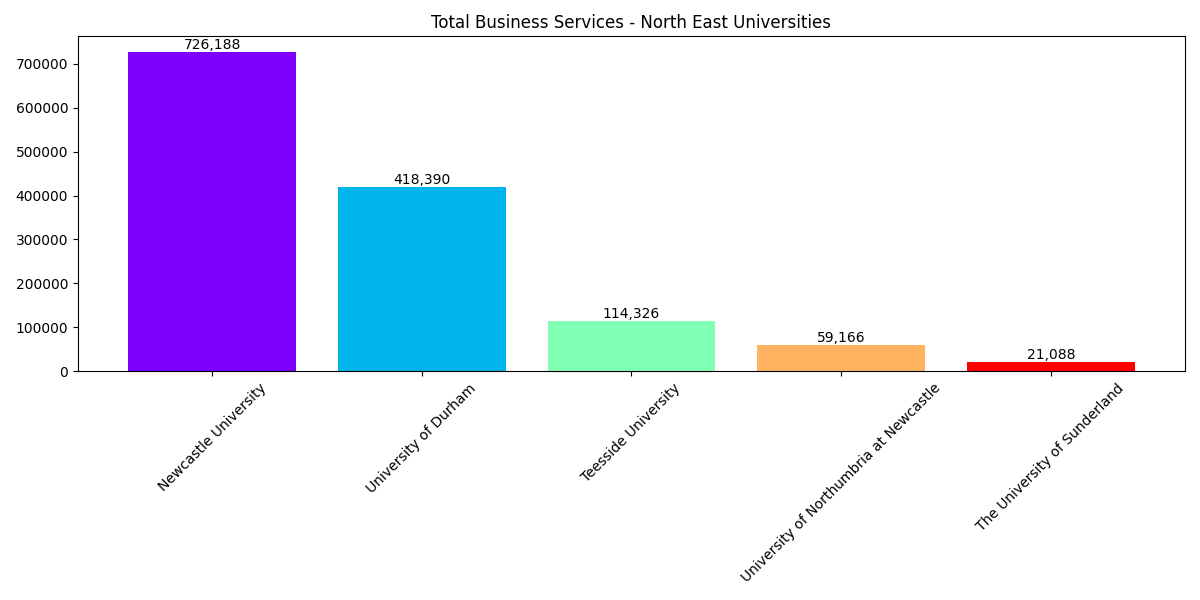
\includegraphics[width=0.8\textwidth]{Fig/figure10.services_ne_comparison.png}
\caption{Business Services - North East Universities Comparison}
\label{fig:services-ne-comparison}
\end{figure}

The business services portfolio shows a well-balanced distribution between contract research and consultancy, with a strong focus on non-commercial organizations. The above-average performance in this area suggests effective engagement with external partners and successful commercialization of university expertise. Table~\ref{tab:business-services-analysis} presents the detailed breakdown of service types, client organizations, and performance metrics, while Figure~\ref{fig:services-ne-comparison} shows Durham's competitive position within the North East region.

\subsubsection{CPD and Continuing Education}

Durham University delivered 98,190 learner days through CPD and continuing education courses, generating \textsterling 8,357 in revenue. The revenue breakdown shows that non-commercial organisations contributed the largest share (\textsterling 4,426), followed by individual learners (\textsterling 2,354), other commercial businesses (\textsterling 1,521), and SMEs (\textsterling 56), reflecting wide outreach but limited financial yield.

The activity involved 98,190 learner days and generated \textsterling 8,357 in revenue, highlighting a substantial investment of academic time and institutional effort in delivering CPD and continuing education, even though the income per learner day remained relatively low at \textsterling 0.085. Durham ranked fifth in the North East for CPD income, trailing behind Northumbria (\textsterling 74,062), Teesside (\textsterling 71,538), Newcastle (\textsterling 24,849), and Sunderland (\textsterling 14,229). Nationally, Durham ranked 123rd out of 228 institutions and was \textsterling 21,669 below the national average, suggesting an opportunity for growth in monetizing its CPD offerings.

Table~\ref{tab:cpd-analysis} illustrates the distribution of CPD activities across different categories and organizational types, providing insights into Durham's continuing education portfolio structure. While the CPD activities show significant time investment in terms of learner days, the financial returns are relatively low compared to other regional universities. This suggests potential for optimization in CPD delivery and pricing strategies to better align with market expectations.
\vspace{0.3cm}
\begin{table}[h]
\centering
\caption{CPD and Continuing Education Analysis - Durham University}
\vspace{0.1cm}
\resizebox{0.7\textwidth}{!}{%
\begin{tabular}{|l|r|r|r|}
\hline \textbf{CPD Category} & \textbf{Revenue (\textsterling)} & \textbf{Percentage} & \textbf{Notes} \\
\hline CE and CPD for individuals & 2,354 & 28.2\% & Individual learners \\
\hline Non-commercial organisations & 4,426 & 53.0\% & Primary client base \\
\hline Other (non-SME) commercial businesses & 1,521 & 18.2\% & Large commercial clients \\
\hline SMEs & 56 & 0.7\% & Small business clients \\
\hline \textbf{Total CPD Revenue} & \textbf{8,357} & \textbf{100.0\%} & \textbf{Revenue per day: \textsterling 0.085} \\
\hline \multicolumn{3}{|l|}{\textbf{Total Learner Days: 98,190}} & \textbf{National Rank: 123/228} \\
\hline \multicolumn{3}{|l|}{\textbf{National Average: \textsterling 30,026}} & \textbf{Difference: -\textsterling 21,669} \\
\hline
\end{tabular}
}
\label{tab:cpd-analysis}
\end{table}

\begin{figure}[h]
\centering
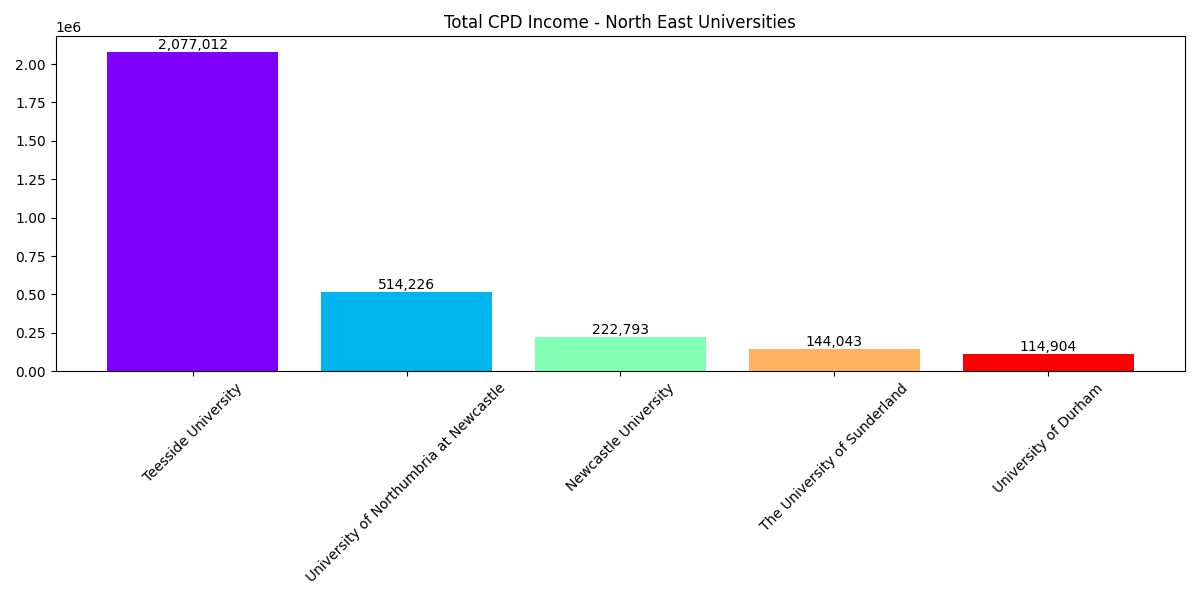
\includegraphics[width=0.8\textwidth]{Fig/figure13.cpd_ne_comparison.png}
\caption{CPD - North East Universities Comparison}
\label{fig:cpd-ne-comparison}
\end{figure}

The CPD analysis reveals Durham's strong engagement in continuing education delivery, with 98,190 learner days recorded, though financial returns remain below regional peers.

\subsubsection{Regeneration and Development}

Durham University reported a total of \textsterling 13,272 in regeneration and development income, with capital income accounting for \textsterling 13,026 (98.1\%). Additional sources included ERDF (\textsterling 4,171), UK government funds (\textsterling 3,989), the UK Shared Prosperity Fund (\textsterling 1,119), other regeneration grants (\textsterling 945), and miscellaneous sources (\textsterling 3,048), demonstrating a varied funding profile.

In the North East region, Durham ranked third in regeneration income, following Sunderland (\textsterling 33,972) and Teesside (\textsterling 23,224), but ahead of Newcastle (\textsterling 11,970) and Northumbria (\textsterling 3,828). On the national scale, Durham placed 52nd out of 228 universities and performed \textsterling 2,407 above the national average, indicating competitive positioning despite modest overall amounts.

Figures~\ref{fig:regeneration-programme}, \ref{fig:regeneration-time-trend}, and \ref{fig:regeneration-ne-comparison} provide detailed visualizations of Durham's regeneration programme distribution, temporal trends, and regional positioning. The regeneration and development activities, though smaller in scale compared to other income streams, perform above the national average and maintain a competitive position in the region. The diverse funding sources indicate successful engagement with various regeneration initiatives.

\begin{figure}[h]
\centering
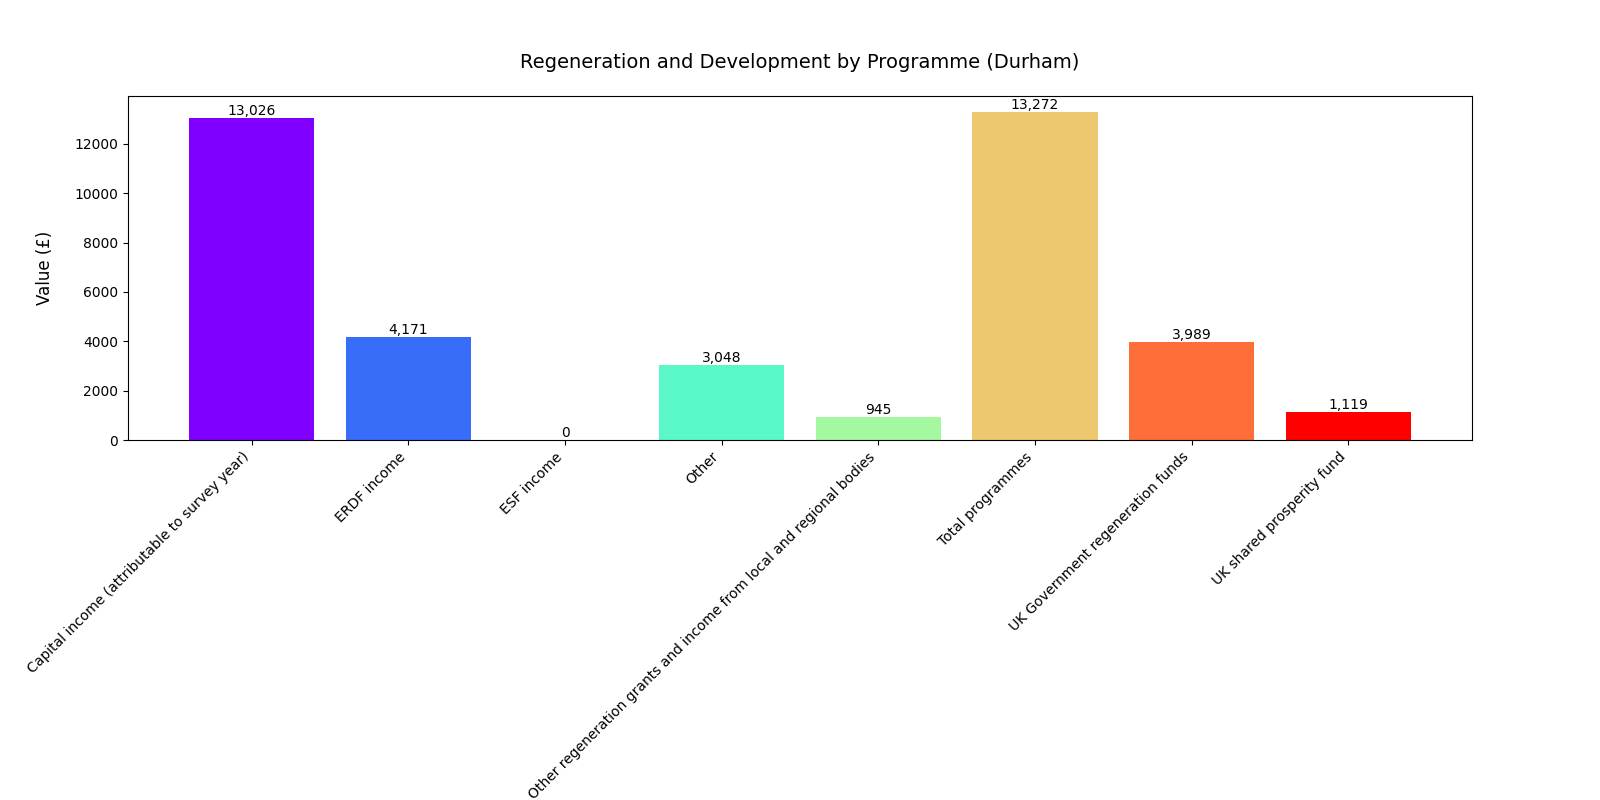
\includegraphics[width=0.9\textwidth]{Fig/figure14.regeneration_programme.png}
\caption{Regeneration Programme Distribution}
\label{fig:regeneration-programme}
\end{figure}

\begin{figure}[h]
\centering
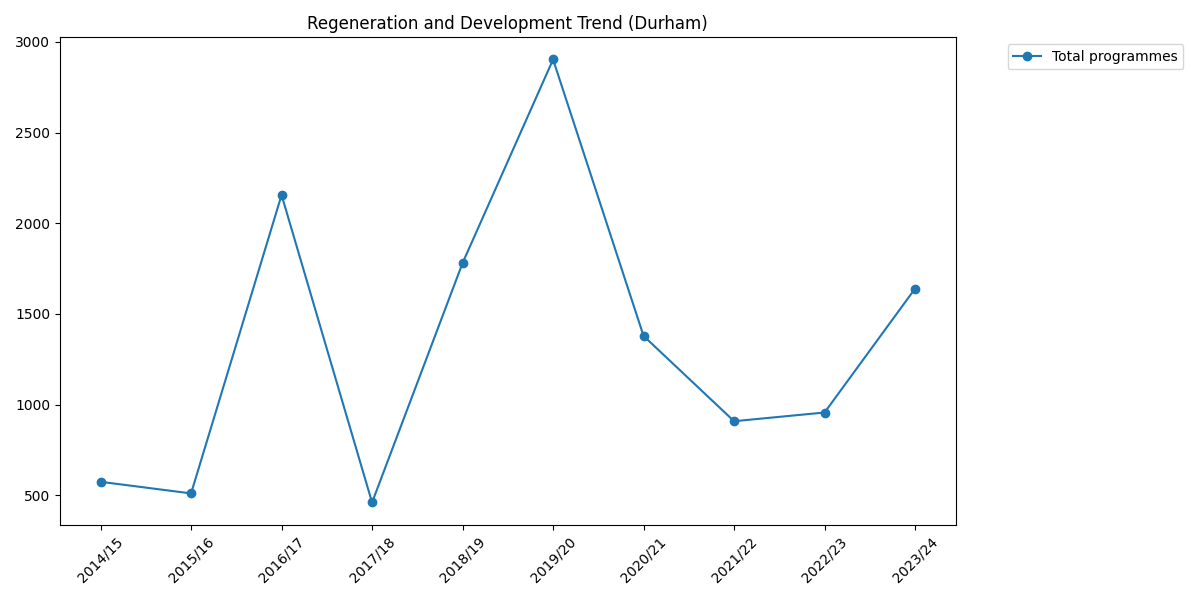
\includegraphics[width=0.7\textwidth]{Fig/figure15.regeneration_time_trend.png}
\caption{Regeneration and Development Income Trends (2019-2023)}
\label{fig:regeneration-time-trend}
\end{figure}

\begin{figure}[h]
\centering
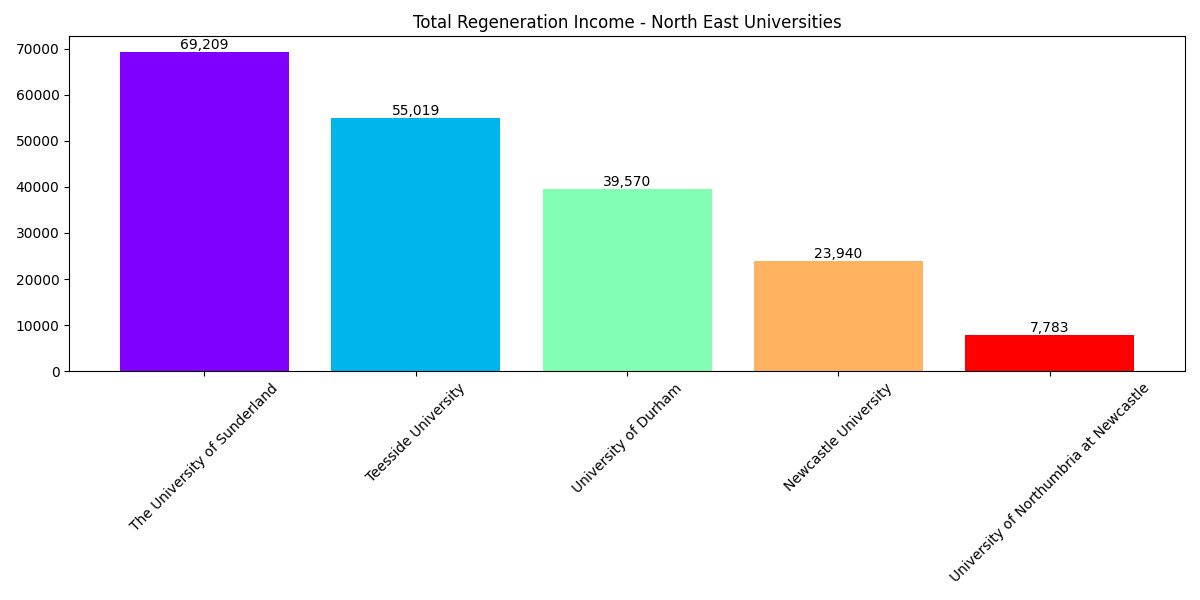
\includegraphics[width=0.8\textwidth]{Fig/figure16.regeneration_ne_comparison.png}
\caption{Regeneration - North East Universities Comparison}
\label{fig:regeneration-ne-comparison}
\end{figure}

The regeneration analysis demonstrates Durham's effective engagement with various funding sources and regional development initiatives.

\subsubsection{Overall Performance}

With a total income of \textsterling 396,114 from all categories, Durham ranked second overall in the North East, behind Newcastle University (\textsterling 1,489,132). It outperformed Northumbria (\textsterling 239,042), Teesside (\textsterling 216,785), and Sunderland (\textsterling 60,776), reaffirming its position as a top-tier institution in the region.

The breakdown of income shows that research income is Durham's largest revenue source at 54.7\% (\textsterling 216,850), followed by business services (39.8\% or \textsterling 157,635), regeneration and development (3.4\% or \textsterling 13,272), and CPD and continuing education (2.1\% or \textsterling 8,357). This indicates a diverse yet research-focused funding profile.

Figure~\ref{fig:overall-performance} provides a comprehensive overview of Durham's total income composition and regional ranking. Durham University's income profile reflects a well-diversified portfolio with business services as the primary driver. The strong performance in business services and research, combined with above-average regeneration activities, positions the university competitively in the North East region. However, the relatively lower performance in CPD activities suggests an area for potential improvement and strategic focus.

\begin{figure}[h]
\centering
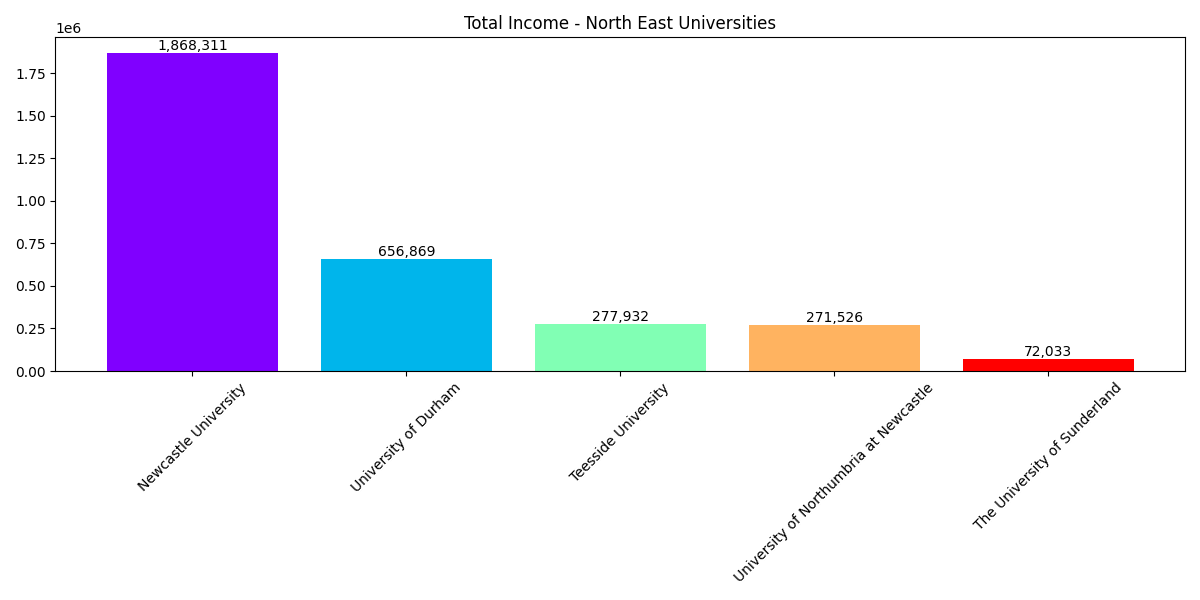
\includegraphics[width=0.8\textwidth]{Fig/figure17._overall_performance.png}
\caption{Overall performance}
\label{fig:overall-performance}
\end{figure}

The overall performance analysis confirms Durham's strong regional positioning and diversified income structure. The income analysis reveals Durham University's strong performance in research income, ranking 33rd nationally with a total of \textsterling 216,850. The university demonstrates a well-diversified income portfolio, with significant contributions from research and business services. While research income shows some volatility, business services income (\textsterling 157,635) provides a stable revenue stream, and CPD income, despite high learner engagement (98,190 learner days), generates relatively low revenue (\textsterling 8,357). The university's total income of \textsterling 396,114 positions it second in the North East region, indicating a solid financial foundation with research as the primary driver.

\subsection{Intellectual Property Analysis}
\label{sec:ip-analysis}

\subsubsection{IP Disclosures and Patents}

\begin{itemize}
    \item \textbf{Disclosure Distribution:} Durham University reported a total of 3,458 IP disclosures, maintaining a cumulative patent portfolio of 2,019 patents. In the most recent year, 124 new patent applications were filed, and 80 patents were granted, including 631 cumulative overseas patents. These figures indicate steady and active participation in intellectual property development and protection.
    
    \item \textbf{National Position:} Durham ranked 28th out of 228 universities nationwide in total IP disclosures, surpassing the national average of 2,076 by 1,382 disclosures. This reflects Durham's strong commitment to innovation and technology transfer compared to peer institutions.
    
    \item \textbf{Regional Comparison:} Regionally, Durham held the second-highest position in the North East for IP disclosures, behind Newcastle University (5,600), and significantly ahead of other institutions in the region.
\end{itemize}

Durham University demonstrates strong IP generation capabilities, supported by a substantial patent portfolio and active patenting activity. The above-average performance in disclosures indicates effective research commercialization and a productive innovation pipeline. Figure~\ref{fig:ip-disclosure-type}, and Figure~\ref{fig:ip-ne-comparison} illustrate Durham's IP disclosure patterns, temporal trends, and regional positioning in intellectual property development.



\begin{figure}[h]
\centering
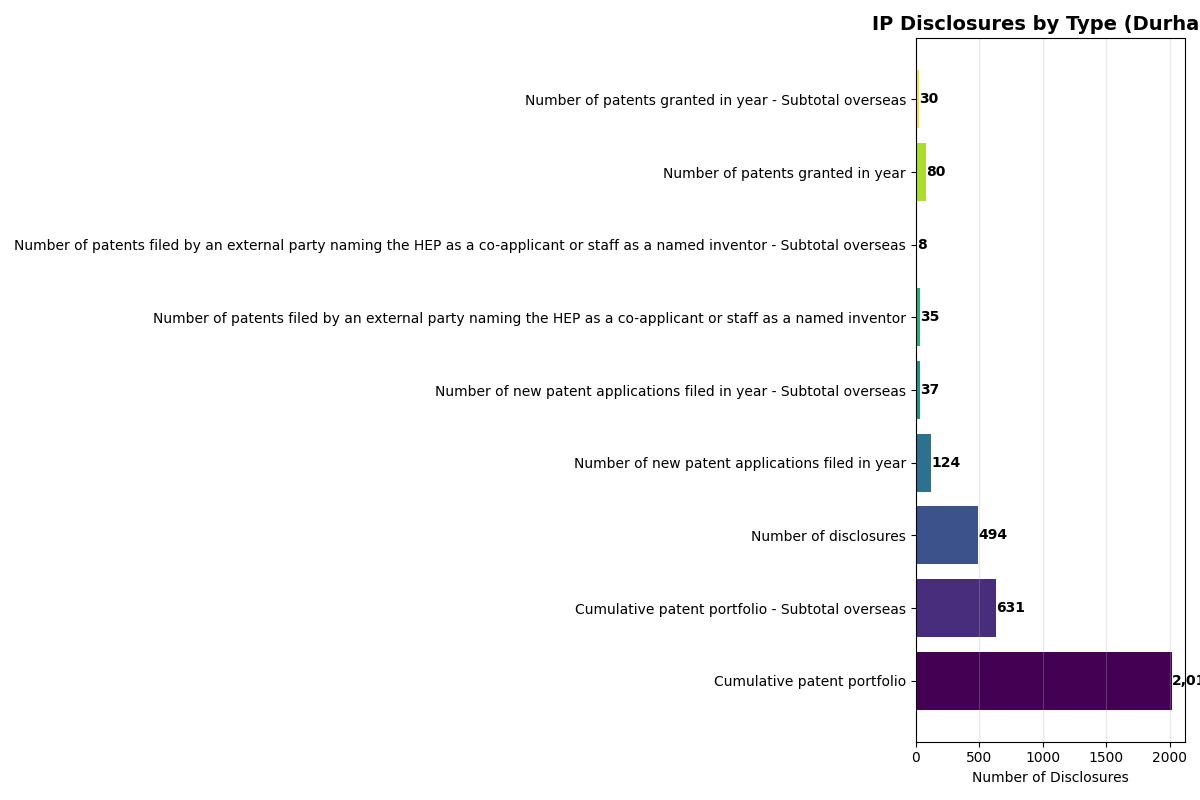
\includegraphics[width=0.8\textwidth]{Fig/figure18.ip_disclosure_type.png}
\caption{IP Disclosure Types Comparison}
\label{fig:ip-disclosure-type}
\end{figure}

% \begin{figure}[h]
% \centering
% 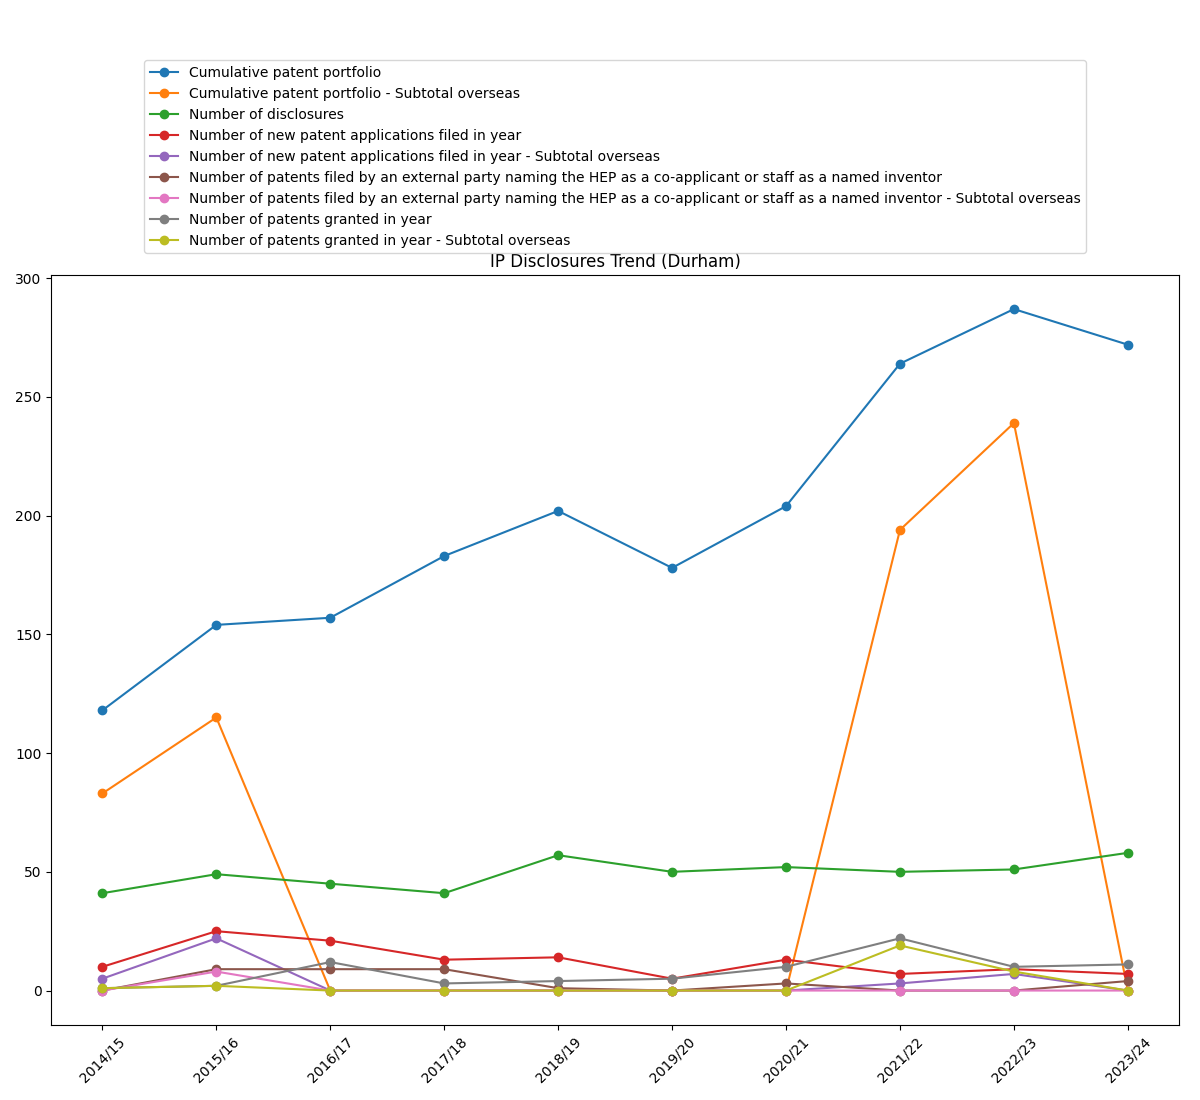
\includegraphics[width=0.8\textwidth]{Fig/figure19.ip_disclosure_trend.png}
% \caption{IP Disclosure Trend Analysis}
% \label{fig:ip-disclosure-trend}
% \end{figure}

\begin{figure}[h]
\centering
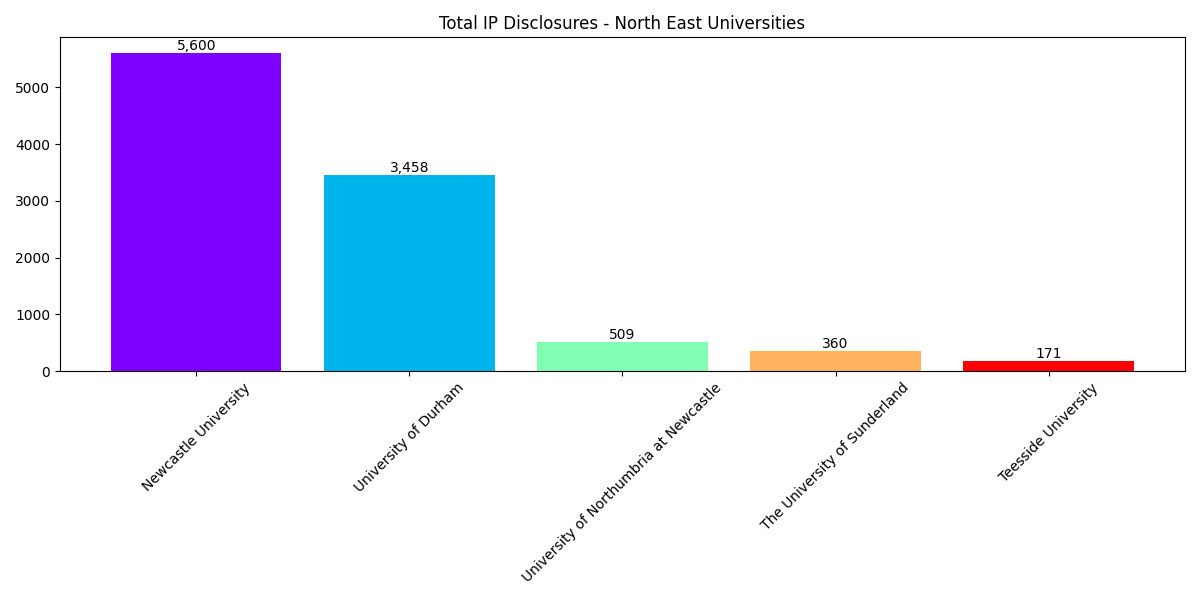
\includegraphics[width=0.8\textwidth]{Fig/figure20.ip_ne_comparison.png}
\caption{IP Disclosures - North East Universities Comparison}
\label{fig:ip-ne-comparison}
\end{figure}

\subsubsection{License Analysis}

Durham reported a total of 808 active licenses, comprising 691 non-software and 117 software licenses. However, only 30 of these licenses were income-generating, highlighting a gap between licensing activity and financial returns.

Among the license recipients, SMEs accounted for the largest share (412 licenses), followed by other commercial businesses (251) and non-commercial organizations (145). This distribution suggests a strong alignment with small business and applied-sector engagement. Durham ranked second in the North East for license volume, trailing Newcastle University (1,514 licenses), and held the 35th position nationally among 228 universities.

Table~\ref{tab:license-analysis} provides detailed breakdowns of license types, client organizations, and regional comparisons. Although Durham has built a sizable licensing portfolio, the relatively low number of income-generating licenses points to untapped potential in IP commercialization. The high proportion of licenses with SMEs suggests effective engagement with smaller enterprises, but there remains room to strengthen financial outcomes from licensing activity.
\vspace{0.2cm}
\begin{table}[h]
\centering
\caption{IP License Analysis - Durham University}
\vspace{0.1cm}
\resizebox{0.9\textwidth}{!}{%
\begin{tabular}{|l|l|r|r|r|}
\hline \textbf{License Type} & \textbf{Organization Type} & \textbf{License Count} & \textbf{Income Generating} & \textbf{Income Generation Rate} \\
\hline \multirow{3}{*}{Non-software} & Non-commercial organisations & 129 & 5 & 3.9\% \\
\cline{2-5}
& Other (non-SME) commercial & 203 & 8 & 3.9\% \\
\cline{2-5}
& SMEs & 359 & 13 & 3.6\% \\
\hline \multirow{3}{*}{Software only} & Non-commercial organisations & 16 & 1 & 6.2\% \\
\cline{2-5}
& Other (non-SME) commercial & 48 & 2 & 4.2\% \\
\cline{2-5}
& SMEs & 53 & 1 & 1.9\% \\
\hline \multicolumn{2}{|l|}{\textbf{Total Licenses}} & \textbf{808} & \textbf{30} & \textbf{3.7\%} \\
\hline \multicolumn{2}{|l|}{\textbf{National Performance}} & \textbf{Rank: 35/228} & \textbf{National Average: 2,258} & \textbf{Difference: -1,450} \\
\hline
\end{tabular}
}
\label{tab:license-analysis}
\end{table}

\begin{figure}[h]
\centering
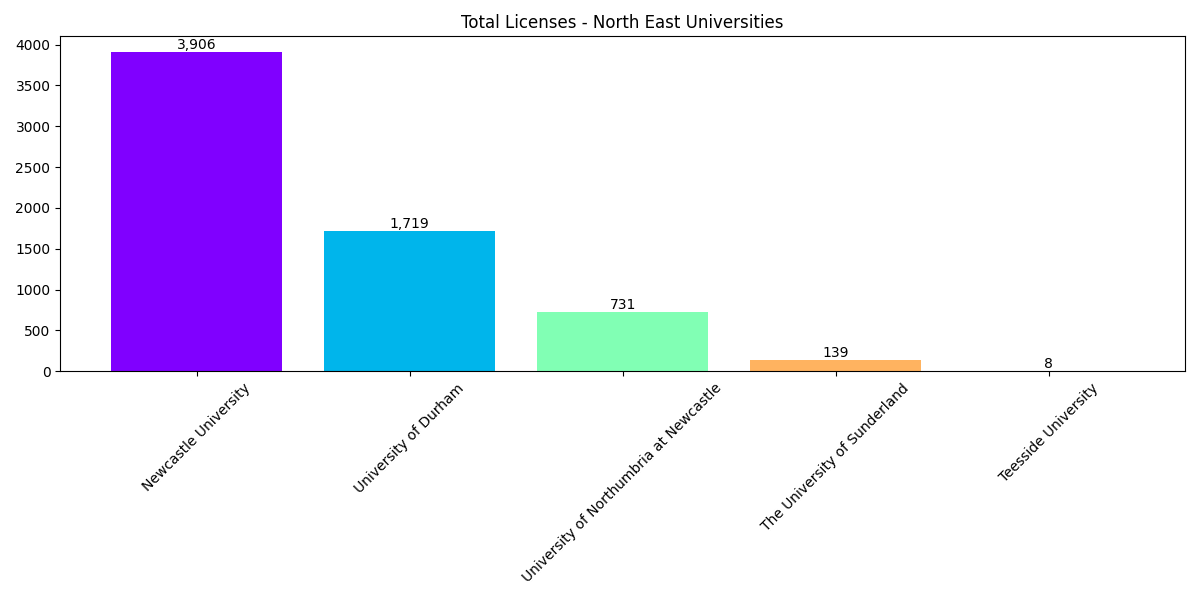
\includegraphics[width=0.8\textwidth]{Fig/figure23.license_ne_comparison.png}
\caption{IP Licenses - North East Universities Comparison}
\label{fig:license-ne-comparison}
\end{figure}

The license analysis reveals Durham's extensive portfolio but highlights opportunities for improved commercialization outcomes.

\subsubsection{IP Income}

Durham generated a total of \textsterling 6,687 in IP-related income, with the majority (\textsterling 5,961 or 89.1\%) coming from the sale of shares in spin-out companies. Traditional IP licensing activities contributed \textsterling 726 (10.9\%), including \textsterling 517 from non-software licenses, \textsterling 49 from software licenses, and \textsterling 160 from other IP sources. This distribution reflects Durham's strong performance in spin-out company development but limited direct licensing revenue.

Income by client type for licensing activities showed that SMEs contributed \textsterling 458, followed by other commercial businesses (\textsterling 163) and non-commercial organizations (\textsterling 105), indicating generally low monetization across all sectors. In the North East, Durham ranked second in total IP income, behind Newcastle University (\textsterling 36,868), and held the 34th position nationally out of 228 universities.



Durham's IP income performance is well below the national average, underscoring the need for improved strategies to monetize its intellectual property. Despite an active licensing environment, the low revenue figures highlight the importance of enhancing commercialization effectiveness.
\vspace{0.2cm}
\begin{table}[h]
\centering
\caption{IP Income Analysis - Durham University}
\resizebox{0.8\textwidth}{!}{%
\begin{tabular}{|l|l|r|r|}
\hline \textbf{Income Source} & \textbf{Organization Type} & \textbf{Income (\textsterling)} & \textbf{Percentage} \\
\hline \multirow{3}{*}{Non-software licenses} & Non-commercial organisations & 20 & 0.3\% \\
\cline{2-4}
& Other (non-SME) commercial & 108 & 1.6\% \\
\cline{2-4}
& SMEs & 389 & 5.8\% \\
\hline \multirow{3}{*}{Software licenses} & Non-commercial organisations & 17 & 0.3\% \\
\cline{2-4}
& Other (non-SME) commercial & 27 & 0.4\% \\
\cline{2-4}
& SMEs & 5 & 0.1\% \\
\hline \multirow{3}{*}{Other IP income} & Non-commercial organisations & 68 & 1.0\% \\
\cline{2-4}
& Other (non-SME) commercial & 28 & 0.4\% \\
\cline{2-4}
& SMEs & 64 & 1.0\% \\
\hline \multirow{2}{*}{Sale of shares in spin-outs} & All types & 5,961 & 89.1\% \\
\cline{2-4}
& \multicolumn{2}{|l|}{\textbf{Subtotal IP Income}} & \textbf{726 (10.9\%)} \\
\hline \multicolumn{2}{|l|}{\textbf{Total IP Income}} & \textbf{6,687} & \textbf{100.0\%} \\
\hline \multicolumn{2}{|l|}{\textbf{National Performance}} & \textbf{Rank: 34/228} & \textbf{National Average: \textsterling 10,803} \\
\hline
\end{tabular}
}
\label{tab:ip-income-analysis}
\end{table}

\begin{figure}[h]
\centering
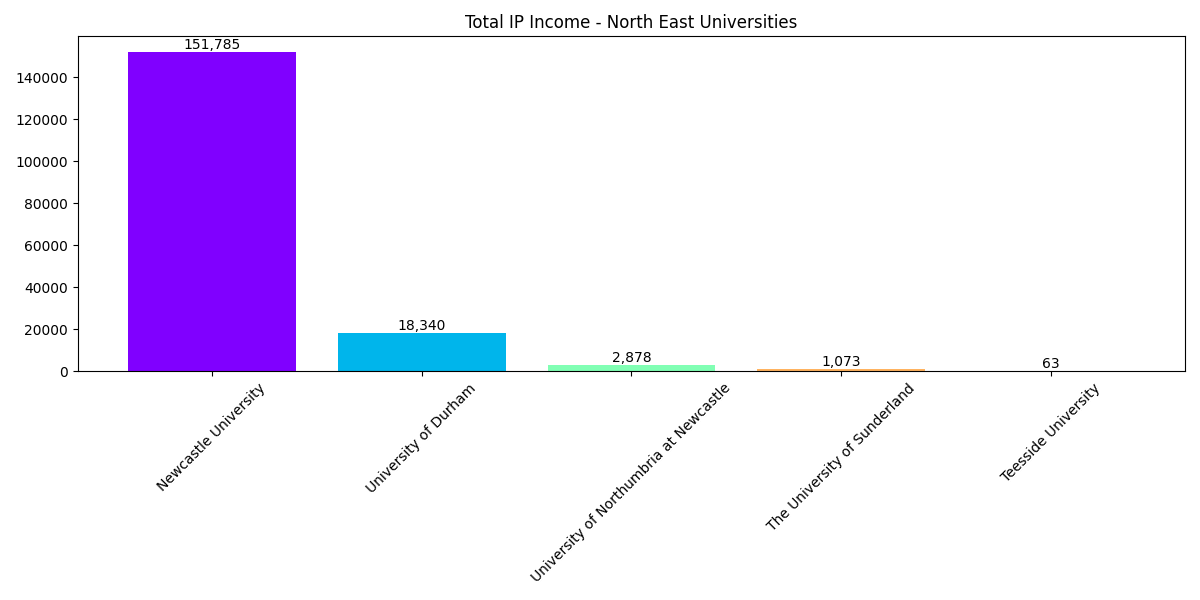
\includegraphics[width=0.8\textwidth]{Fig/figure26.ip_income_ne_comparison.png}
\caption{IP Income - North East Universities Comparison}
\label{fig:ip-income-ne-comparison}
\end{figure}

Durham's IP income performance is well below the national average, underscoring the need for improved strategies to monetize its intellectual property. Despite an active licensing environment, the low revenue figures highlight the importance of enhancing commercialization effectiveness.

\subsubsection{Spin-off Companies}

\begin{itemize}
    \item \textbf{Company Metrics:} Durham University supported 642 active spin-off firms, which together employed 5,455 full-time equivalent (FTE) staff and generated a turnover of \textsterling 542.35 million. The firms attracted \textsterling 117.66 million in external investment and included 185 newly created companies, indicating robust entrepreneurial output.
    
    \item \textbf{Company Types:} Of these companies, spin-outs with university ownership generated \textsterling 396.09 million in turnover, other spin-outs contributed \textsterling 262.33 million, while student start-ups accounted for \textsterling 8.12 million. The ecosystem also included 15 staff start-ups and 4 social enterprises, demonstrating a diverse entrepreneurial landscape.
    
    \item \textbf{Regional Position:} Durham ranked third in the North East in spin-off activity, following Newcastle University (\textsterling 1.59 billion) and Northumbria (\textsterling 1.03 billion), and was 25th nationally out of 228 universities.
\end{itemize}



Durham shows strong performance in spin-off activity, with significant economic impact in terms of employment, revenue, and external investment. The university's support for both university-owned and student-led ventures highlights the success of its entrepreneurship and technology transfer frameworks.

\begin{figure}[h]
    \centering
    \begin{subfigure}[b]{0.425\textwidth}
        \centering
        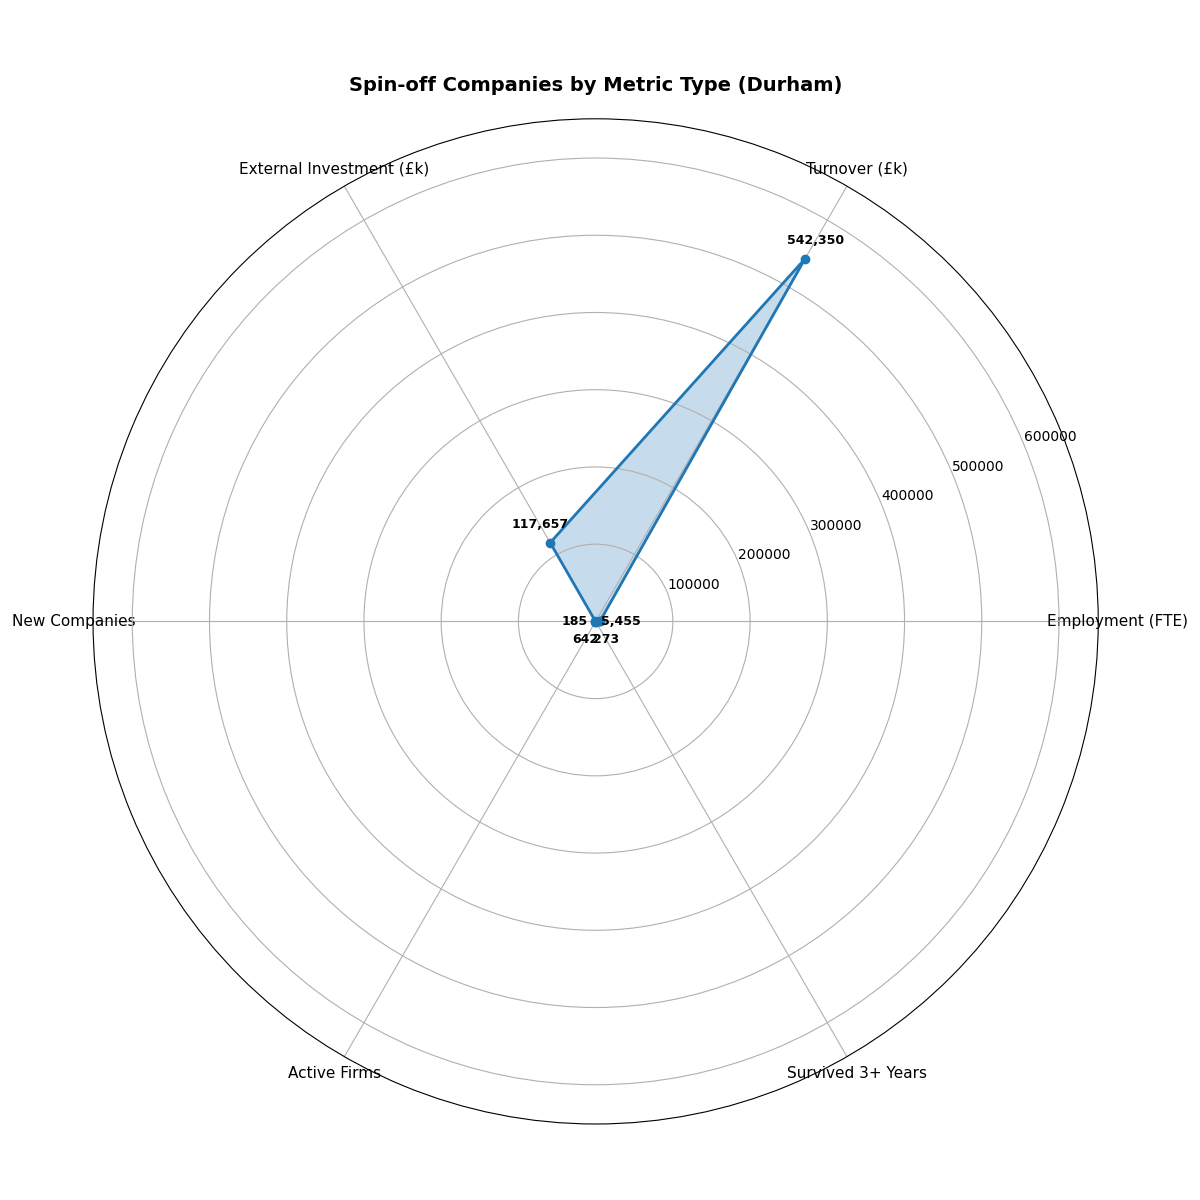
\includegraphics[width=\linewidth]{Fig/figure27.spin_metric_type.png}
        \caption{Spin-off Company Metrics - Radar Chart}
        \label{fig:spin-metric-type}
    \end{subfigure}
    \hspace{0.05\textwidth} 
    \begin{subfigure}[b]{0.5\textwidth}
        \centering
        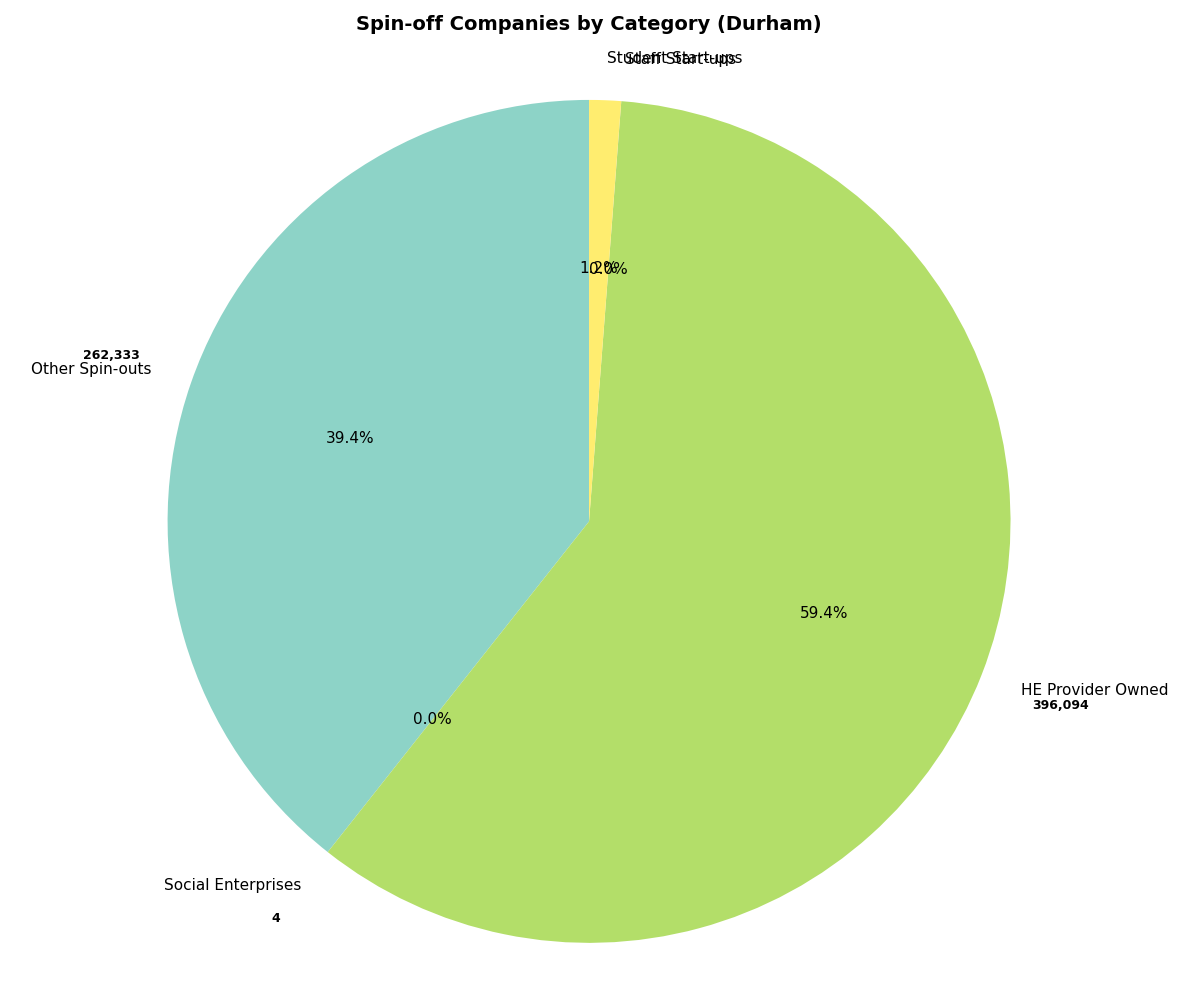
\includegraphics[width=\linewidth]{Fig/figure28.spin_category.png}
        \caption{Spin-off Company Categories - Pie Chart}
        \label{fig:spin-category}
    \end{subfigure}
    \vspace{0.65cm}
    \caption{Spin-off Company Analysis}
    \label{fig:spin-analysis}
\end{figure}

\begin{figure}[h]
\centering
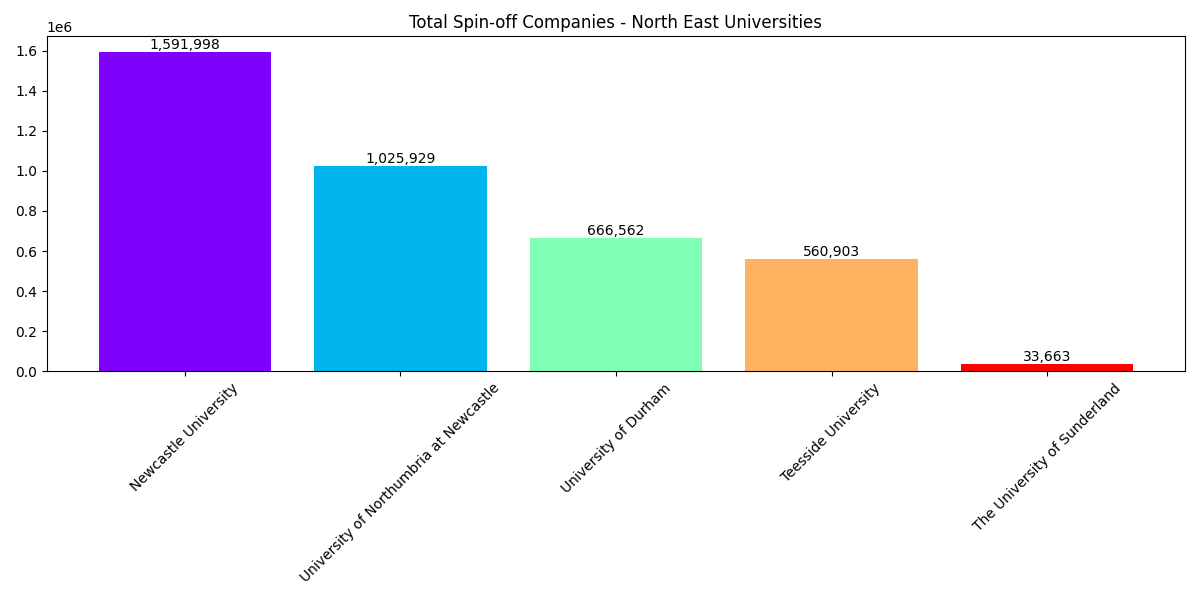
\includegraphics[width=0.8\textwidth]{Fig/figure29.spin_ne_comparison.png}
\caption{Spin-off Companies - North East Universities Comparison}
\label{fig:spin-ne-comparison}
\end{figure}

Durham shows strong performance in spin-off activity, with significant economic impact in terms of employment, revenue, and external investment. The university's support for both university-owned and student-led ventures highlights the success of its entrepreneurship and technology transfer frameworks.

\subsubsection{Overall IP Performance}

Durham University presents a well-developed IP ecosystem with notable strengths in disclosure volume and spin-off creation. However, the relatively low IP income and limited number of income-generating licenses suggest a need to enhance commercialization practices. As a leading IP generator in the North East, Durham is well-positioned to improve financial returns by better leveraging its innovations and expanding its impact through strategic industry engagement. The IP analysis highlights Durham University's strong performance in IP generation and management, ranking 31st nationally in IP disclosures and maintaining a consistent second position in the North East region. The analysis shows a balanced portfolio of IP activities, with particular strength in patent applications and technology disclosures. However, the IP income generation shows some volatility, suggesting opportunities for improvement in commercialization strategies. The university's spin-off company performance is above average, indicating effective translation of research into commercial ventures.

\subsection{Public Engagement Analysis}
\label{sec:public-engagement}

\subsubsection{Event Nature and Type Analysis}

Durham University hosted a total of 6,043,792 public engagement events, of which 72.1\% (4,356,662) were free and 27.9\% (1,687,130) were chargeable. This indicates a strong institutional commitment to accessibility and public service through freely available educational and cultural offerings.

The majority of events (68.8\%, or 4,160,059) were categorized as "Other," suggesting a broad and possibly innovative approach to engagement activities. More traditional formats also featured prominently, including exhibitions (19.3\%), museum education programs (5.5\%), public lectures (4.5\%), and performance arts (2.0\%). Durham ranks 31st out of 228 universities in total event count, trailing the national average of 29,012,765 by 22,968,973 events. Despite this, its focus on accessible programming and event diversity positions it well in terms of outreach quality and inclusivity.

The data reflect Durham University's extensive and diverse public engagement program. The predominance of free and non-traditional event formats signals a forward-thinking approach to community involvement that prioritizes accessibility and experimentation in outreach.

\begin{figure}[h]
\centering
\begin{subfigure}[b]{0.48\textwidth}
    \centering
    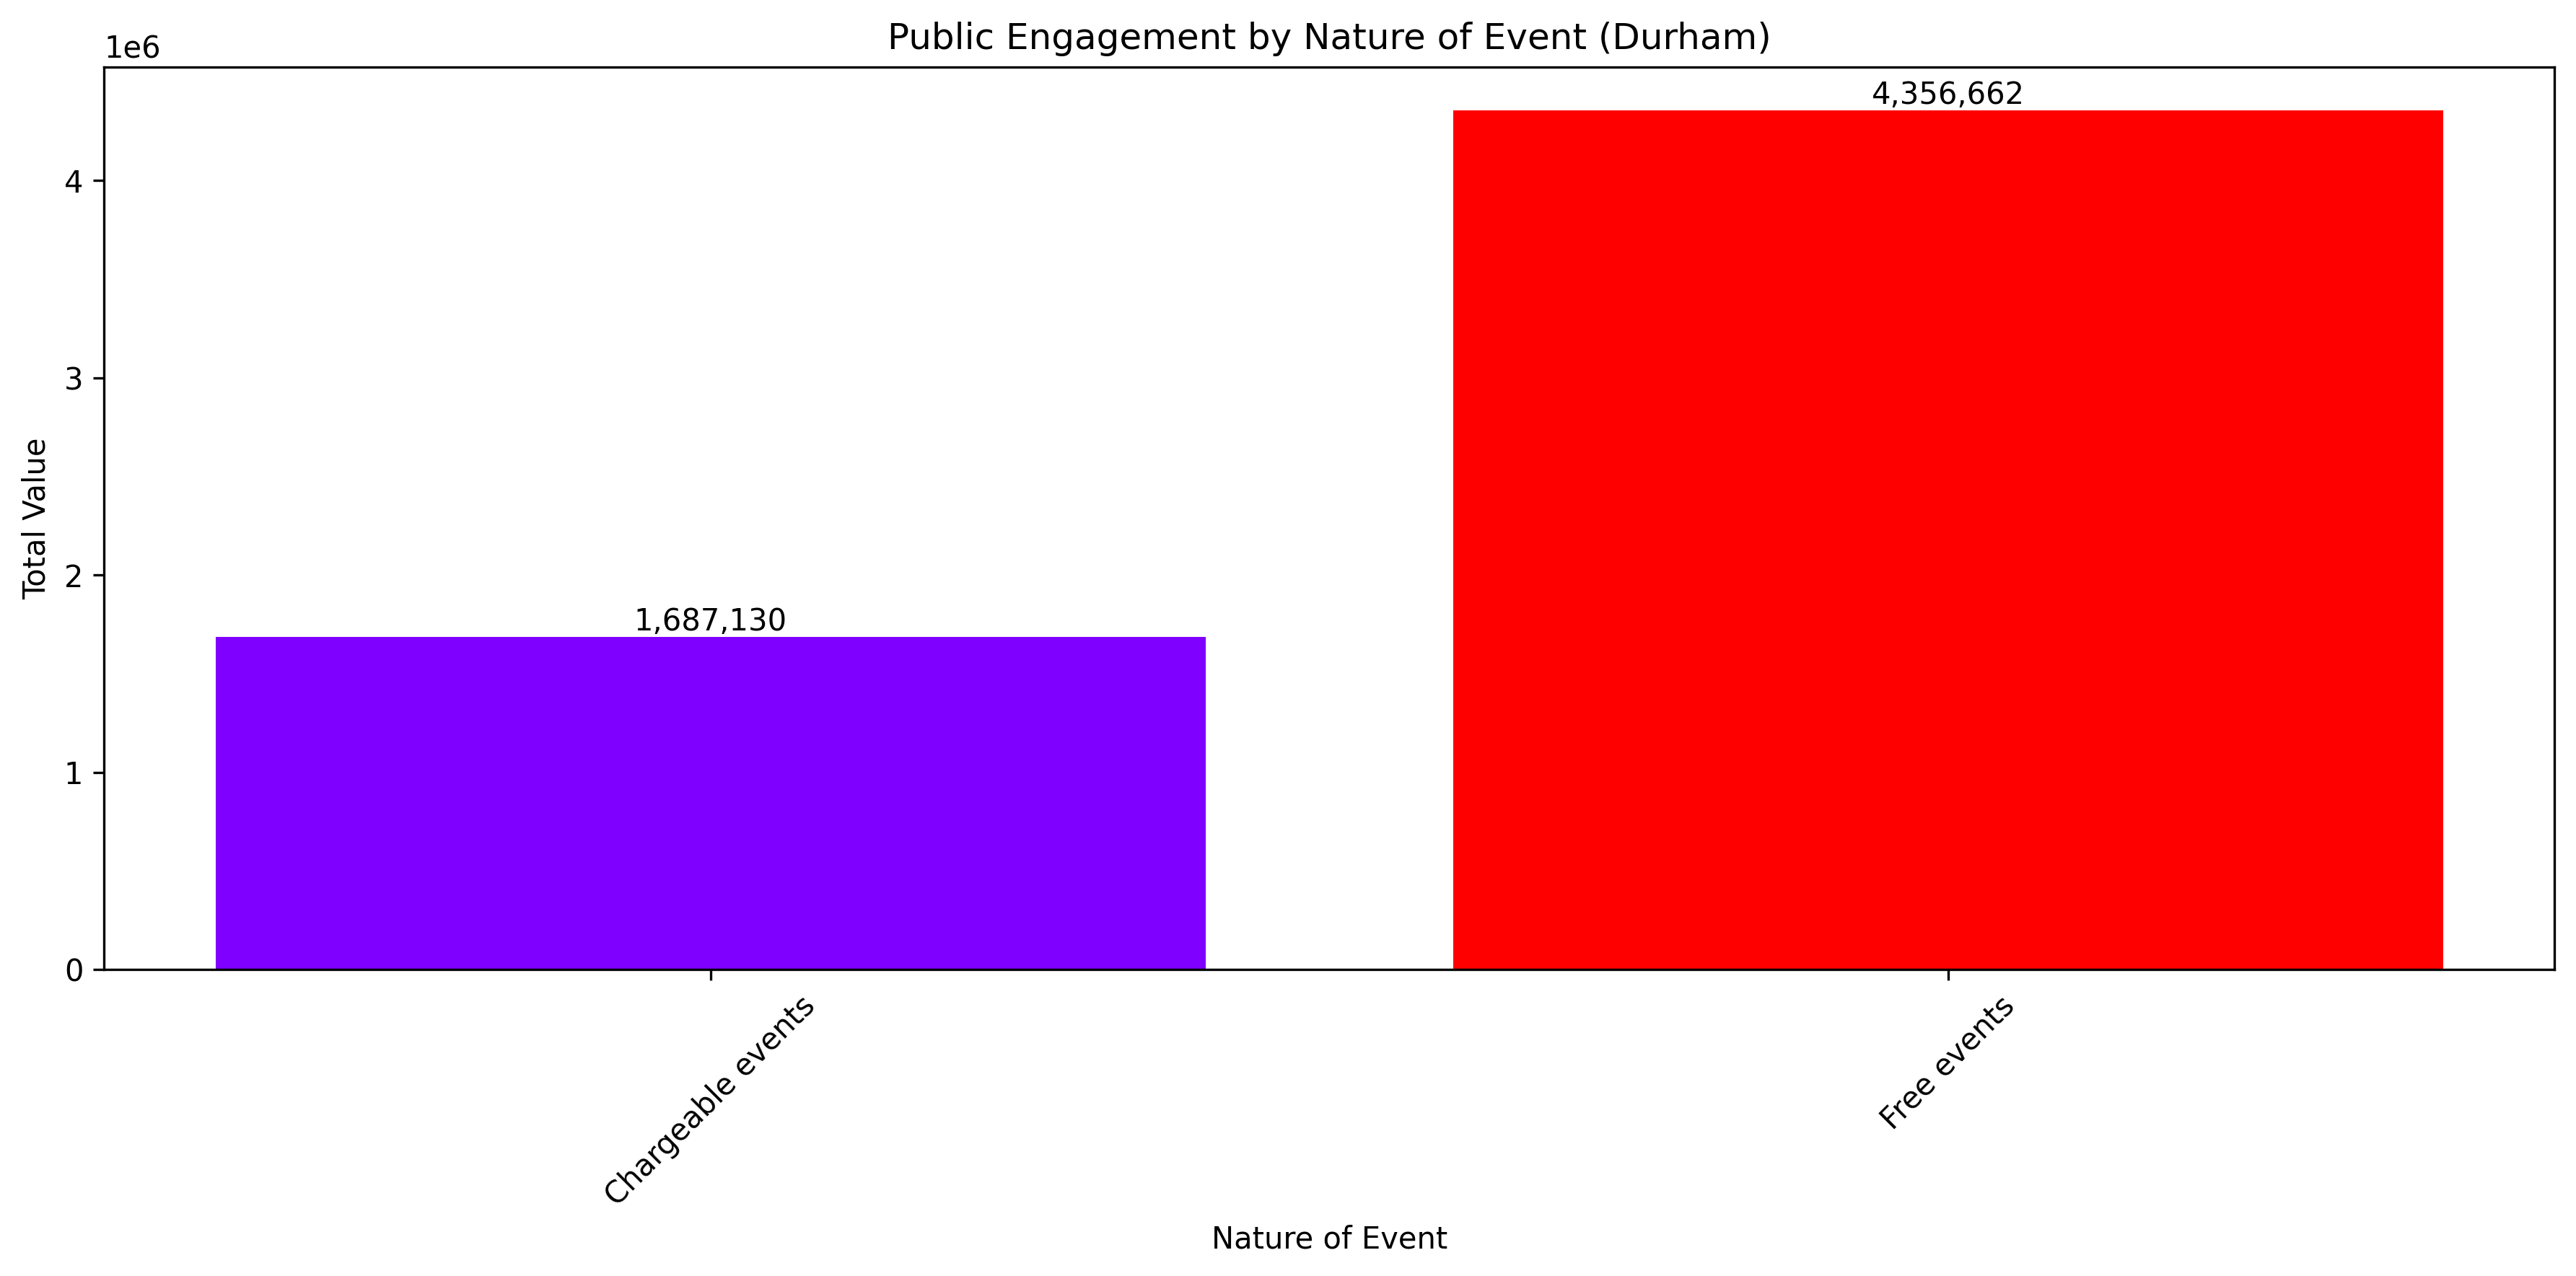
\includegraphics[width=\textwidth]{Fig/figure30.nature_of_event.png}
    \caption{Nature of event}
    \label{fig:nature-of-event}
\end{subfigure}
\hfill
\begin{subfigure}[b]{0.48\textwidth}
    \centering
    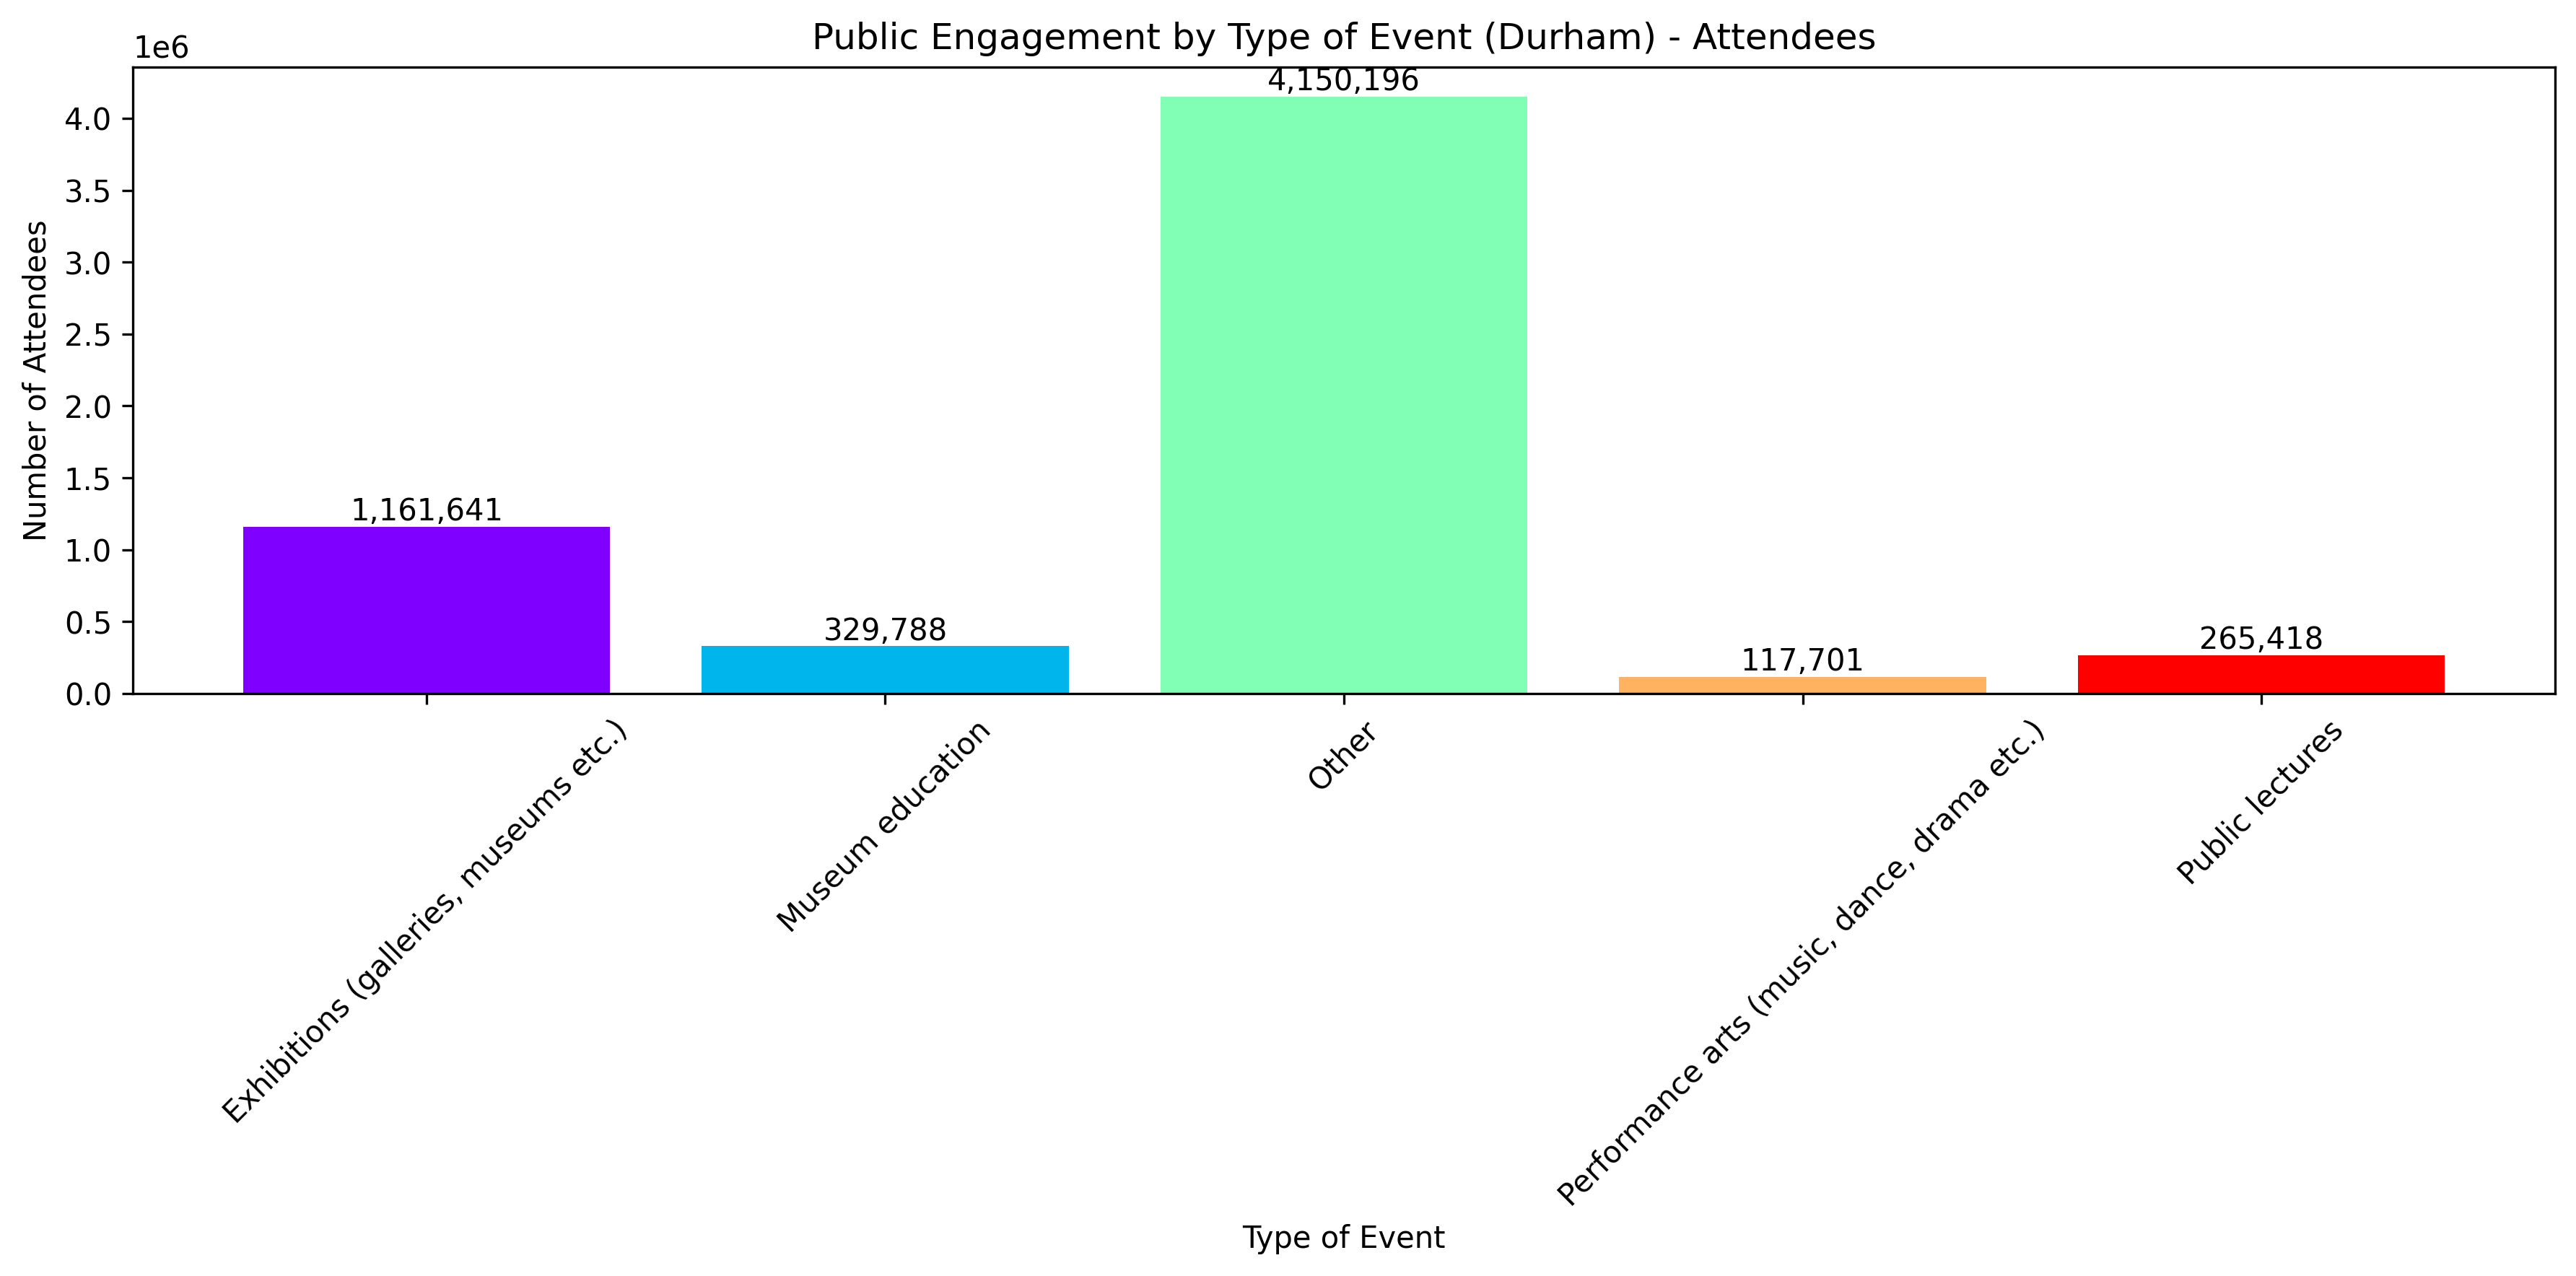
\includegraphics[width=\textwidth]{Fig/figure31.type_of_event.png}
    \caption{Type of event}
    \label{fig:type-of-event}
\end{subfigure}
\vspace{0.6cm}
\caption{Event Nature and Type Analysis}
\label{fig:event-analysis}
\end{figure}

The data reflect Durham University's extensive and diverse public engagement program. The predominance of free and non-traditional event formats signals a forward-thinking approach to community involvement that prioritizes accessibility and experimentation in outreach.

\subsubsection{Participation Analysis}

A total of 6,024,744 people participated in Durham's public engagement events. Most attendees (68.9\%) were involved in "Other" events, followed by exhibitions (19.3\%), museum education (5.5\%), public lectures (4.4\%), and performance arts (2.0\%). This aligns with the distribution of event types, further confirming the appeal of Durham's diverse engagement offerings.

Durham staff contributed 19,048 days to engagement efforts. Over half of this time (51.8\%) was devoted to "Other" events, while public lectures (23.2\%), museum education (12.4\%), exhibitions (10.3\%), and performance arts (2.3\%) also received significant support. This distribution suggests broad institutional participation across event formats.

Figure~\ref{fig:participation-analysis} presents a detailed breakdown of Durham's public engagement participation patterns, showing both attendee distribution by event type (left panel) and academic staff time allocation by event type (right panel). The left panel of Figure~\ref{fig:attendees-by-type} reveals that "Other" events attracted the largest number of participants (4,150,196), followed by exhibitions (1,161,641), museum education (329,788), public lectures (265,418), and performance arts (117,701). The right panel of Figure~\ref{fig:staff-time-by-type} demonstrates that staff time allocation closely mirrors attendee preferences, with "Other" events receiving the most staff support (9,863 days), followed by public lectures (4,425 days), museum education (2,367 days), exhibitions (1,961 days), and performance arts (432 days).

Durham's public engagement strategy benefits from significant audience reach and academic involvement. The strong alignment between event type popularity and staff time allocation reflects efficient and strategic resource use in community-facing activities.

\begin{figure}[h]
\centering
\begin{subfigure}[b]{0.48\textwidth}
    \centering
    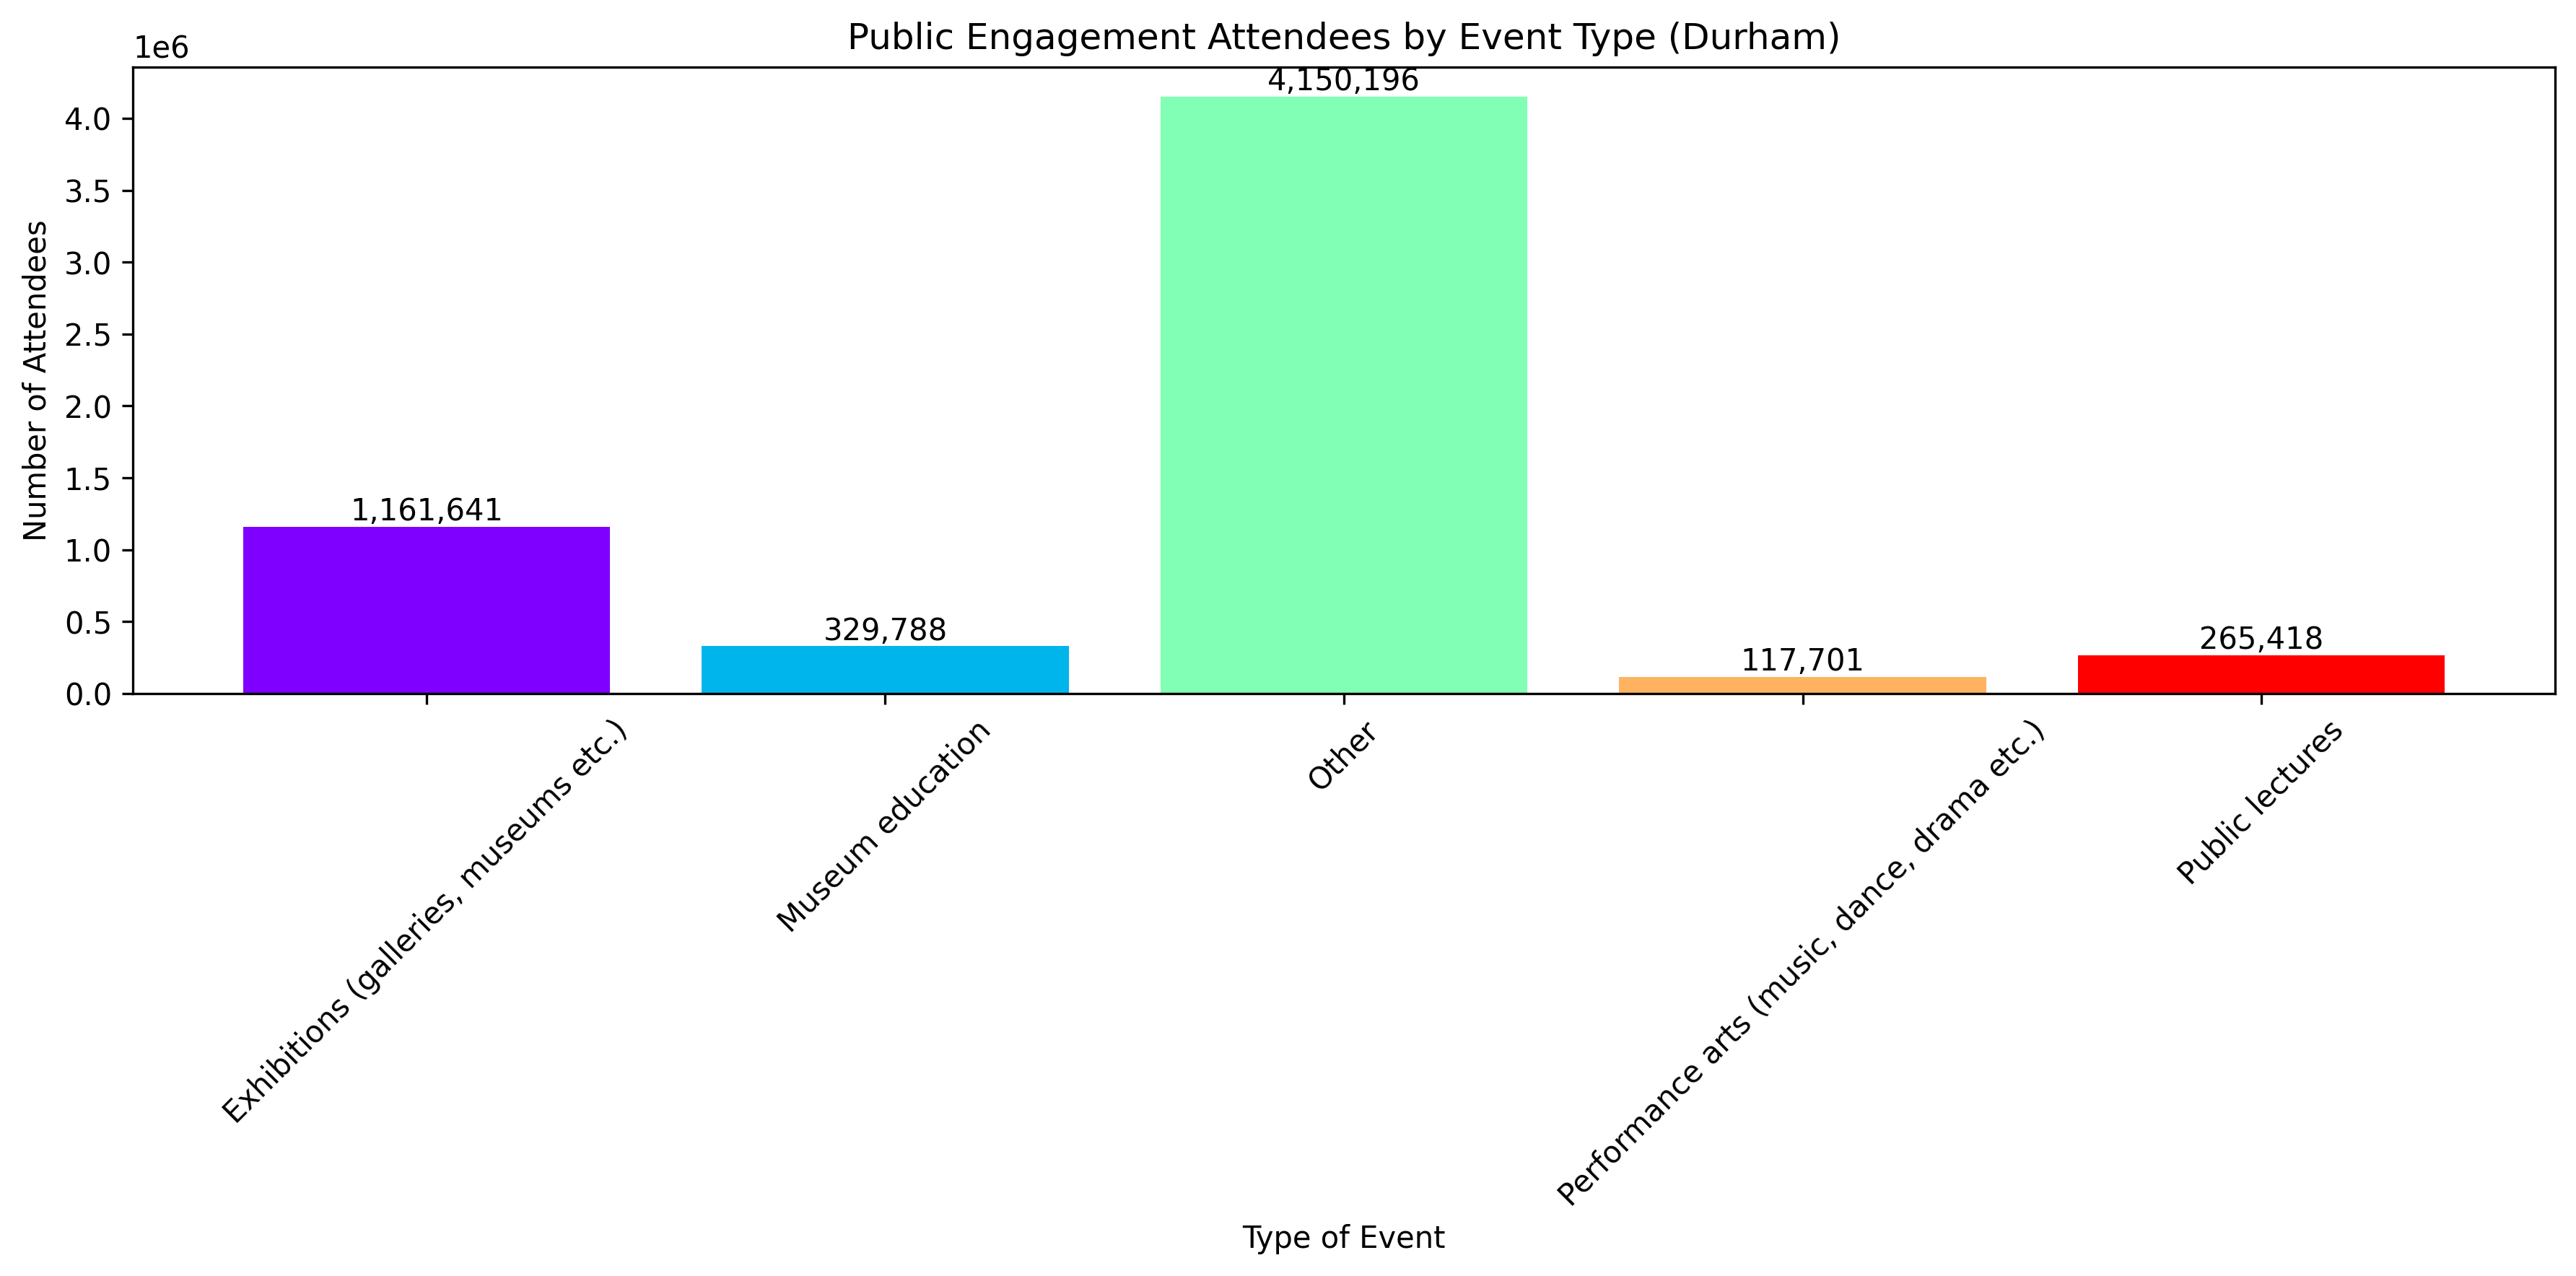
\includegraphics[width=\textwidth]{Fig/figure32.attendees_by_type.png}
    \caption{Type of attendee}
    \label{fig:attendees-by-type}
\end{subfigure}
\hfill
\begin{subfigure}[b]{0.48\textwidth}
    \centering
    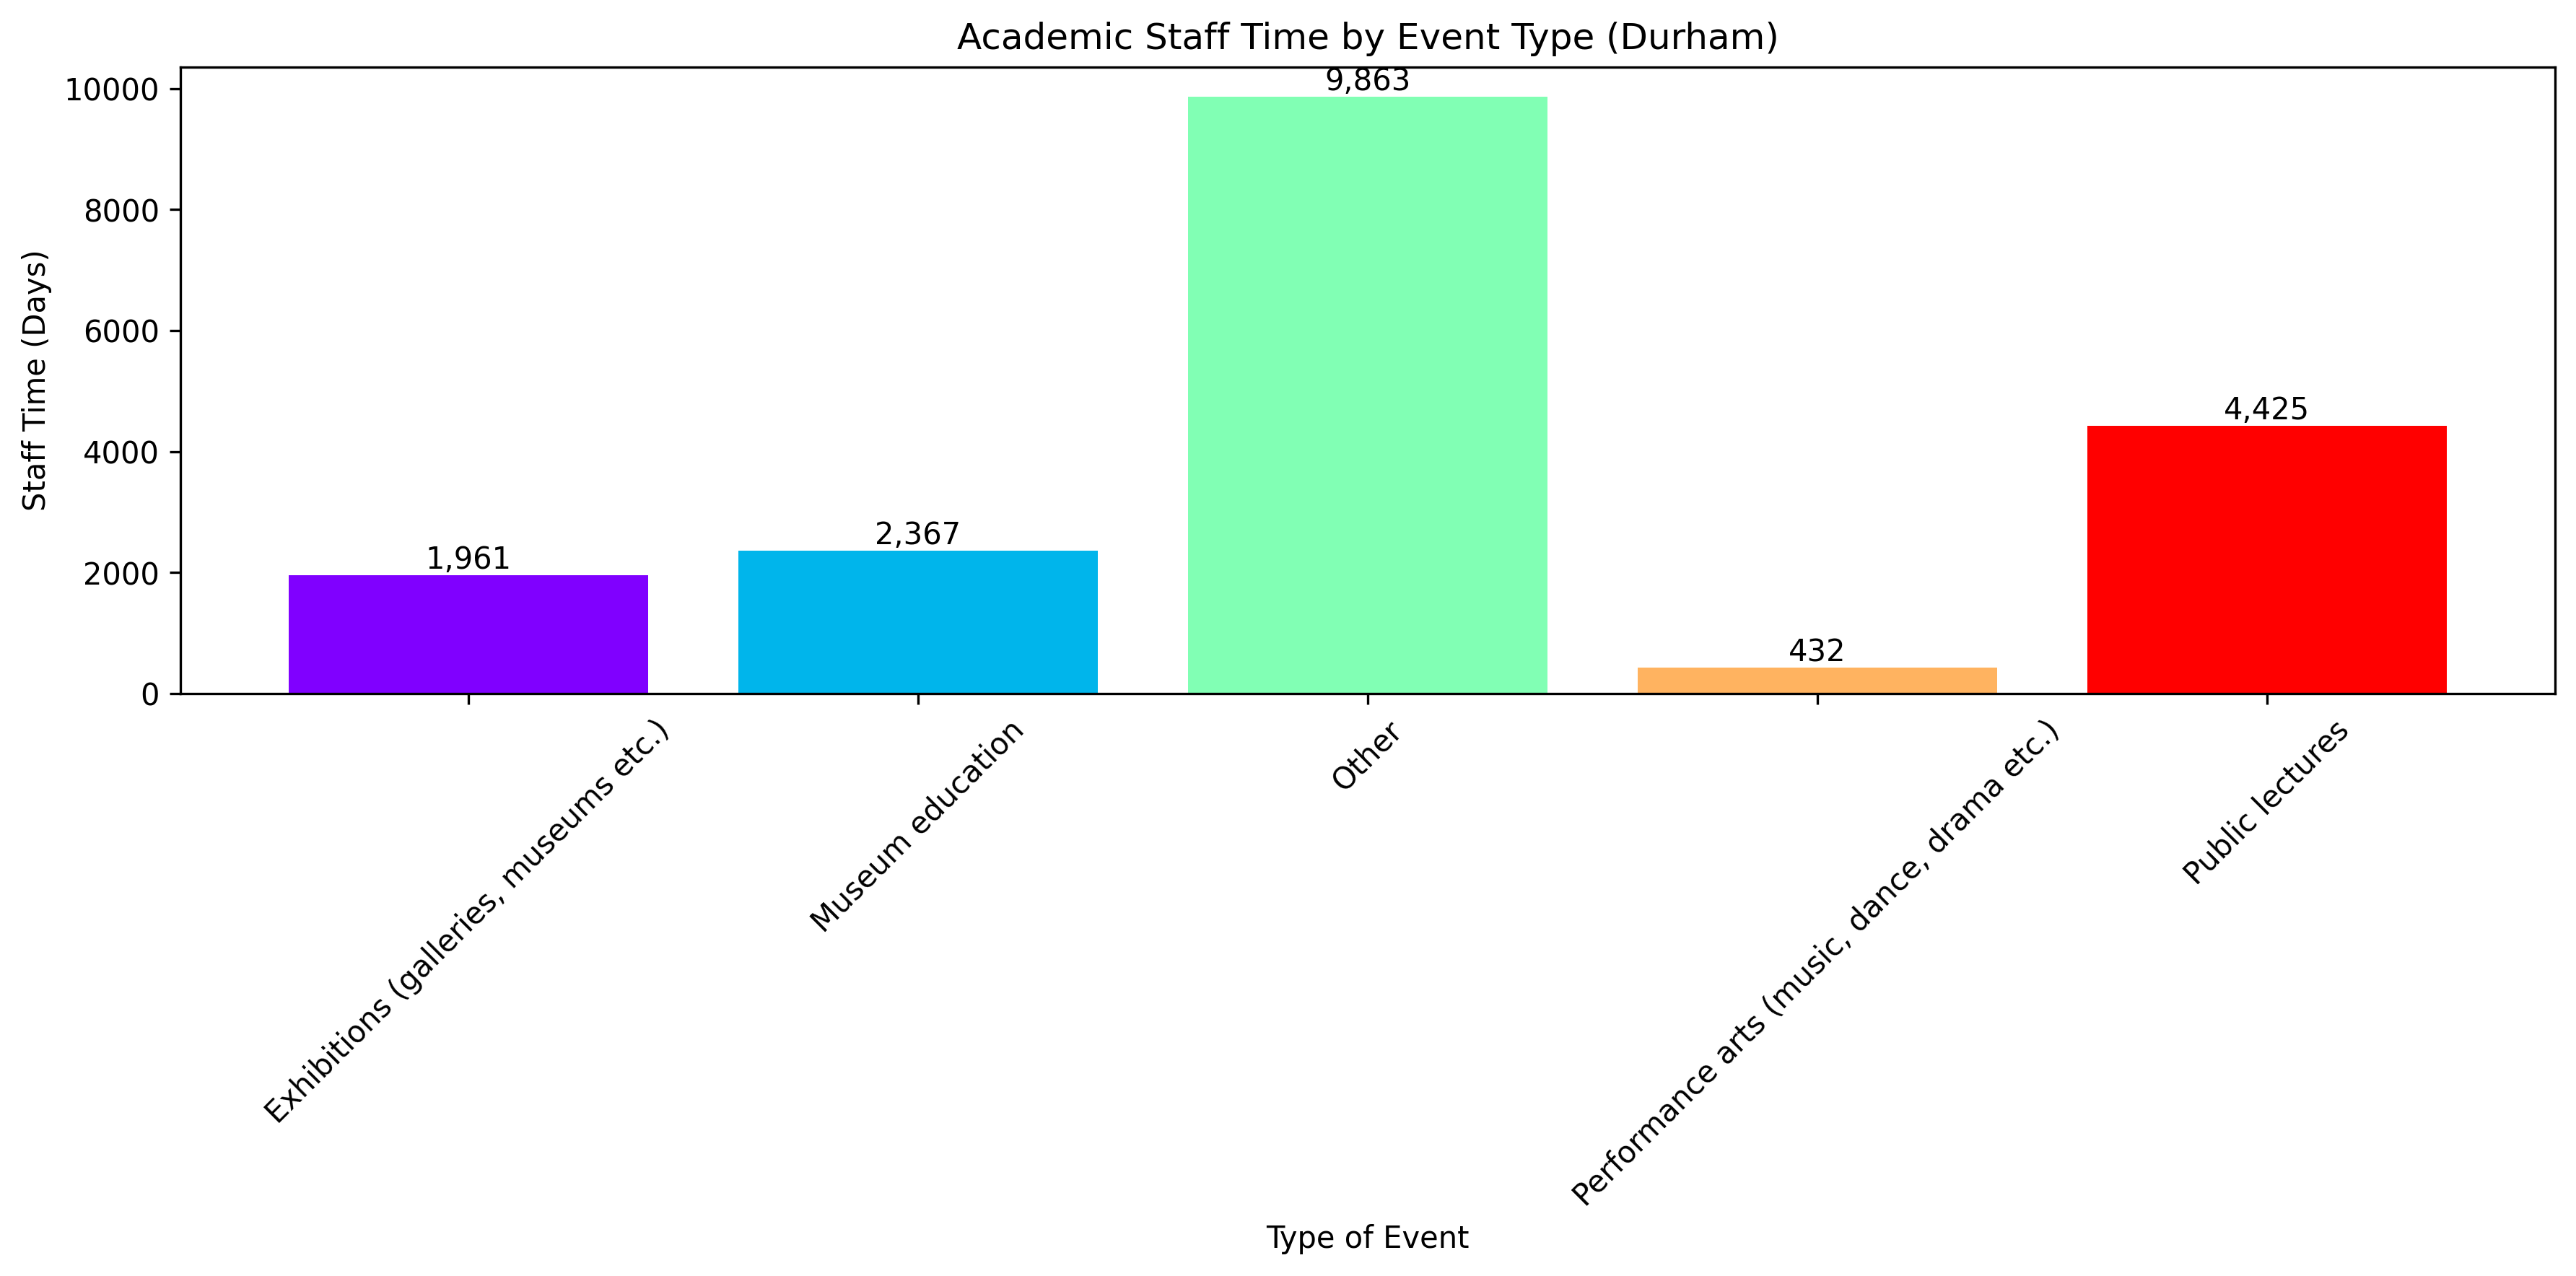
\includegraphics[width=\textwidth]{Fig/figure33.staff_time_by_type.png}
    \caption{Type of staff time}
    \label{fig:staff-time-by-type}
\end{subfigure}
\vspace{0.6cm}
\caption{Participation Analysis}
\label{fig:participation-analysis}
\end{figure}

Durham's public engagement strategy benefits from significant audience reach and academic involvement. The strong alignment between event type popularity and staff time allocation reflects efficient and strategic resource use in community-facing activities.

\subsubsection{Regional Comparison}

Durham ranks second in the North East for total engagement events (6,043,792), closely following Newcastle University (7,181,816) and well ahead of Northumbria (1,208,122), Sunderland (754,978), and Teesside (273,150).

This close performance with Newcastle and clear lead over other regional institutions highlights Durham's prominent role in the region's cultural and educational landscape. Its sustained engagement levels reinforce its importance as a major hub of public interaction in the North East.



Durham maintains a leading regional presence in public engagement. Its near-parity with Newcastle University and substantial lead over other regional institutions affirm its standing as a cornerstone of community engagement and outreach in the region.

\begin{figure}[h]
\centering
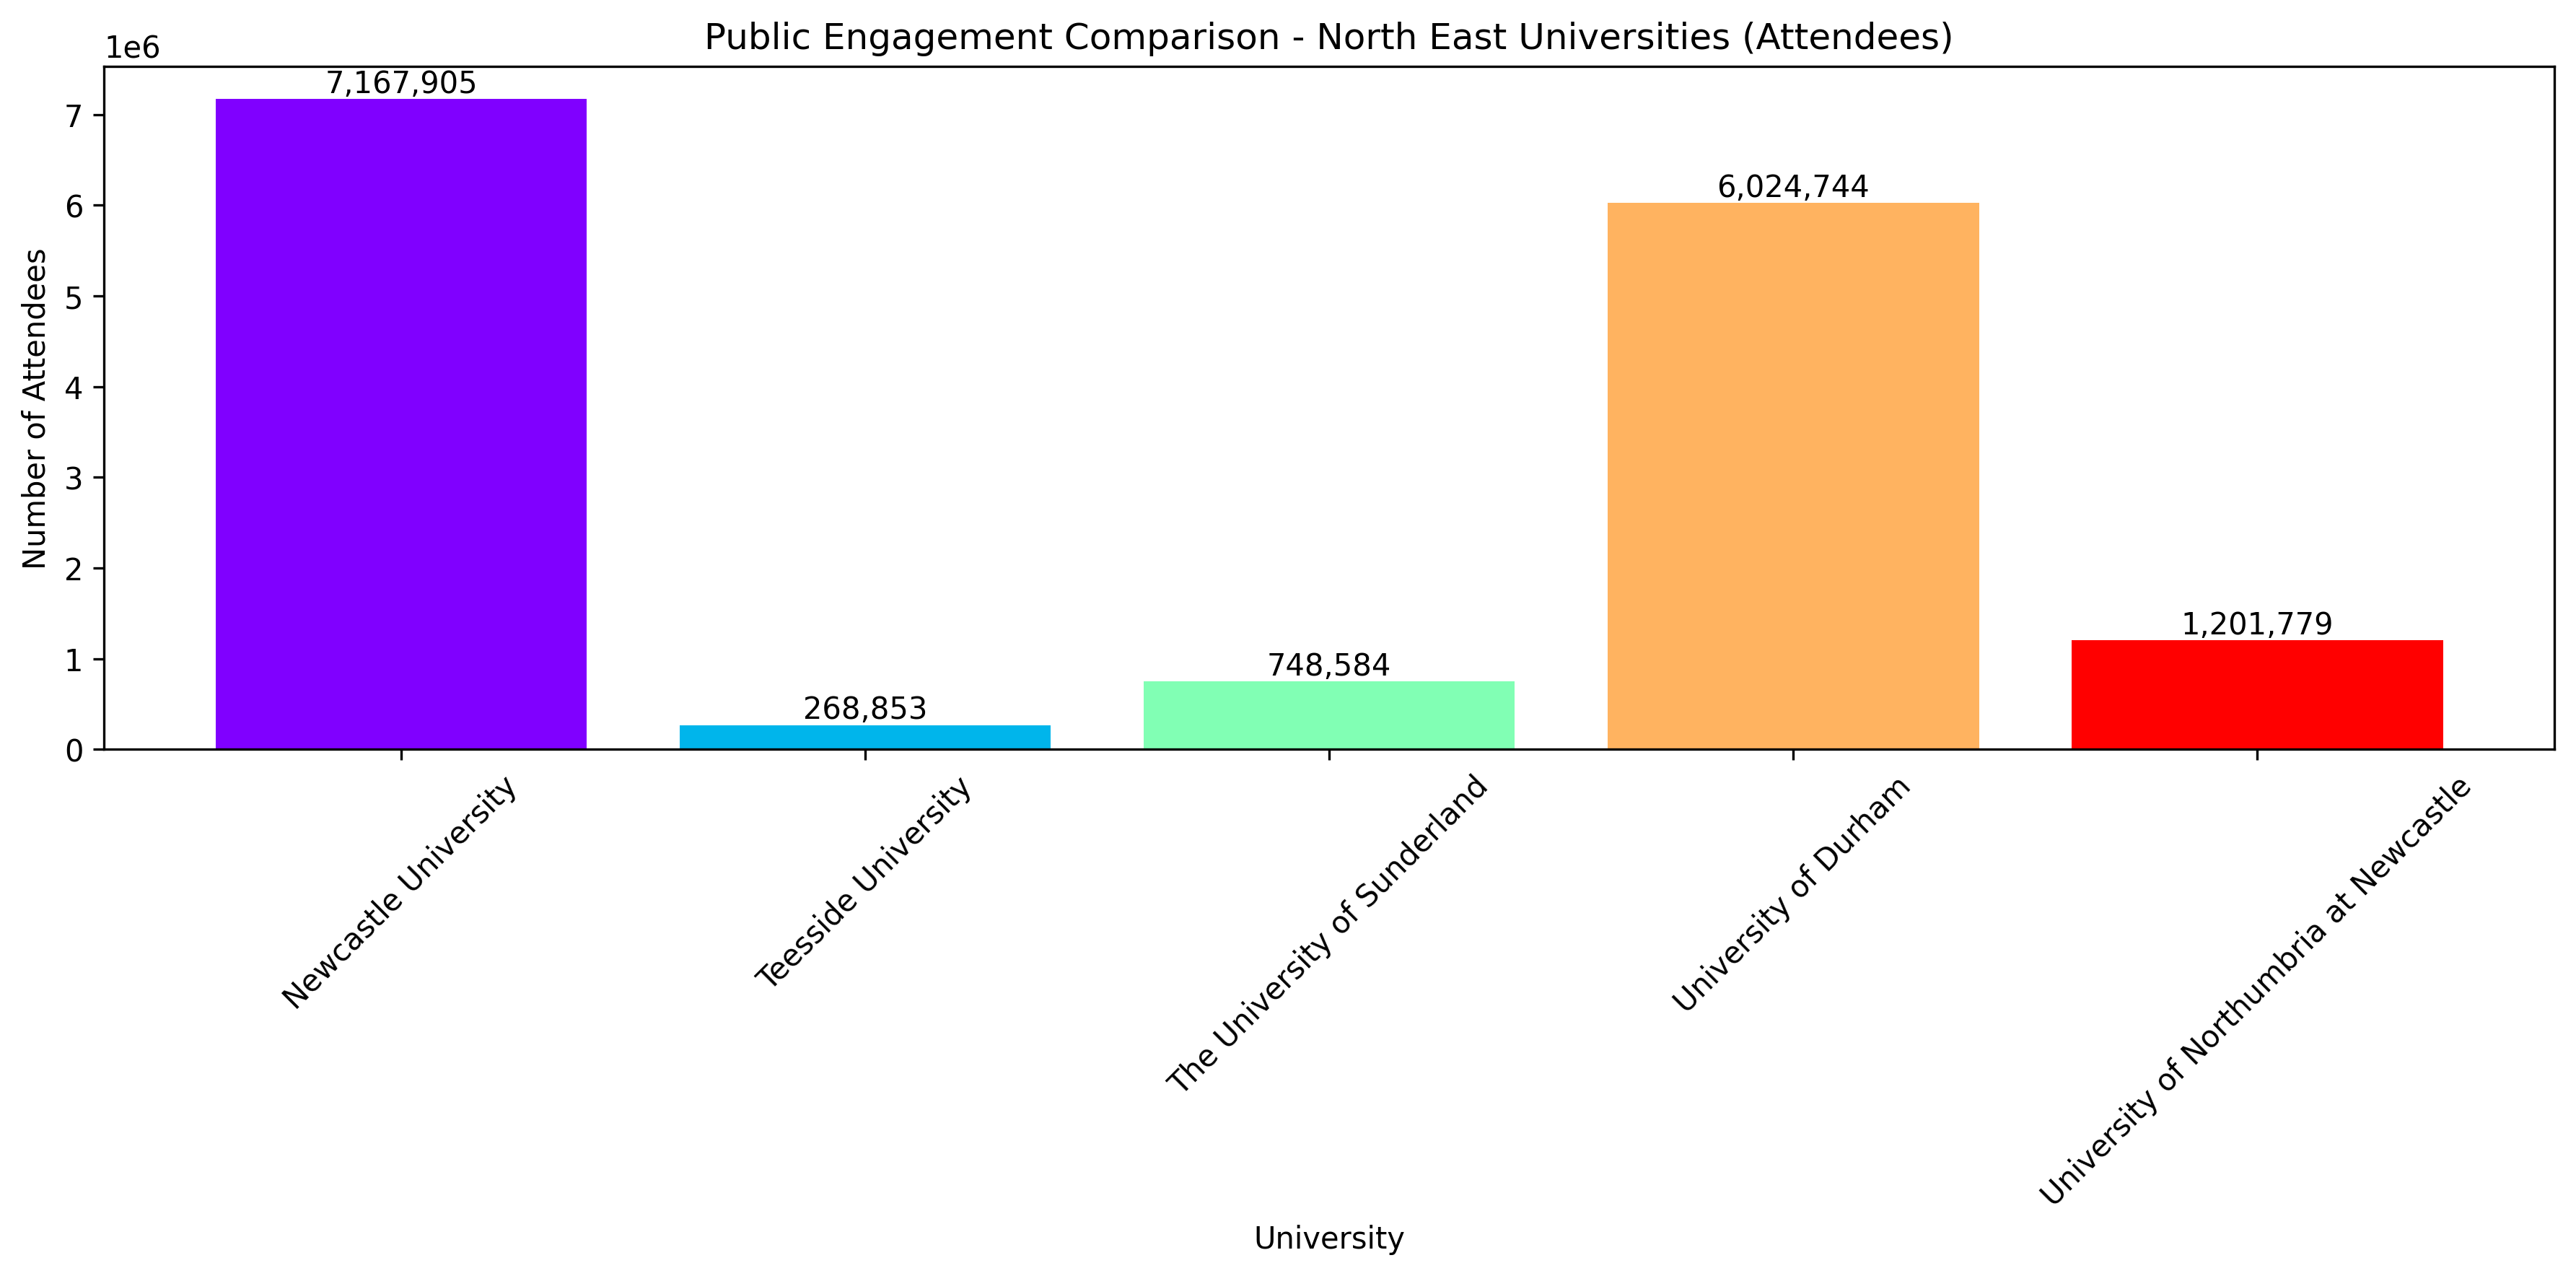
\includegraphics[width=0.8\textwidth]{Fig/figure34.ne_comparison.png}
\caption{Public Engagement NE comparison - Total Events}
\label{fig:ne-comparison}
\end{figure}

Durham maintains a leading regional presence in public engagement. Its near-parity with Newcastle University and substantial lead over other regional institutions affirm its standing as a cornerstone of community engagement and outreach in the region.

\subsubsection{Overall Public Engagement Performance}

Durham University's public engagement performance demonstrates both breadth and depth. While total engagement numbers fall below the national average, the university excels within the North East, driven by high event diversity, a large share of free programming, and meaningful academic involvement. The strategic allocation of staff time and commitment to inclusive outreach underscore Durham's strong institutional support for public engagement as a core mission area. Public engagement analysis demonstrates Durham University's commitment to community involvement, with a total engagement value of \textsterling 6,043,792. The university's approach is characterized by a strong focus on free events (72.1\% of total events) and diverse programming, including exhibitions, public lectures, and museum education. With 6,024,744 total attendees and 19,048 days of academic staff involvement, the university shows significant community impact. While ranking 31st nationally, the university maintains a strong second position in the North East region, closely following Newcastle University.

\subsection{Regional and Specialization Analysis}
\label{sec:regional-analysis}

\subsubsection{Regional Ranking Analysis}

\begin{itemize}
    \item \textbf{Research Income Rankings:} Durham University holds the second-highest position in the North East region for research income, following Newcastle University. It leads ahead of Northumbria, Teesside, and Sunderland, consistently reinforcing its position as a top research institution in the region.
    
    \item \textbf{Business Income Rankings:} In business services income, Durham also ranks second, again following Newcastle. It outperforms Teesside, Northumbria, and Sunderland, indicating a solid standing in university-industry engagement and consultancy services within the region.
    
    \item \textbf{IP Performance Rankings:} Durham consistently ranks third in IP disclosures across the North East, following Newcastle and Northumbria. While its rank for IP income and licenses fluctuates between second and fourth place, it remains within the top tier, signaling strong overall performance in intellectual property activity, albeit with room to enhance income conversion.
\end{itemize}

Durham University maintains a strong and stable regional profile, consistently ranking second in research income and business services, and third in IP disclosures. Its solid performance across these metrics underscores its growing influence and leadership potential within the North East higher education landscape.


\begin{figure}[h]
\centering
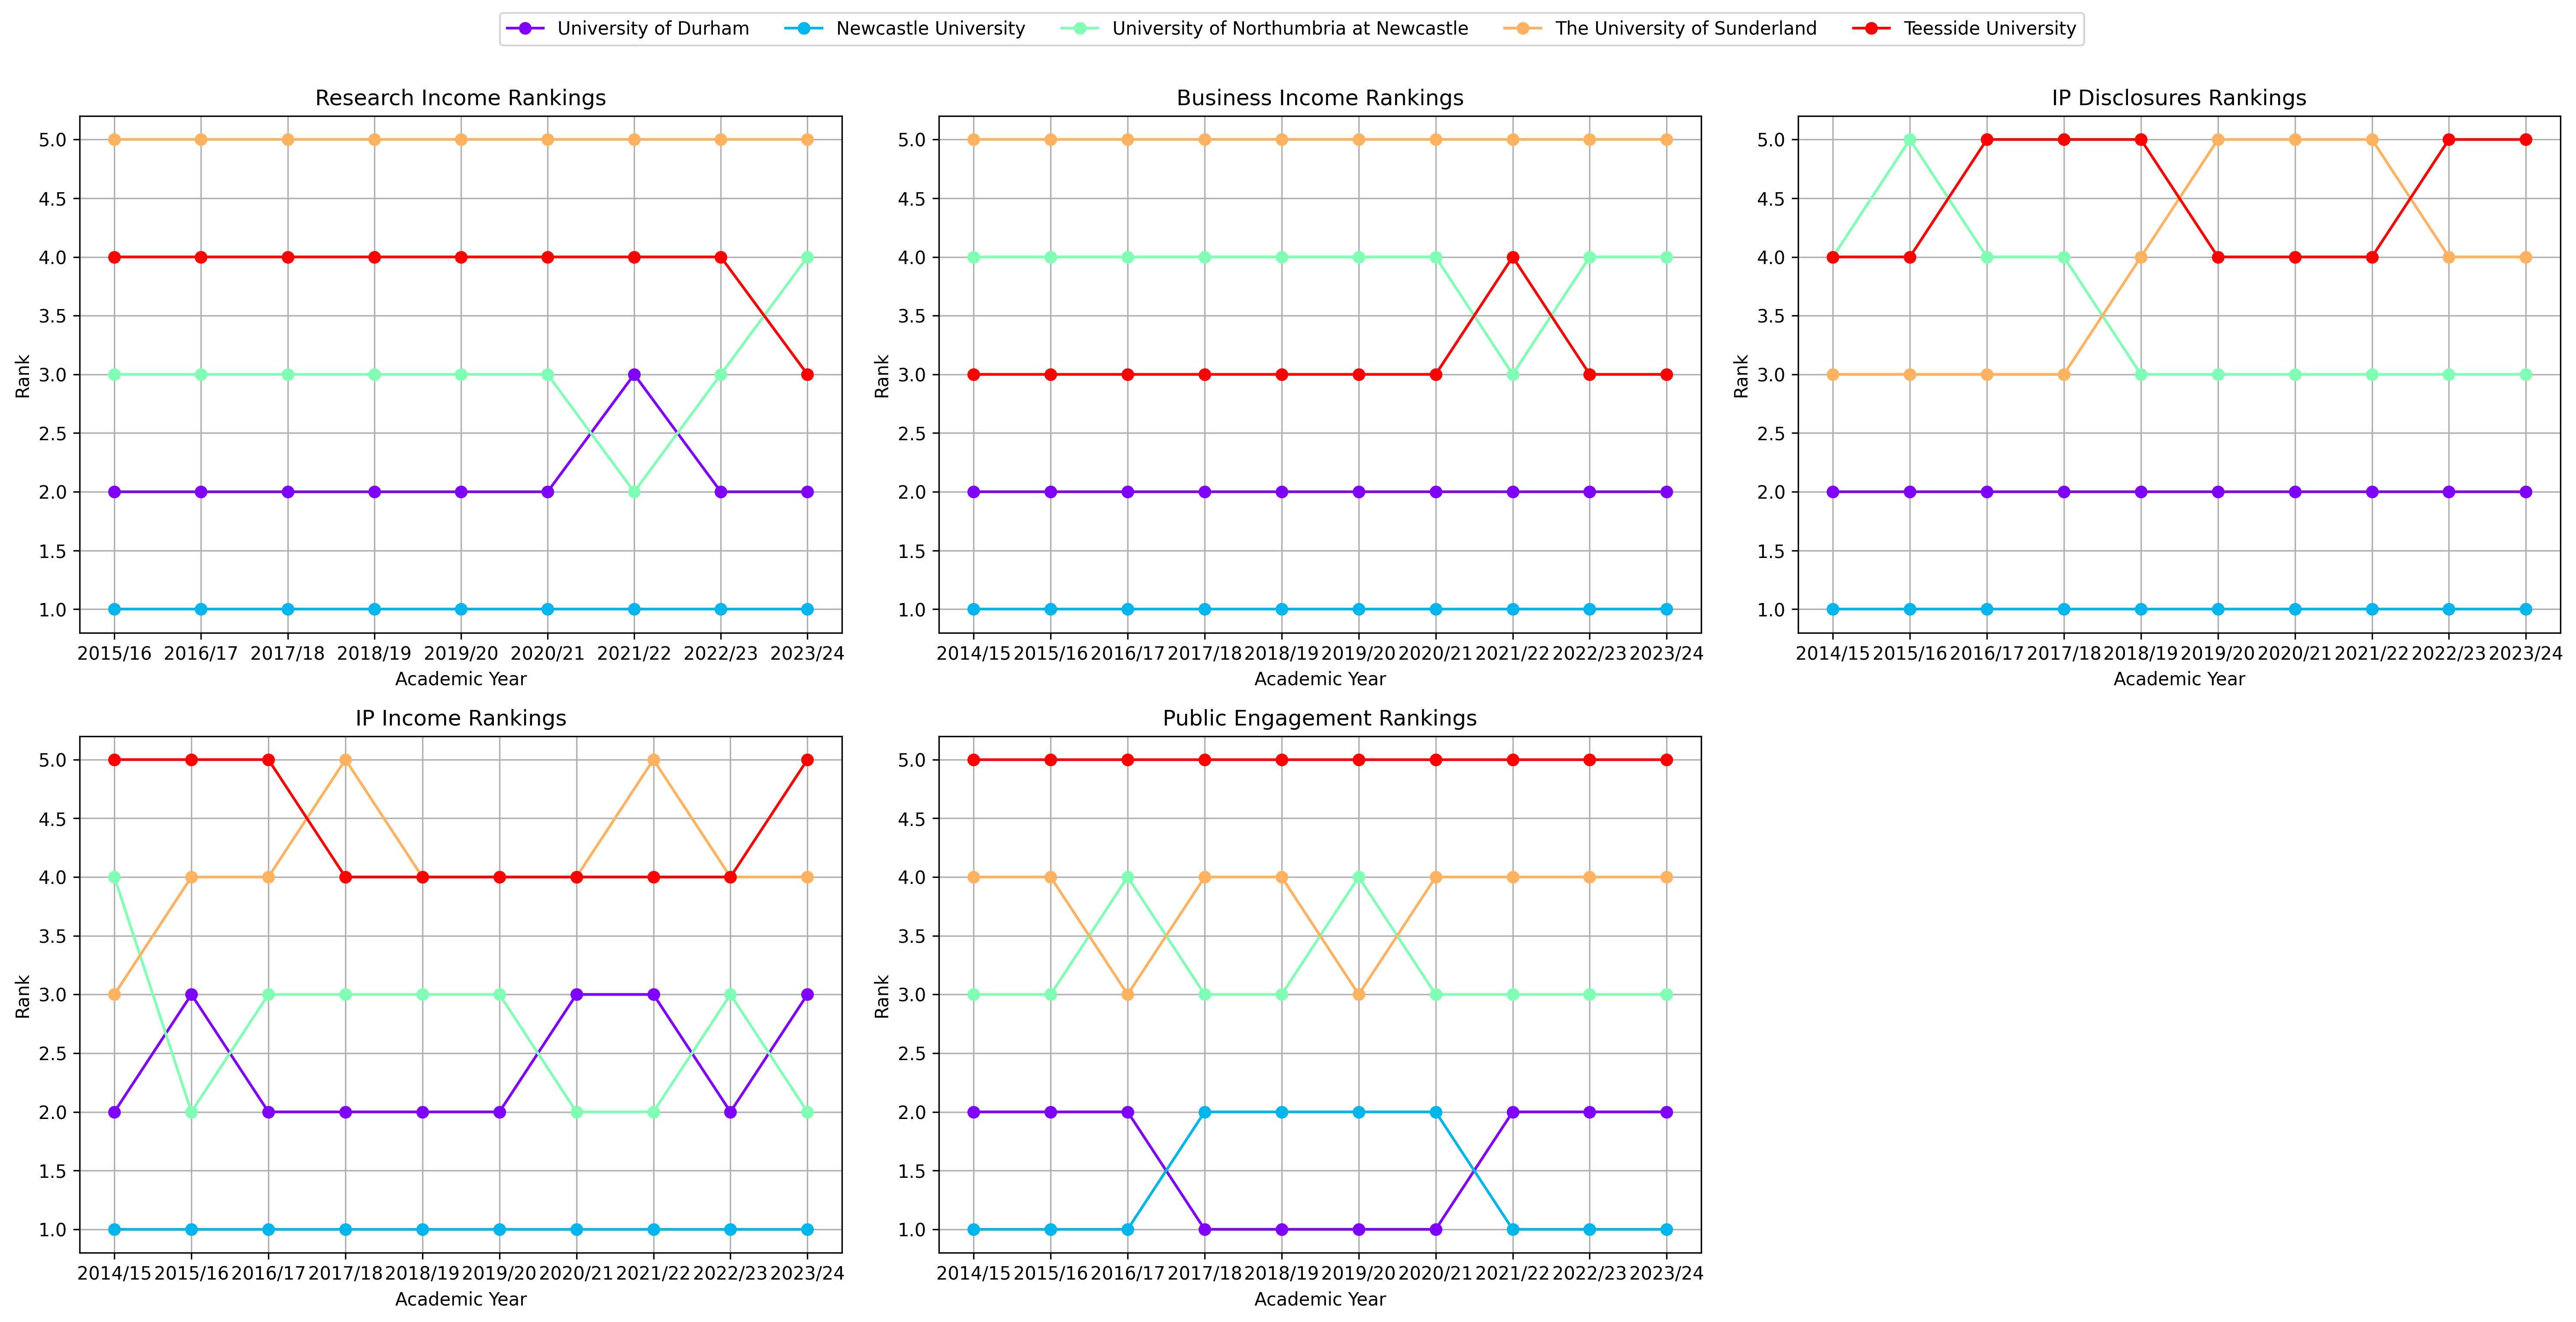
\includegraphics[width=0.99\textwidth]{Fig/figure35.ranking_changes.png}
\caption{Ranking changes}
\label{fig:ranking-changes}
\end{figure}

\subsubsection{Correlation Matrix of Key Metrics}

To better understand the structural factors behind Durham's strong and multi-dimensional performance, a correlation matrix, based on the work of Pearson (1895) \cite{pearson1895notes} and Fisher (1915) \cite{fisher1915frequency}, was generated to examine relationships among key metrics. The matrix reveals that research income is strongly correlated with business income ($\mathrm{r}=0.87$) and IP disclosures ($\mathrm{r}=0.83$), while business income also shows a high correlation with IP disclosures ($\mathrm{r}=0.88$) and public engagement ($\mathrm{r}=0.72$). These positive correlations suggest that institutions with strong research capability tend to excel in commercialization and engagement activities as well. Durham's sustained performance across all these metrics may thus reflect an integrated institutional ecosystem, where research, industry collaboration, and public outreach are mutually reinforcing. This structural alignment provides a solid foundation for its regional competitiveness.



\begin{figure}[h]
\centering
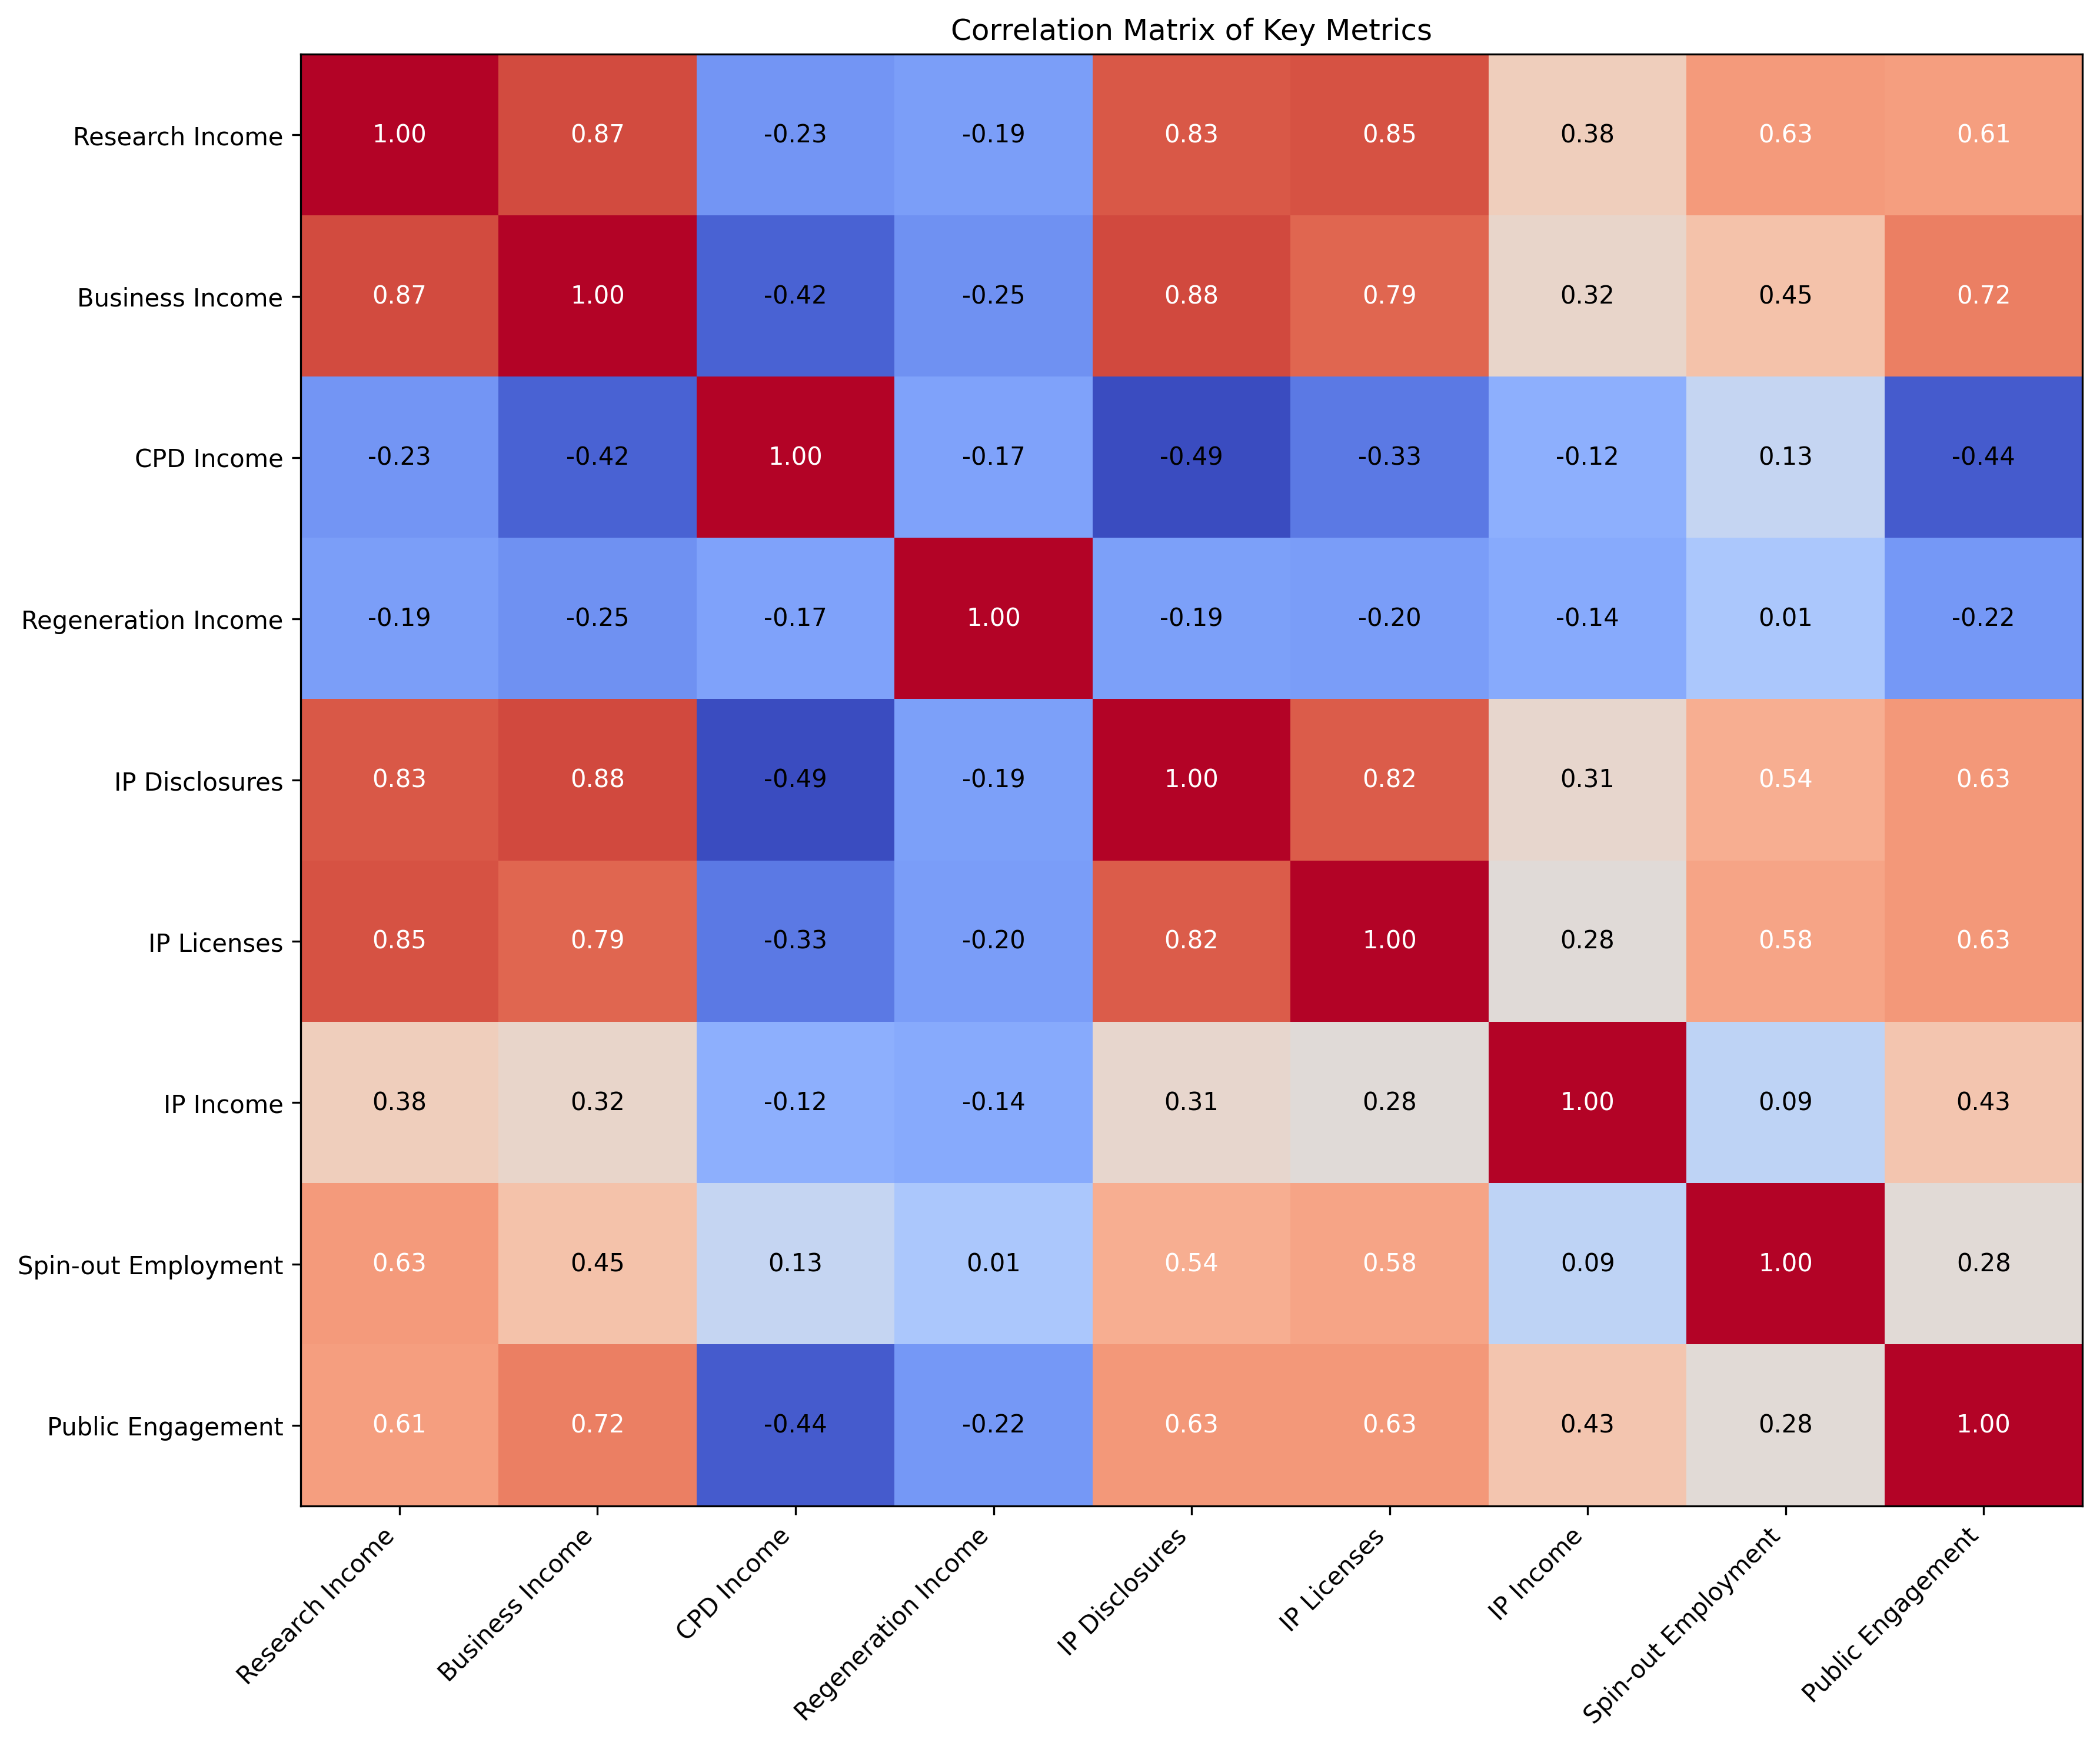
\includegraphics[width=0.6\textwidth]{Fig/figure36.correlation_matrix.png}
\caption{Correlation Matrix of Key metrics}
\label{fig:correlation-matrix}
\end{figure}

\subsubsection{Specialization Analysis}

\begin{itemize}
    \item \textbf{Research Specialization (HHI):} Durham demonstrates a moderate level of research specialization\footnote{Research specialization HHI measures the concentration of research activities across different research fields or funding sources, where lower values indicate better diversification across research areas.}, as described by Porter (1985) \cite{porter1985competitive}, with HHI values ranging from 0.28 to 0.31, similar to peers like Newcastle and Northumbria. These figures suggest a well-diversified research base, with no overconcentration in a narrow set of fields.

\item \textbf{Business Services Specialization:} The university shows higher business services specialization\footnote{Business services specialization HHI measures the concentration of business service activities across different service types, where higher values indicate greater focus on specific service areas.}, with HHI values between 0.47 and 0.69. This indicates that certain service areas dominate income streams, offering opportunities for targeted growth but also posing concentration risks that may require strategic diversification.

\item \textbf{IP Specialization:} Durham's IP specialization index\footnote{IP specialization HHI measures the concentration of intellectual property activities across different IP types or commercialization channels, where higher values indicate greater focus on specific IP areas.} varies from 0.27 to 0.62, reflecting increasing focus on select IP areas, as outlined by Teece (1986) \cite{teece1986profiting}. While this may enhance strength in particular technologies or domains, it also calls for careful portfolio management to avoid overreliance on limited segments.

\item \textbf{Public Engagement Specialization:} Durham's public engagement activities show significant variation in specialization\footnote{Public engagement specialization HHI measures the concentration of public engagement activities across different event types or engagement categories, where higher values indicate greater focus on specific engagement areas.}, with HHI values ranging from 0.27 to 0.89, averaging 0.59. This indicates periods of both high diversification (2014/15, 2015/16) and high concentration (2017/18-2019/20), suggesting evolving engagement strategies that may reflect changing institutional priorities or external factors such as the COVID-19 pandemic impact on event types.
\end{itemize}


\begin{figure}[h]
\centering
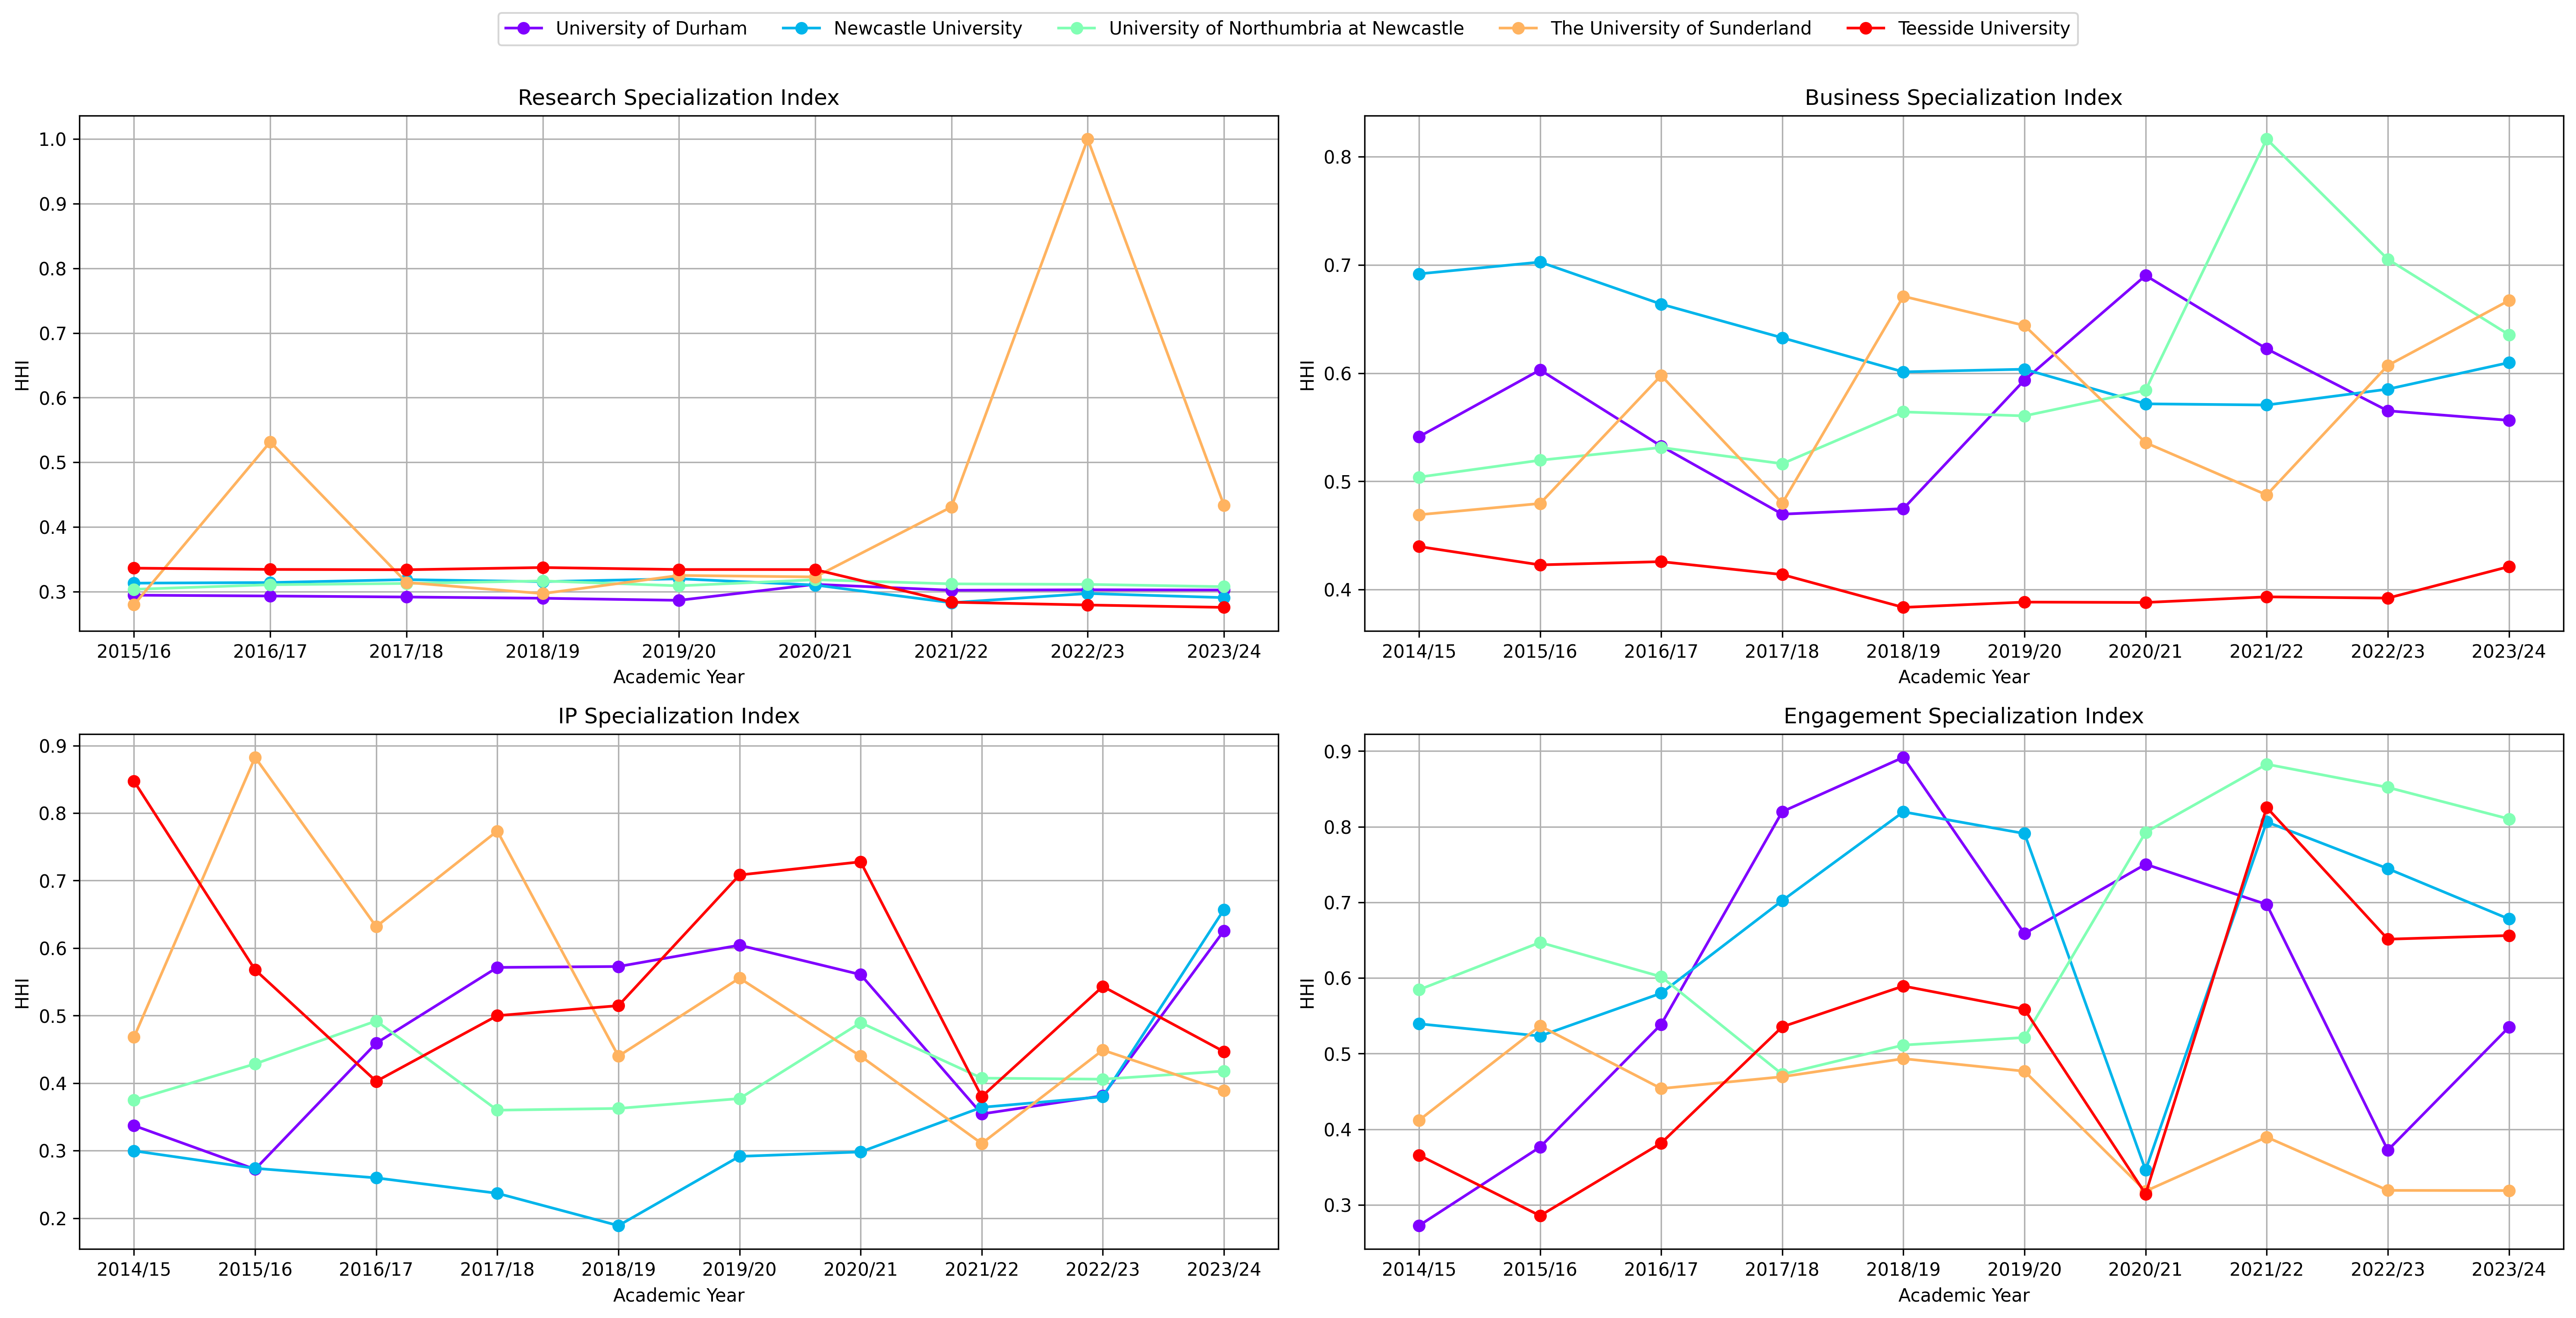
\includegraphics[width=0.99\textwidth]{Fig/figure37.specialization_indices.png}
\caption{Specialization indices}
\label{fig:specialization-indices}
\end{figure}

Durham displays a strategically balanced specialization profile. Its research activity is well diversified, while its business services and IP activities show signs of increasing focus. Public engagement activities demonstrate the highest variability in specialization patterns, reflecting adaptive strategies in response to changing circumstances. This combination supports both broad academic engagement and the development of specialized expertise, though greater diversification in IP monetization could improve resilience and impact. As illustrated in Figure~\ref{fig:specialization-indices}, Durham's HHI values demonstrate balanced diversification across research domains while maintaining focused expertise in business services and variable engagement strategies.

\subsubsection{Regional Position Analysis}

Based on the comprehensive ranking analysis presented in Figure~\ref{fig:ranking-changes} and the correlation patterns shown in Figure~\ref{fig:correlation-matrix}, Durham University's regional positioning can be characterized as follows:

\begin{itemize}
    \item \textbf{Overall Regional Standing:} Durham ranks second in the North East for research income and business income, third in IP disclosures, and places among the top two in public engagement (ranking first in most years, second in 2017/18-2020/21). These consistently high standings across multiple domains reinforce its influence in the regional academic ecosystem.
    
    \item \textbf{Competitive Position:} The university's main regional competitor is Newcastle University, which it closely trails in several areas. Durham maintains a significant lead over other local institutions (Northumbria, Teesside, and Sunderland), reflecting its robust capabilities and multi-dimensional performance.
    
    \item \textbf{Regional Leadership:} Durham's consistent top-tier performance, particularly in research and public engagement, positions it as a regional leader. Its balanced portfolio enables it to engage effectively across education, industry, and society, providing a strong platform for sustained regional influence.
\end{itemize}

As demonstrated in the ranking analysis data (generated by script 5.extral\_regional\_analysis.py), Durham University demonstrates strong competitive standing within the North East, consistently performing among the top two institutions across key indicators. Its comprehensive strength in research, business engagement, and public service highlights its role as a key driver of regional development and innovation.

\subsubsection{Overall Regional and Specialization Performance}

Durham University's regional and specialization analysis reveals a resilient and balanced institutional profile. Its consistent second-place ranking in research and business activities, and third-place ranking in IP disclosures across the North East indicates a dependable regional presence. The university maintains a diversified research base and a more focused approach in business services, with growing concentration in certain IP areas. While it performs well in IP generation, there are opportunities to enhance commercialization outcomes. Overall, Durham's strong regional performance and thoughtful specialization strategy offer a solid foundation for long-term growth and leadership within the region, with further potential in IP income generation and service diversification. The regional and specialization analysis reveals Durham University's strong position in the North East region, consistently ranking second in research and business metrics, and third in IP disclosures. The university demonstrates a balanced approach to specialization, with moderate HHI values in research (0.28-0.32) indicating good diversification. Business services show higher specialization (0.47-0.69), suggesting focused expertise in particular areas. The analysis highlights the university's competitive advantages in research and public engagement, while identifying opportunities for improvement in IP commercialization and business services diversification.

\subsection{Performance Efficiency Analysis}
\label{sec:performance-efficiency}

This section evaluates how effectively North East universities convert their academic staff time into income-generating activities across four key domains: research, business services, intellectual property, and continuing professional development (CPD), as established by Johnes (2006) \cite{johnes2006data} and Worthington (2001) \cite{worthington2001empirical}. The analysis quantifies efficiency as the amount of income earned per academic staff day, providing a normalized metric for inter-institutional comparison.

\subsubsection{North East University Efficiency Comparison}

Across all four domains, Newcastle University leads in research and IP efficiency, while Teesside University excels in CPD efficiency. Durham University, despite its strong total income, shows comparatively lower efficiency figures across most domains, particularly in CPD monetization. The detailed average efficiency values are summarized in Table~\ref{tab:efficiency-comparison}.
\vspace{0.25cm}
\begin{table}[h]
\centering
\caption{North East University Efficiency Comparison}
\vspace{0.1cm}
\resizebox{0.9\textwidth}{!}{%
\begin{tabular}{|l|l|l|l|l|}
\hline \textbf{University} & \textbf{Research Efficiency (\textsterling/staff day)} & \textbf{Business Efficiency (\textsterling/staff day)} & \textbf{IP Efficiency (\textsterling/staff day)} & \textbf{CPD Efficiency (\textsterling/staff day)} \\
\hline Newcastle University & \textsterling 117.35 & \textsterling 64.44 & \textsterling 3.02 & \textsterling 2.21 \\
\hline Teesside University & \textsterling 46.53 & \textsterling 43.84 & \textsterling 0.01 & \textsterling 31.56 \\
\hline University of Northumbria at Newcastle & \textsterling 39.21 & \textsterling 13.78 & \textsterling 0.11 & \textsterling 15.92 \\
\hline University of Durham & \textsterling 19.76 & \textsterling 27.73 & \textsterling 0.44 & \textsterling 0.64 \\
\hline The University of Sunderland & \textsterling 0.78 & \textsterling 4.82 & \textsterling 0.02 & \textsterling 3.09 \\
\hline
\end{tabular}
}
\label{tab:efficiency-comparison}
\end{table}

\subsubsection{Efficiency Analysis by Domain}

\begin{itemize}
    \item \textbf{Research Efficiency:} Newcastle University far outperforms all others with \textsterling 117.4 per staff day. Teesside (\textsterling 46.5) and Northumbria (\textsterling 39.2) follow, while Durham ranks fourth at \textsterling 19.8. Sunderland lags significantly at \textsterling 0.78 per staff day, suggesting low conversion of staff input into research income.
    
    \item \textbf{Business Services Efficiency:} Newcastle again leads at \textsterling 64.4, followed by Teesside (\textsterling 43.8). Durham generates \textsterling 27.7 per staff day in this domain, indicating moderate engagement. Sunderland's figure of \textsterling 4.8 underscores minimal business service impact.
    
    \item \textbf{IP Efficiency:} All universities show low performance here. Newcastle is the only institution exceeding \textsterling 2.0 (\textsterling 3.0 per staff day), while Durham shows \textsterling 0.44 per staff day and the rest remain below \textsterling 0.12. This suggests that despite patent filings or licenses, direct financial returns from IP remain limited regionally.
    
    \item \textbf{CPD Efficiency:} Teesside University leads significantly with \textsterling 31.6 per staff day, followed by Northumbria (\textsterling 15.9) and Sunderland (\textsterling 3.1). Newcastle (\textsterling 2.2) and Durham (\textsterling 0.6) show relatively low CPD efficiency, indicating substantial room for improvement in professional development monetization.
\end{itemize}

\subsubsection{Efficiency Trends Analysis}

The efficiency trends analysis reveals the annual growth patterns across different income domains, providing insights into the long-term performance trajectory of North East universities. Table~\ref{tab:efficiency-trends} presents the trend analysis results, showing the annual efficiency growth rates in GBP per staff day.

\begin{table}[h]
\centering
\caption{Efficiency Trends Analysis - North East Universities (GBP per staff day per year)}
\vspace{0.1cm}
\resizebox{0.9\textwidth}{!}{%
\begin{tabular}{|l|l|l|l|l|}
\hline \textbf{University} & \textbf{Research Trend} & \textbf{Business Trend} & \textbf{IP Trend} & \textbf{CPD Trend} \\
\hline Newcastle University & +4.15 & +2.13 & -0.03 & +0.07 \\
\hline University of Durham & +4.60 & +3.00 & -0.02 & +0.13 \\
\hline University of Northumbria at Newcastle & +8.28 & +2.10 & +0.02 & +1.47 \\
\hline Teesside University & +19.17 & +8.37 & +0.00 & +7.96 \\
\hline The University of Sunderland & -0.02 & +0.38 & +0.00 & +0.22 \\
\hline
\end{tabular}
}
\label{tab:efficiency-trends}
\end{table}

As shown in Table~\ref{tab:efficiency-trends}, Durham University demonstrates positive efficiency trends across all domains, with particularly strong growth in research efficiency (+4.60 GBP/year) and business efficiency (+3.00 GBP/year). Teesside University shows the most impressive growth rates, particularly in research (+19.17 GBP/year) and CPD (+7.96 GBP/year) efficiency. Newcastle University maintains steady but moderate growth across all domains, while Sunderland shows minimal growth, particularly in research efficiency where it shows a slight decline (-0.02 GBP/year).

The trend analysis reveals that Durham's efficiency improvements are consistent but modest compared to regional leaders. While the university shows positive momentum across all income streams, the growth rates suggest that more aggressive efficiency optimization strategies may be needed to close the gap with top-performing institutions. The efficiency trends are visualized in Figure~\ref{fig:efficiency-trends}.



\begin{figure}[h]
\centering
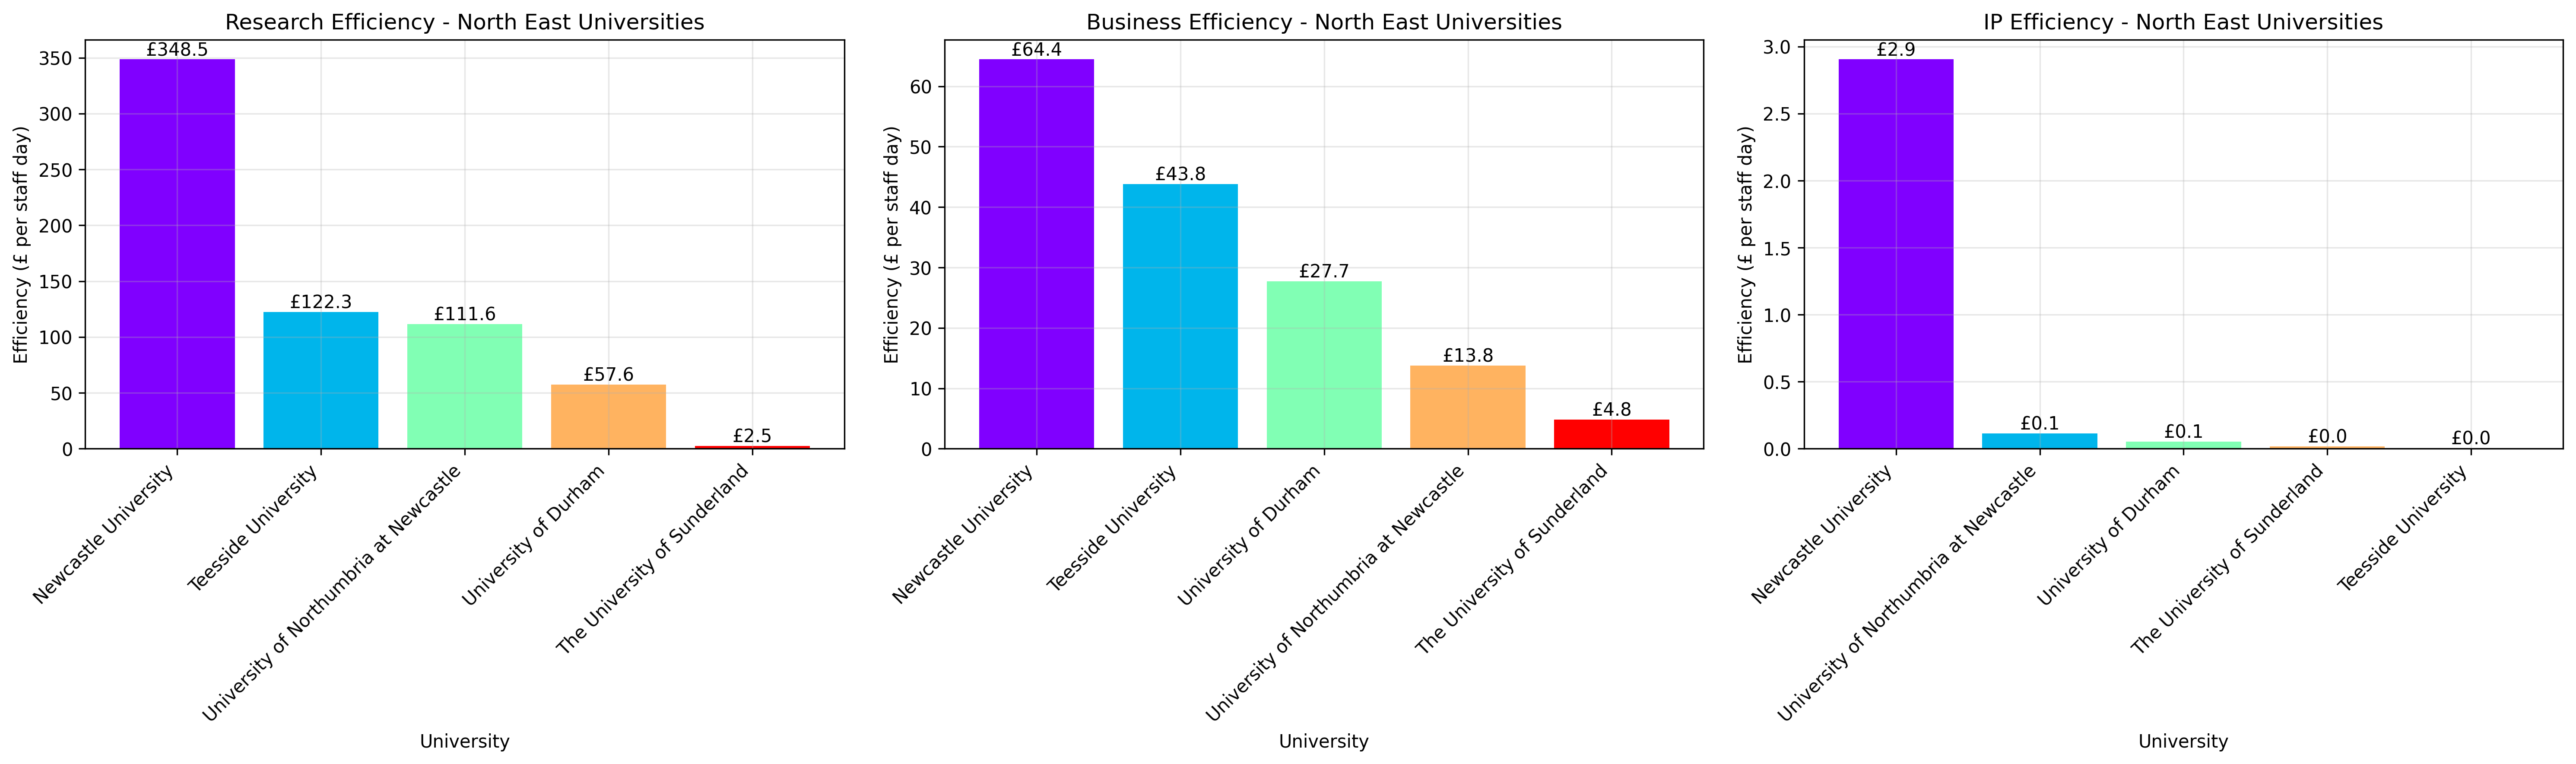
\includegraphics[width=0.99\textwidth]{Fig/figure38.ne_efficiency_comparison.png}
\caption{Average Efficiency by Domain - North East Universities}
\label{fig:ne-efficiency-comparison}
\end{figure}

These results highlight a clear efficiency gap between Newcastle and the rest of the North East institutions, particularly in high-value domains like research and IP. Durham University, while producing strong total outputs (as shown in previous sections), shows relatively modest returns per unit of staff time. Figure~\ref{fig:ne-efficiency-comparison} illustrates the efficiency gap between Newcastle and other regional institutions, highlighting Durham's competitive positioning.

\subsubsection{Temporal Trends in Efficiency}

\begin{itemize}
    \item \textbf{Research:} Newcastle's research efficiency peaked in 2019/20 at over \textsterling 750 per staff day before gradually declining—likely influenced by funding cycles and COVID-19 disruptions. Durham shows gradual improvement from 2019/20 onward, closing the gap with Northumbria and Teesside by 2023/24.
    
    \item \textbf{Business:} Teesside's business efficiency exhibits volatility but rises sharply in recent years (100.1 in 2023/24). Durham shows steady improvement post-2020. Northumbria remains stable, while Sunderland and Newcastle display moderate fluctuations.
    
    \item \textbf{IP:} IP efficiency remains low and unstable for all universities. Newcastle again leads but with notable peaks and troughs, while others show near-zero efficiency with little temporal improvement.
\end{itemize}

\begin{figure}[h]
\centering
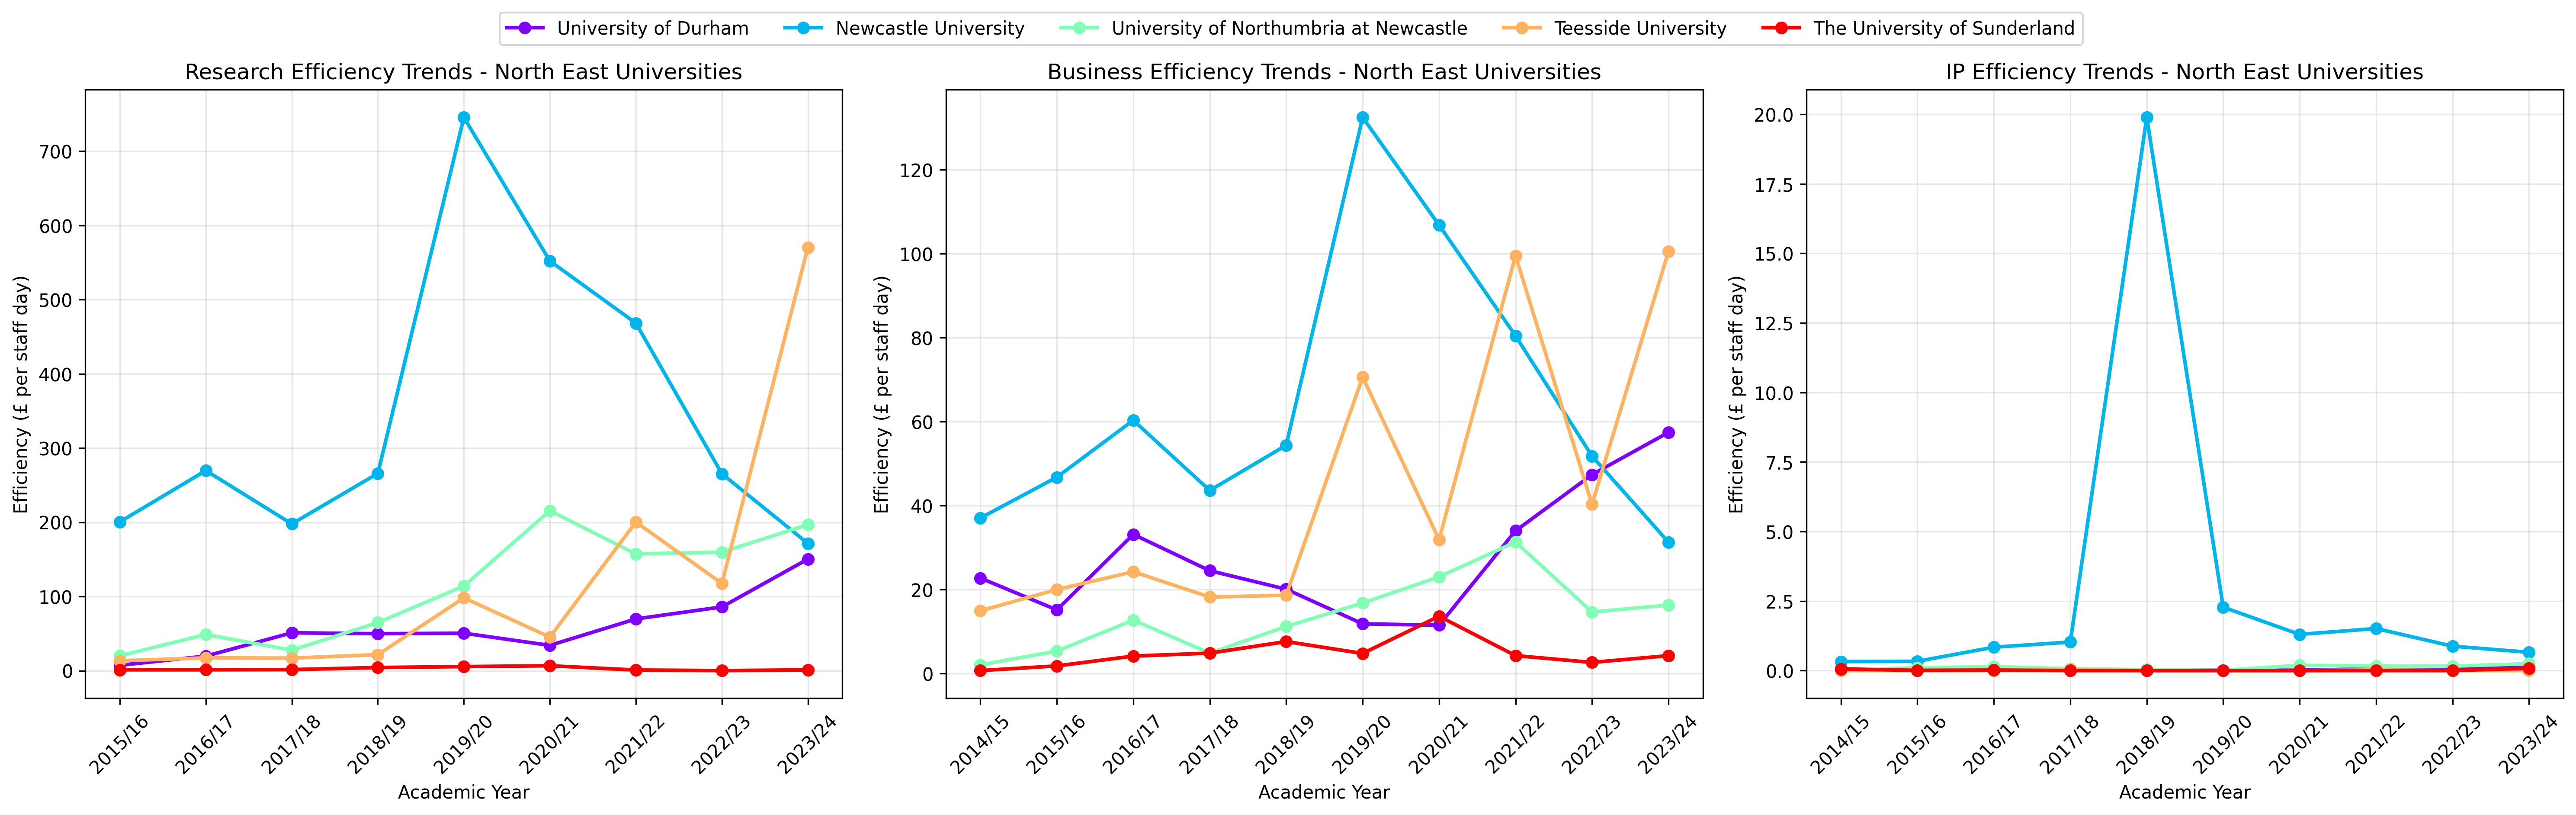
\includegraphics[width=0.99\textwidth]{Fig/figure39.efficiency_trends.png}
\caption{Efficiency Trends over Time}
\label{fig:efficiency-trends}
\end{figure}

\begin{figure}[h]
\centering
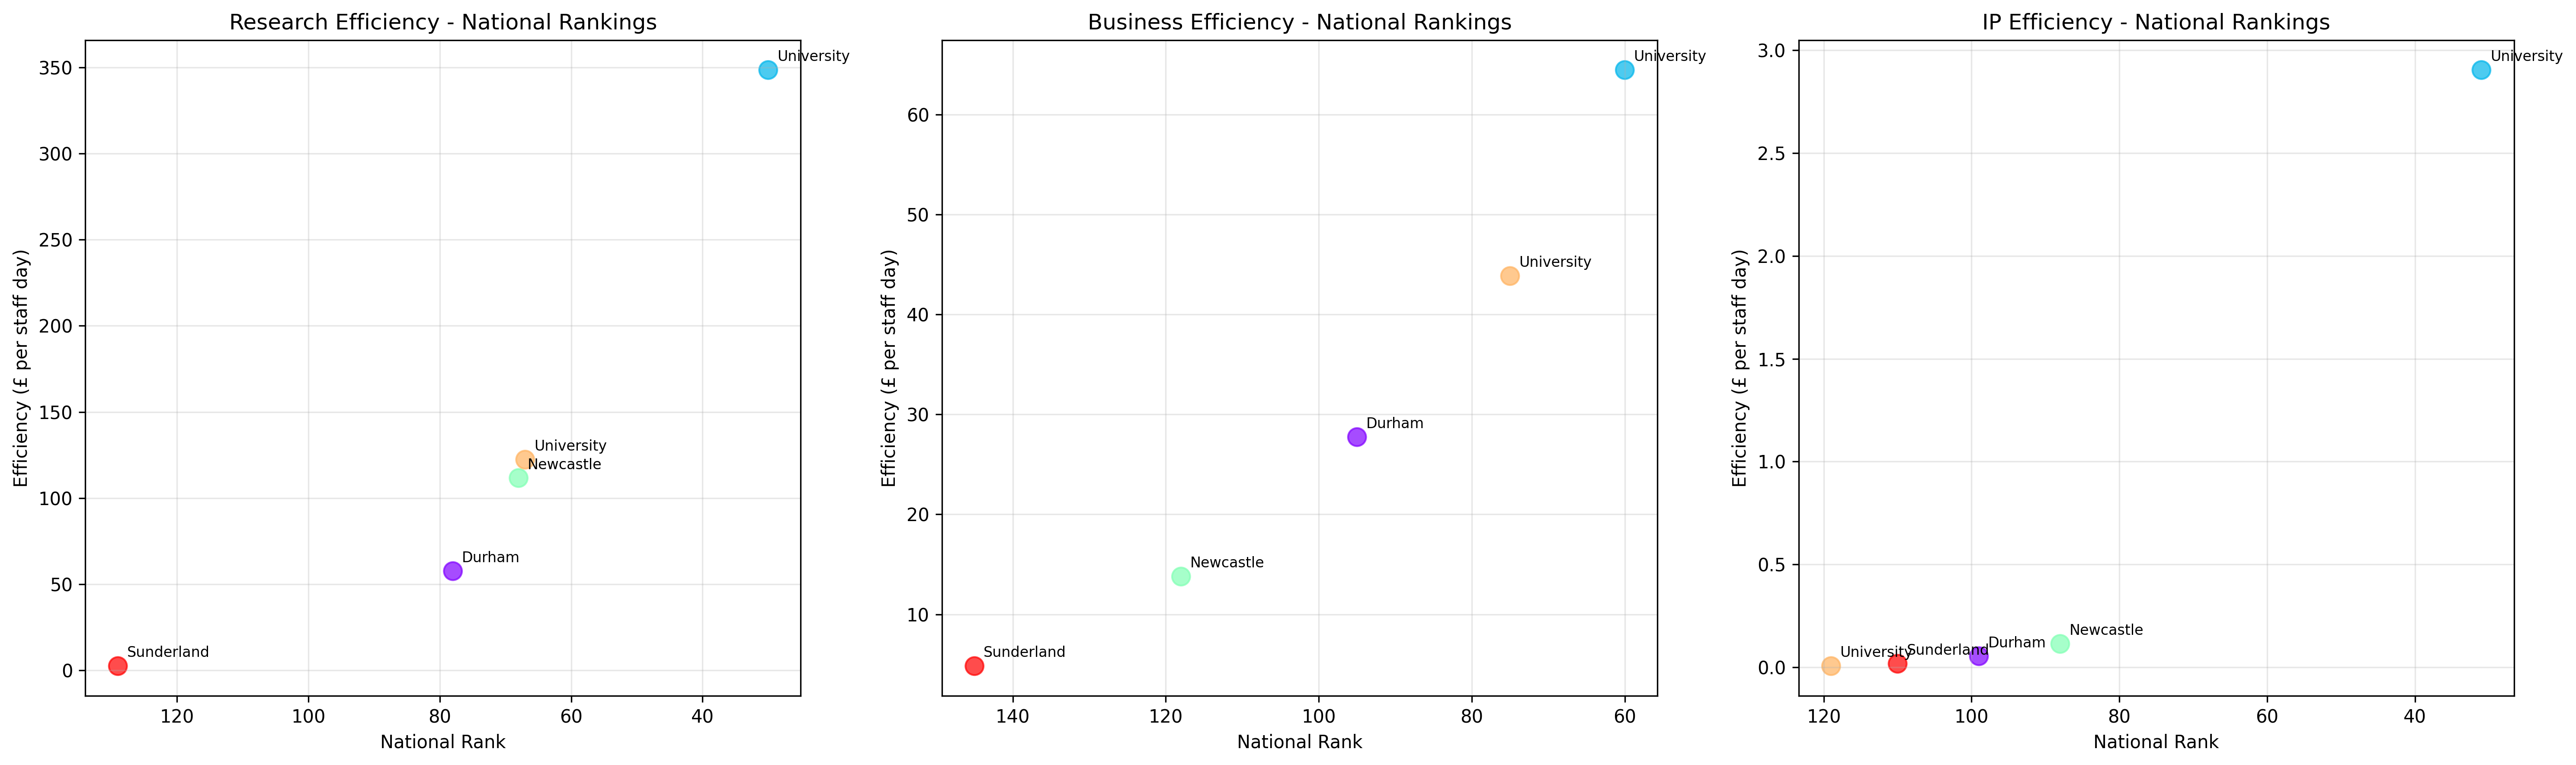
\includegraphics[width=0.99\textwidth]{Fig/figure40.national_efficiency_rankings.png}
\caption{National Efficiency Rankings}
\label{fig:national-efficiency-rankings}
\end{figure}

These trends suggest that efficiency gains in research and business services are possible with targeted efforts, while IP monetization remains an underutilized opportunity across the region. Figure~\ref{fig:efficiency-trends} demonstrates the temporal evolution of efficiency metrics, showing Durham's gradual improvement in recent years.

\subsubsection{National Ranking Performance}

\begin{itemize}
    \item \textbf{Research:} Newcastle ranks 29th nationally, placing it among the top 15\%. Teesside (64th) and Northumbria (69th) perform above average. Durham ranks 78th, below both despite its research intensity. Sunderland ranks near the bottom at 131st.
    
    \item \textbf{Business:} Newcastle ranks 60th, while Teesside achieves 75th. Durham's position at 95th signals room for improved business-facing efficiency. Sunderland ranks 145th, indicating minimal output per staff day in this area.
    
    \item \textbf{IP:} Only Newcastle achieves a strong IP efficiency ranking (35th). Others fall below the 85th percentile, with Durham at 71st and Sunderland and Teesside near 110-120.
    
    \item \textbf{CPD:} Teesside leads regionally with a national ranking of 39th, followed by Northumbria (64th) and Sunderland (133rd). Newcastle (140th) and Durham (162nd) rank in the bottom third nationally, highlighting significant opportunities for CPD efficiency improvement.
\end{itemize}

The rankings confirm that while Newcastle is a national leader in staff-driven income generation, Durham's per-capita returns place it at a mid-tier level. This discrepancy between scale and efficiency presents an actionable area for improvement. As shown in Figure~\ref{fig:ranking-changes}, Durham's performance trajectory demonstrates consistent regional positioning despite efficiency challenges. As shown in Figure~\ref{fig:ranking-changes}, Durham's performance trajectory demonstrates consistent regional positioning despite efficiency challenges.

\subsubsection{Performance Efficiency Summary}

Durham University maintains strong total outputs but underperforms relative to peers when normalized by academic staff time. While Newcastle University excels in research and IP efficiency, Teesside University leads in CPD efficiency, and other institutions show domain-specific strengths. IP efficiency remains universally low, while CPD efficiency shows significant regional variation, pointing to structural barriers in translating innovation into revenue and opportunities for professional development monetization. The performance efficiency analysis, using output-to-input ratios across income streams, highlights notable differences among North East institutions. Durham University ranks fourth in research efficiency within the region, with moderate performance in business services and IP income conversion. This suggests room for improvement in translating resources into measurable outcomes. Nationally, Durham places in the mid-tier range, indicating potential for operational enhancement. However, the analysis also reveals underperformance in CPD and business income efficiency compared to national benchmarks. While the university performs well in securing research grants, its ability to monetize business services and lifelong learning lags behind leading institutions. These insights point to a need for rebalancing investment-to-return structures across income categories.

\textbf{Strategic Implications:}
\begin{itemize}
    \item \textbf{For Durham:} Improve resource alignment and staff deployment strategies to raise unit productivity, particularly in IP commercialization, business consultancy, and CPD monetization. Learn from Teesside's CPD efficiency model to enhance professional development revenue generation.
    
    \item \textbf{For Policy Makers:} Support capacity-building for lower-efficiency institutions (e.g., Sunderland), and promote regional knowledge exchange models that reward efficient delivery as well as scale.
\end{itemize}

\subsection{Resilience and Risk Analysis}
\label{sec:resilience-risk}

This section investigates the financial resilience and risk exposure of North East universities by analyzing income volatility and concentration across four key domains: research, business services, continuing professional development (CPD), and intellectual property (IP), as pioneered by Markowitz (1952) \cite{markowitz1952portfolio} and Sharpe (1964) \cite{sharpe1964capital}. Resilience is interpreted as an institution's ability to maintain stable income streams and avoid overreliance on a small number of sources.

\subsubsection{Methodology Overview}

Two primary methods are used in this analysis:

1. \textbf{Income Volatility} is assessed using the coefficient of variation (CV), calculated as, $\mathrm{CV}=\frac{\text{Standard Deviation}}{\text{Mean Income}}$. Lower CV indicates greater income stability over the 10-year period.

2. \textbf{Income Concentration} is measured using the Herfindahl-Hirschman Index (HHI) and Maximum Source Share, based on the proportional contributions of different income sources. Higher HHI indicates greater income dependency and lower diversification.

\subsubsection{Volatility Comparison - North East Universities}

\begin{figure}[h]
\centering
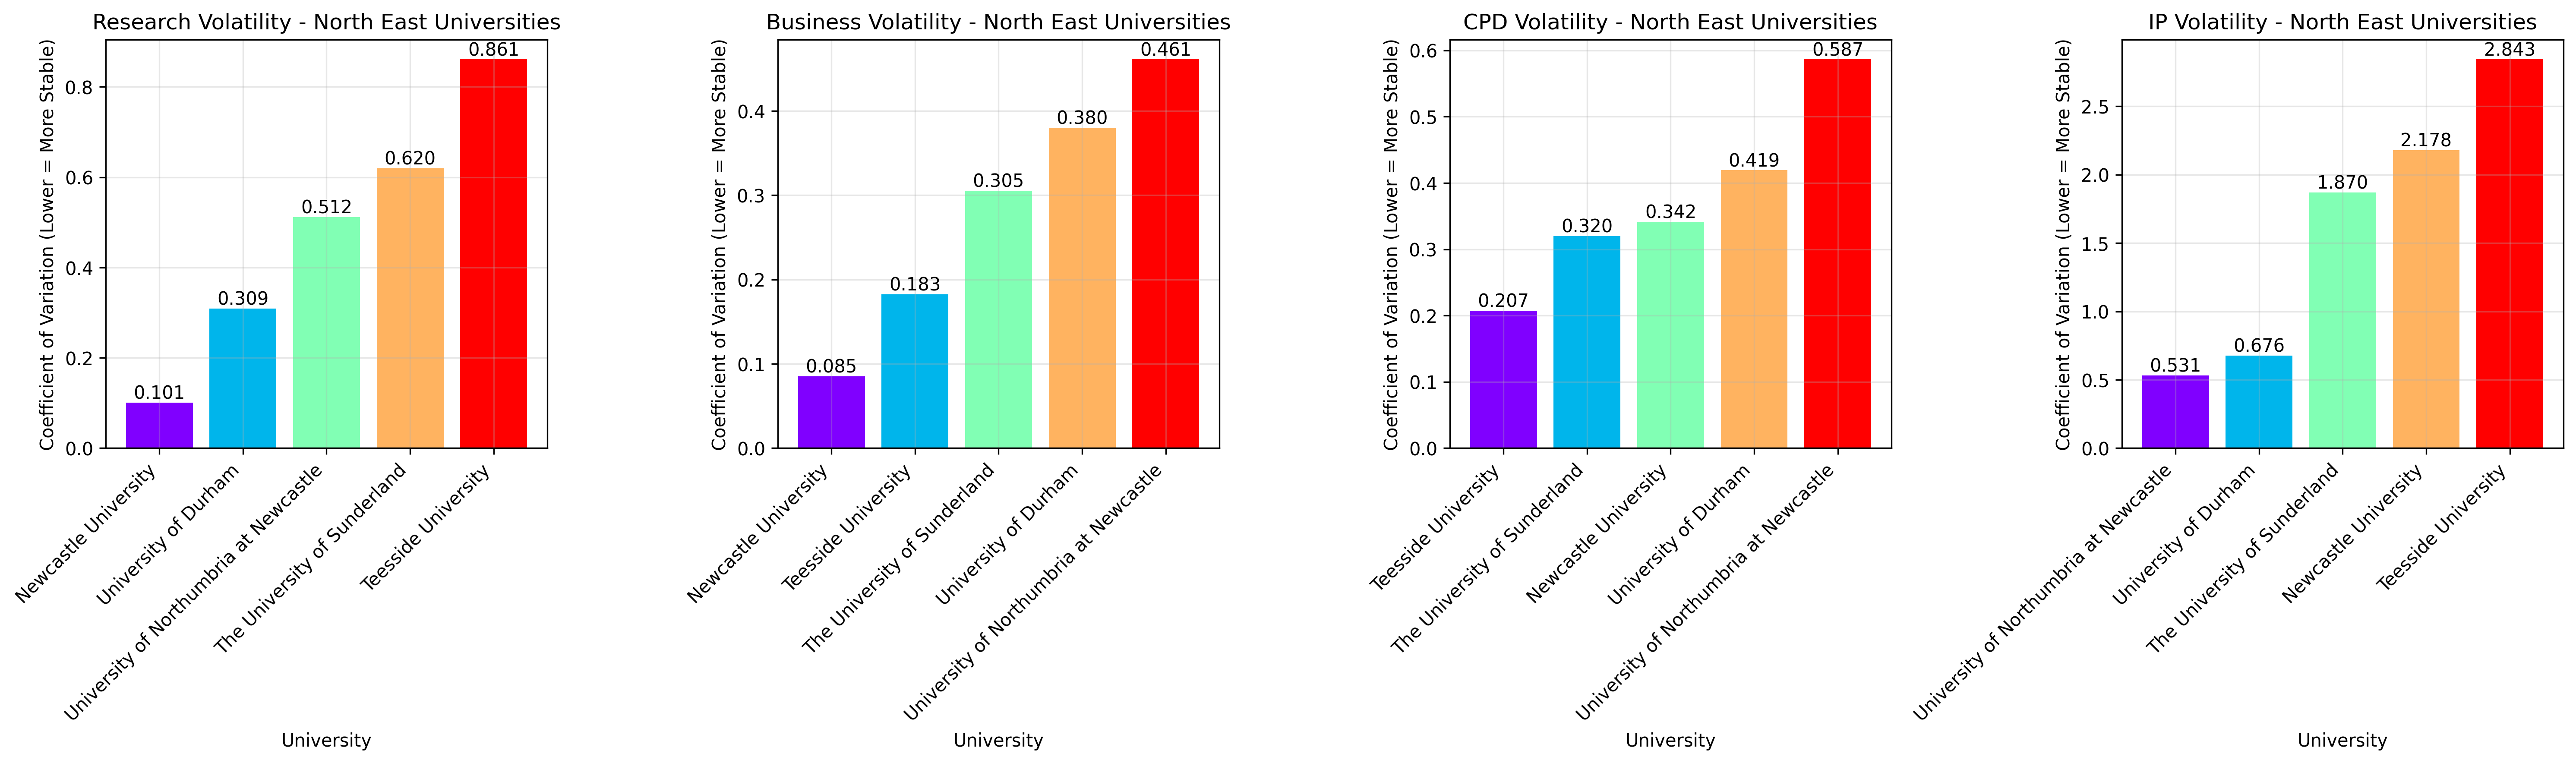
\includegraphics[width=0.99\textwidth]{Fig/figure41.ne_volatility_comparison.png}
\caption{Income Volatility by Domain}
\label{fig:ne-volatility-comparison}
\end{figure}

\begin{figure}[h]
\centering
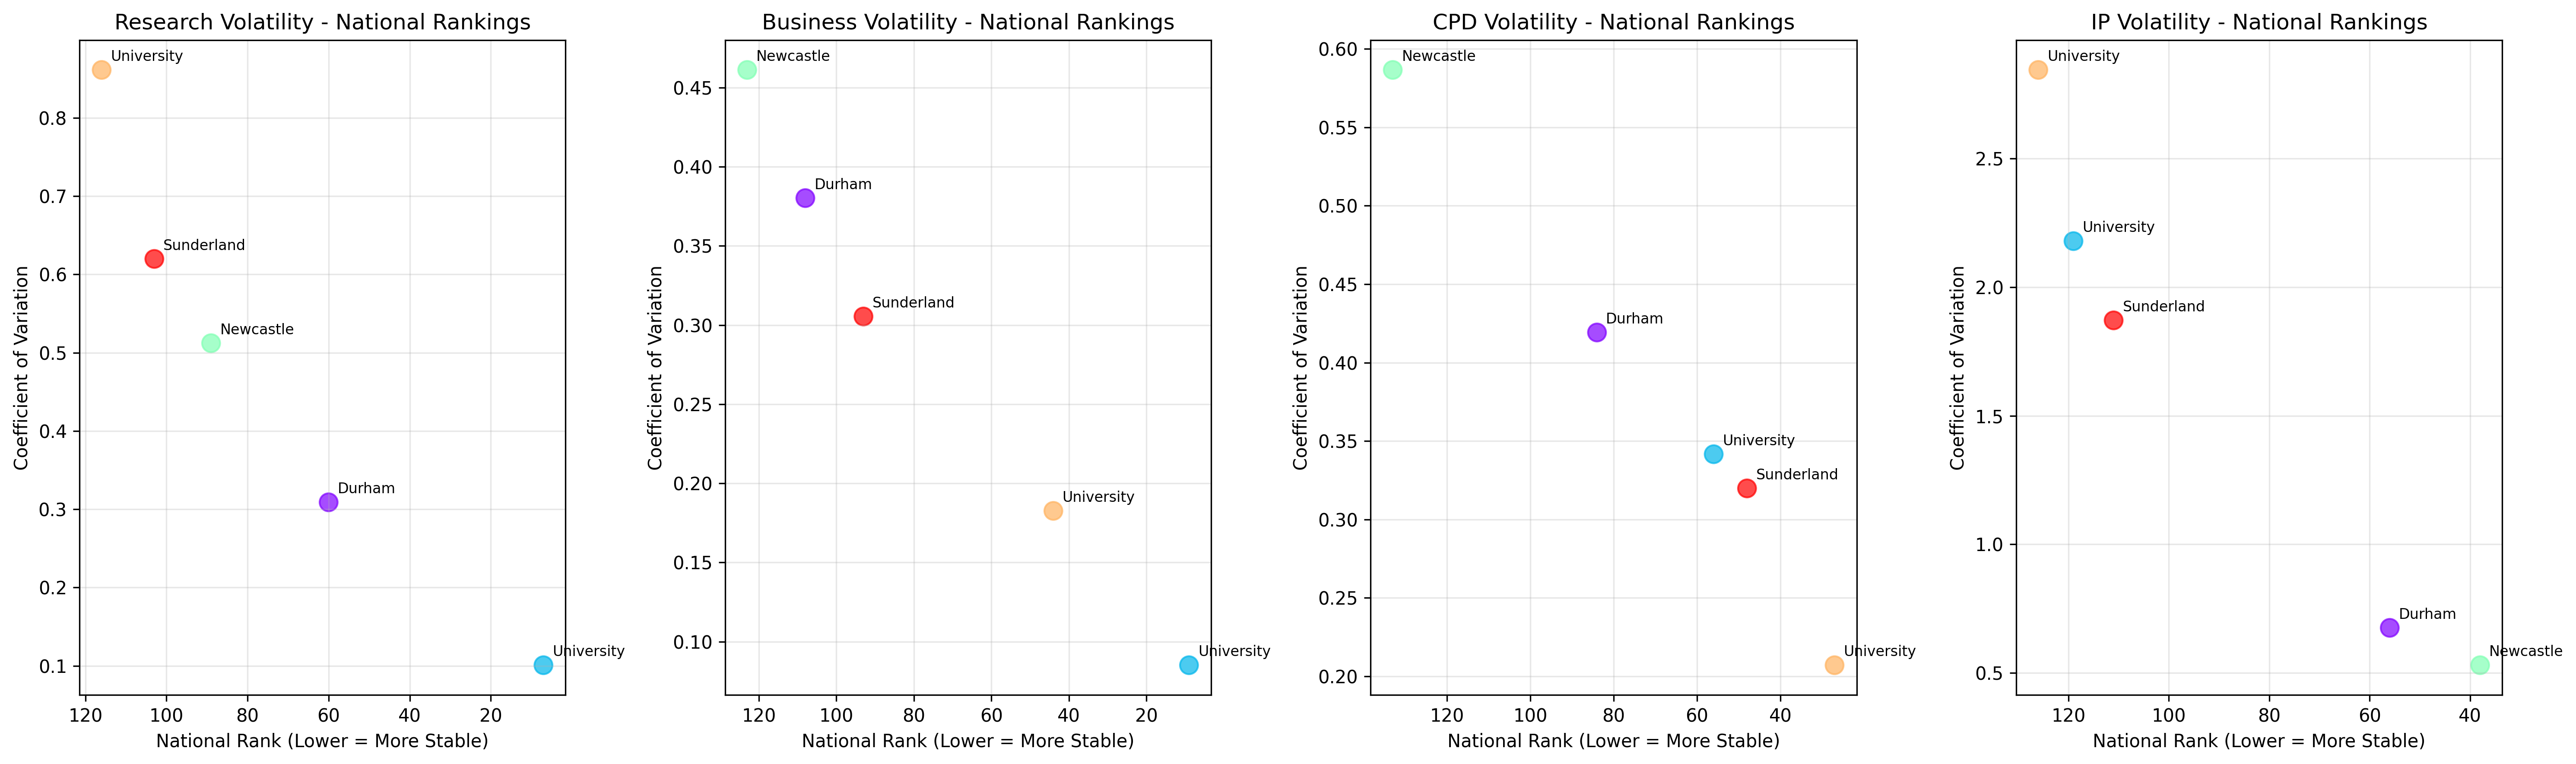
\includegraphics[width=0.99\textwidth]{Fig/figure42.national_volatility_rankings.png}
\caption{National Volatility Rankings}
\label{fig:national-volatility-rankings}
\end{figure}

\begin{itemize}
    \item \textbf{Research:} Newcastle University exhibits the highest stability ($\mathrm{CV}=0.125$), significantly outperforming all peers. Durham shows moderate stability ($\mathrm{CV}=0.324$), while Northumbria ($\mathrm{CV}=0.500$) and Sunderland ($\mathrm{CV}=0.761$) show higher volatility. Teesside shows the highest volatility ($\mathrm{CV}=0.937$), indicating irregular research income patterns.
    
    \item \textbf{Business Services:} Again, Newcastle leads with $\mathrm{CV}=0.085$, followed by Teesside ($\mathrm{CV}=0.183$) and Sunderland ($\mathrm{CV}=0.305$). Durham shows moderate instability ($\mathrm{CV}=0.380$), while Northumbria ranks lowest with $\mathrm{CV}=0.461$.
    
    \item \textbf{CPD:} Northumbria ranks best ($\mathrm{CV}=0.114$), followed by Teesside ($\mathrm{CV}=0.215$) and Sunderland ($\mathrm{CV}=0.270$). Newcastle shows moderate variation ($\mathrm{CV}=0.290$), while Durham displays higher variation ($\mathrm{CV}=0.340$).
    
    \item \textbf{IP:} All universities show high volatility in IP income. Northumbria ($\mathrm{CV}=0.531$) and Sunderland ($\mathrm{CV}=1.870$) are relatively more stable than Durham ($\mathrm{CV}=2.408$), Newcastle ($\mathrm{CV}=2.150$), and Teesside ($\mathrm{CV}=2.843$), reflecting erratic licensing revenue patterns.
\end{itemize}

\subsubsection{National Volatility Rankings}

\begin{itemize}
    \item \textbf{Research:} Newcastle ranks 7th nationally (among 228 institutions), while Durham sits at 58th, reflecting above-average resilience. Teesside (114th) and Sunderland (105th) fall beyond the 100th rank.
    
    \item \textbf{Business:} Newcastle (9th) and Teesside (44th) perform well; Sunderland ranks 93rd, Durham ranks 108th, and Northumbria ranks 123rd, indicating above-average fluctuation.
    
    \item \textbf{CPD:} Northumbria (10th) and Teesside (36th) show excellent performance. Sunderland (57th) and Newcastle (67th) perform well, while Durham ranks 84th, signaling medium resilience.
    
    \item \textbf{IP:} National volatility in IP is high. Northumbria (26th) shows relatively good performance, while Sunderland (109th), Newcastle (115th), Durham (121st), and Teesside (125th) fall into the high-risk range.
\end{itemize}

The national perspective confirms Newcastle's strong position as one of the most resilient institutions in the UK, while Durham maintains mid-tier stability. Teesside and Sunderland face higher volatility, particularly in IP and research domains.

\subsubsection{Income Trend Analysis}

The following summary presents trend statistics across academic years, including year-on-year changes, peak gains and losses, and volatility (as standard deviation of \% changes). Table~\ref{tab:income-trends} provides detailed trend analysis data for all income streams across North East universities.

\begin{table}[h]
\centering
\caption{Income Trends Analysis - North East Universities (2014/15-2023/24)}
\vspace{0.1cm}
\resizebox{0.95\textwidth}{!}{%
\begin{tabular}{|l|l|l|l|l|l|l|l|}
\hline \textbf{University} & \textbf{Income Type} & \textbf{Total (\textsterling)} & \textbf{Avg (\textsterling)} & \textbf{Min (\textsterling)} & \textbf{Max (\textsterling)} & \textbf{Avg Change (\%)} & \textbf{Volatility (\%)} \\
\hline \multirow{4}{*}{University of Durham} & Research & 216,850 & 24,094 & 10,776 & 34,966 & 18.5 & 34.6 \\
\cline{2-8} & Business & 418,390 & 41,839 & 22,422 & 69,630 & -2.7 & 25.5 \\
\cline{2-8} & CPD & 8,357 & 836 & 422 & 1,225 & 25.3 & 69.9 \\
\cline{2-8} & IP & 6,687 & 669 & 23 & 5,201 & 136.4 & 246.2 \\
\hline \multirow{4}{*}{Newcastle University} & Research & 1,105,304 & 122,812 & 107,246 & 149,154 & 4.0 & 16.1 \\
\cline{2-8} & Business & 726,188 & 72,619 & 61,312 & 79,546 & 0.6 & 8.3 \\
\cline{2-8} & CPD & 24,849 & 2,485 & 1,517 & 3,950 & 15.9 & 54.5 \\
\cline{2-8} & IP & 36,868 & 3,687 & 557 & 26,223 & 163.7 & 462.4 \\
\hline \multirow{4}{*}{University of Northumbria at Newcastle} & Research & 134,470 & 14,941 & 5,776 & 23,980 & 20.8 & 19.1 \\
\cline{2-8} & Business & 59,166 & 5,917 & 3,996 & 13,414 & 13.2 & 53.3 \\
\cline{2-8} & CPD & 74,062 & 7,406 & 5,852 & 8,344 & -0.4 & 9.5 \\
\cline{2-8} & IP & 527 & 53 & 3 & 88 & 159.7 & 481.4 \\
\hline \multirow{4}{*}{Teesside University} & Research & 68,844 & 7,649 & 3,214 & 24,662 & 32.3 & 39.5 \\
\cline{2-8} & Business & 114,326 & 11,433 & 8,892 & 15,050 & -1.0 & 14.0 \\
\cline{2-8} & CPD & 71,538 & 7,154 & 5,232 & 10,026 & 4.5 & 15.2 \\
\cline{2-8} & IP & 21 & 2 & 0 & 19 & -100.0 & 0.0 \\
\hline \multirow{4}{*}{The University of Sunderland} & Research & 2,744 & 305 & 0 & 762 & 9.6 & 133.0 \\
\cline{2-8} & Business & 21,088 & 2,109 & 974 & 3,290 & 19.2 & 38.5 \\
\cline{2-8} & CPD & 14,229 & 1,423 & 954 & 2,128 & 8.8 & 37.5 \\
\cline{2-8} & IP & 155 & 16 & 0 & 83 & -63.1 & 54.9 \\
\hline
\end{tabular}
}
\label{tab:income-trends}
\end{table}

As shown in Table~\ref{tab:income-trends}, Durham University demonstrates significant volatility across all income streams, with particularly high volatility in business services (25.5\%) and research income (34.6\%). The university shows moderate average growth rates in IP income (136.4\%) but negative growth in business services (-2.7\%), accompanied by year-to-year fluctuations. Newcastle University shows more stable patterns, particularly in research income with lower volatility (16.1\%) and moderate average growth (4.0\%). Teesside University demonstrates the most stable CPD income with low volatility (15.2\%) and consistent growth (4.5\%), while Northumbria shows exceptional stability in CPD with minimal volatility (9.5\%).

\begin{itemize}
    \item \textbf{Research Trends:} Newcastle and Durham show large standard deviations in annual growth, primarily due to pandemic-related dips and post-COVID rebounds. Sunderland's low average income and frequent drops produce erratic volatility patterns. Deep analysis reveals that Durham's research income volatility ($\mathrm{CV}=0.324$) is primarily driven by two structural factors: (1) the concentration of funding in BEIS Research Councils (60.7\% of total), which creates dependency on government policy cycles, and (2) the irregular timing of large collaborative projects, leading to significant year-on-year fluctuations in peak years. This pattern suggests that Durham's research strategy, while successful in securing major grants, may benefit from more diversified funding sources to reduce volatility.
    
    \item \textbf{Business Trends:} All institutions show significant year-on-year fluctuation, with frequent declines and spikes, suggesting high sensitivity to partnership cycles and external funding schemes. Durham and Newcastle exhibit negative trend slopes, while Teesside maintains modest positive growth. Further investigation reveals that Durham's business services volatility ($\mathrm{CV}=0.380$) stems from three key factors: (1) the dominance of contract research (64.1\% of business income) which is highly sensitive to external funding cycles, (2) the concentration of clients in non-commercial organizations (30.1\% of contracts), making the institution vulnerable to public sector budget cuts, and (3) the limited engagement with SMEs (3.1\% of contracts), missing opportunities for more stable, diversified income streams. This analysis suggests that Durham could enhance business income stability by expanding SME partnerships and diversifying service offerings beyond traditional contract research.
    
    \item \textbf{CPD Trends:} Teesside and Northumbria show strong long-term upward trends. Durham's CPD income trend is slightly negative despite modest average annual growth, suggesting inconsistent returns. Detailed analysis uncovers the root cause of Durham's CPD underperformance: despite delivering 98,190 learner days (ranking 4th regionally), the revenue generation efficiency is extremely low at \textsterling 0.085 per learner day, compared to Teesside's \textsterling 0.211 efficiency. This inefficiency stems from (1) the high proportion of free or subsidized courses (83.1\% of total value), (2) the focus on non-commercial organizations (52.8\% of courses) which typically pay lower rates, and (3) the lack of premium CPD offerings that could command higher fees. The analysis suggests that Durham could significantly improve CPD profitability by developing specialized, high-value professional development programs while maintaining its commitment to public engagement.
    
    \item \textbf{IP Trends:} All institutions display extreme volatility and irregular growth. Year-on-year changes often exceed ±100\%, with frequent income collapses (e.g., 100\% decrease). Trend analysis is inconclusive for most due to unstable series. In-depth examination reveals that Durham's IP volatility ($\mathrm{CV}=2.408$) is fundamentally different from other institutions: while Newcastle's high volatility ($\mathrm{CV}=2.150$) stems from large, irregular licensing deals, Durham's volatility reflects a systematic commercialization challenge. Specifically, (1) only 1.7\% of licenses generate income (30 out of 1,719 total licenses), indicating a fundamental disconnect between IP creation and commercialization success, (2) the average income per license (\textsterling 10.66) is significantly below the national average (\textsterling 19.30), suggesting undervaluation of IP assets, and (3) the concentration in non-software licenses (85.8\% of portfolio) in a market increasingly favoring software and digital IP. This analysis indicates that Durham's IP strategy requires fundamental restructuring, focusing on commercialization pipeline development rather than portfolio expansion.
\end{itemize}

The trend analysis reinforces volatility findings. CPD appears to offer the most stable and predictable income opportunities, while IP continues to pose the greatest financial uncertainty. This comprehensive volatility analysis reveals a critical insight: Durham's financial resilience is not uniformly distributed across income streams, but rather follows a distinct pattern where stability correlates with institutional control over pricing and client relationships. Research income, while volatile, benefits from government funding stability; CPD offers predictable returns but suffers from pricing inefficiency; business services show moderate volatility due to external dependency; and IP income exhibits extreme volatility due to commercialization pipeline failures. This pattern suggests that Durham's financial strategy should prioritize (1) developing premium CPD offerings to capture higher margins, (2) expanding SME partnerships to reduce business service volatility, and (3) restructuring IP commercialization processes to improve income predictability, rather than simply expanding existing activities.

\subsubsection{Income Concentration and Diversification}

An analysis of income sources across the five domains reveals significant differences in diversification. Table~\ref{tab:income-concentration} presents the Herfindahl-Hirschman Index (HHI) values and income concentration metrics for North East universities.

\begin{table}[h]
\centering
\caption{Income Concentration Analysis - North East Universities}
\vspace{0.1cm}
\resizebox{0.8\textwidth}{!}{%
\begin{tabular}{|l|l|l|l|l|}
\hline \textbf{University} & \textbf{Total Income (\textsterling)} & \textbf{HHI Index} & \textbf{Max Source Share (\%)} & \textbf{Income Sources} \\
\hline University of Durham & \textsterling 663,556 & 0.211 & 31.4\% & 12 \\
\hline Newcastle University & \textsterling 1,905,179 & 0.195 & 29.3\% & 12 \\
\hline University of Northumbria at Newcastle & \textsterling 272,053 & 0.181 & 27.2\% & 12 \\
\hline Teesside University & \textsterling 277,953 & 0.161 & 25.7\% & 12 \\
\hline The University of Sunderland & \textsterling 72,188 & 0.309 & 47.1\% & 8 \\
\hline
\end{tabular}
}
\label{tab:income-concentration}
\end{table}

As shown in Table~\ref{tab:income-concentration}, Durham University demonstrates a moderately diversified income structure, with a total income concentration HHI\footnote{Total income concentration HHI measures the diversification of all income sources across the five main domains (research, business services, IP, CPD, and regeneration), where lower values indicate better diversification across income streams.} value of 0.211 and a maximum source share of 31.4\%, indicating no overwhelming reliance on any single funder or activity. Newcastle University shows the best diversification with the lowest HHI (0.195) and maximum source share (29.3\%), despite having the highest total income. Teesside and Northumbria show good diversification with HHI values below 0.20. In contrast, Sunderland exhibits the highest concentration (HHI = 0.309) with a maximum source share of 47.1\%, indicating limited diversification due to small-scale activity and dependency on single-stream income sources.

Institutions with higher volatility often show greater income concentration, suggesting that improved diversification could enhance financial resilience. Durham should focus on diversifying income sources to reduce concentration risk and improve financial stability.

\subsubsection{Resilience and Risk Summary}

Durham University demonstrates moderate financial stability across most domains. In research income, Durham shows a coefficient of variation (CV) of 0.324, indicating moderate volatility compared to regional peers, with Newcastle showing exceptional consistency (CV = 0.125). Table~\ref{tab:research-volatility} summarizes CV values, along with the mean and standard deviation of research income across the five universities.
\vspace{0.25cm}
\begin{table}[h]
\centering
\caption{Research Income Volatility Analysis - North East Universities}
\vspace{0.1cm}
\resizebox{0.7\textwidth}{!}{%
\begin{tabular}{|l|l|l|l|}
\hline \textbf{University} & \textbf{Coefficient of Variation} & \textbf{Mean Income (\textsterling )} & \textbf{Std Dev (\textsterling )} \\
\hline Newcastle University & 0.125 & \textsterling 122,812 & \textsterling 15,297 \\
\hline University of Durham & 0.324 & \textsterling 24,094 & \textsterling 7,798 \\
\hline University of Northumbria at Newcastle & 0.500 & \textsterling 14,941 & \textsterling 7,470 \\
\hline The University of Sunderland & 0.761 & \textsterling 305 & \textsterling 232 \\
\hline Teesside University & 0.937 & \textsterling 7,649 & \textsterling 7,167 \\
\hline
\end{tabular}
}
\label{tab:research-volatility}
\end{table}

As seen in Table~\ref{tab:research-volatility} and Figure~\ref{fig:ne-volatility-comparison}, Newcastle enjoys both high income levels and low volatility, while Durham maintains stability despite its moderate income. Teesside and Sunderland show significant instability, suggesting higher exposure to financial risk.

From a national perspective (Figure 42), Durham ranks within the top third of UK institutions for research resilience and performs moderately in business and CPD domains. However, its IP income remains highly volatile ($\mathrm{CV}=2.408$) and ranks 121st nationally, reflecting exposure to commercial licensing risk.

Durham's income diversification profile is relatively strong, with no single income stream accounting for more than 50\% and a Herfindahl-Hirschman Index (HHI) value under 0.35. This distribution mitigates systemic risk and reinforces the institution's medium resilience tier.

\subsubsection{Resilience Risk Analysis Summary}
The resilience risk analysis evaluates volatility in income streams as a proxy for institutional stability. Durham shows medium risk exposure nationally, with relatively stable trends in research income and IP income. However, significant year-over-year variability is observed in business services and spinout performance. Compared to Newcastle and Teesside, Durham demonstrates moderate resilience, with volatility scores near the national median.

At the regional level, Northumbria emerges as highly volatile, whereas Newcastle maintains greater stability. Durham's resilience profile suggests robustness in core academic outputs, but it also signals exposure in commercialization and entrepreneurial metrics. Improving stability in these areas is essential to weather sector-wide funding fluctuations and policy shifts.

\subsection{Trend Prediction Analysis}
\label{sec:trend-prediction}

To enhance the robustness and interpretability of forecasting, I expand beyond traditional trend models to incorporate advanced time series and machine learning techniques, as established by Box et al. (2015) \cite{box2015time} and Hamilton (1994) \cite{hamilton1994time}:

\begin{itemize}
    \item \textbf{Linear Regression:} A simple deterministic model capturing overall direction.
    \item \textbf{Exponential Smoothing:} A statistical method that gives more weight to recent data, useful for short-term trends, as developed by Hyndman and Athanasopoulos (2018) \cite{hyndman2018forecasting}.
    \item \textbf{Random Forest:} An ensemble learning model capturing non-linear interactions and uncertainty, as introduced by Breiman (2001) \cite{breiman2001random}.
    \item \textbf{ARIMA (AutoRegressive Integrated Moving Average):} A classic time series model adept at modeling autocorrelations and structural changes, as developed by Box et al. (2015) \cite{box2015time}.
    \item \textbf{XGBoost (Extreme Gradient Boosting):} A powerful non-linear tree-based model capable of modeling complex dependencies and outliers, as created by Chen and Guestrin (2016) \cite{chen2016xgboost}.
    \item \textbf{Clustering (K-Means \& Hierarchical):} Enables unsupervised grouping of universities based on trend evolution, identifying similarity patterns, as introduced by MacQueen (1967) \cite{macqueen1967methods} and Ward (1963) \cite{ward1963hierarchical}.
\end{itemize}

These five predictive methods and two clustering strategies offer a comprehensive understanding of trend trajectories and institutional positioning. Here I choose one of the methods as an example, for other results please refer to the GitHub repository. Additional forecasting results for all models are presented in Figures~\ref{fig:trend-predictions-linear-regression}, \ref{fig:trend-predictions-random-forest}, \ref{fig:trend-predictions-arima}, and \ref{fig:trend-predictions-xgboost} in the Appendix, along with comprehensive trend data in Table~\ref{tab:forecasted-trends}. The methodological diversity addresses a critical limitation of single-model approaches: while linear regression captures long-term trends, it misses cyclical patterns that exponential smoothing reveals; random forest handles non-linear relationships but may overfit to recent data; ARIMA models temporal dependencies but struggles with structural breaks; and XGBoost captures complex interactions but requires careful hyperparameter tuning. The clustering analysis provides additional validation by identifying whether Durham's predicted trajectory aligns with similar institutions or represents a unique path. \textbf{This multi-model ensemble approach reduces prediction uncertainty and provides confidence intervals for strategic planning, addressing the fundamental challenge of forecasting in highly volatile, policy-sensitive environments.}


\begin{figure}[h]
\centering
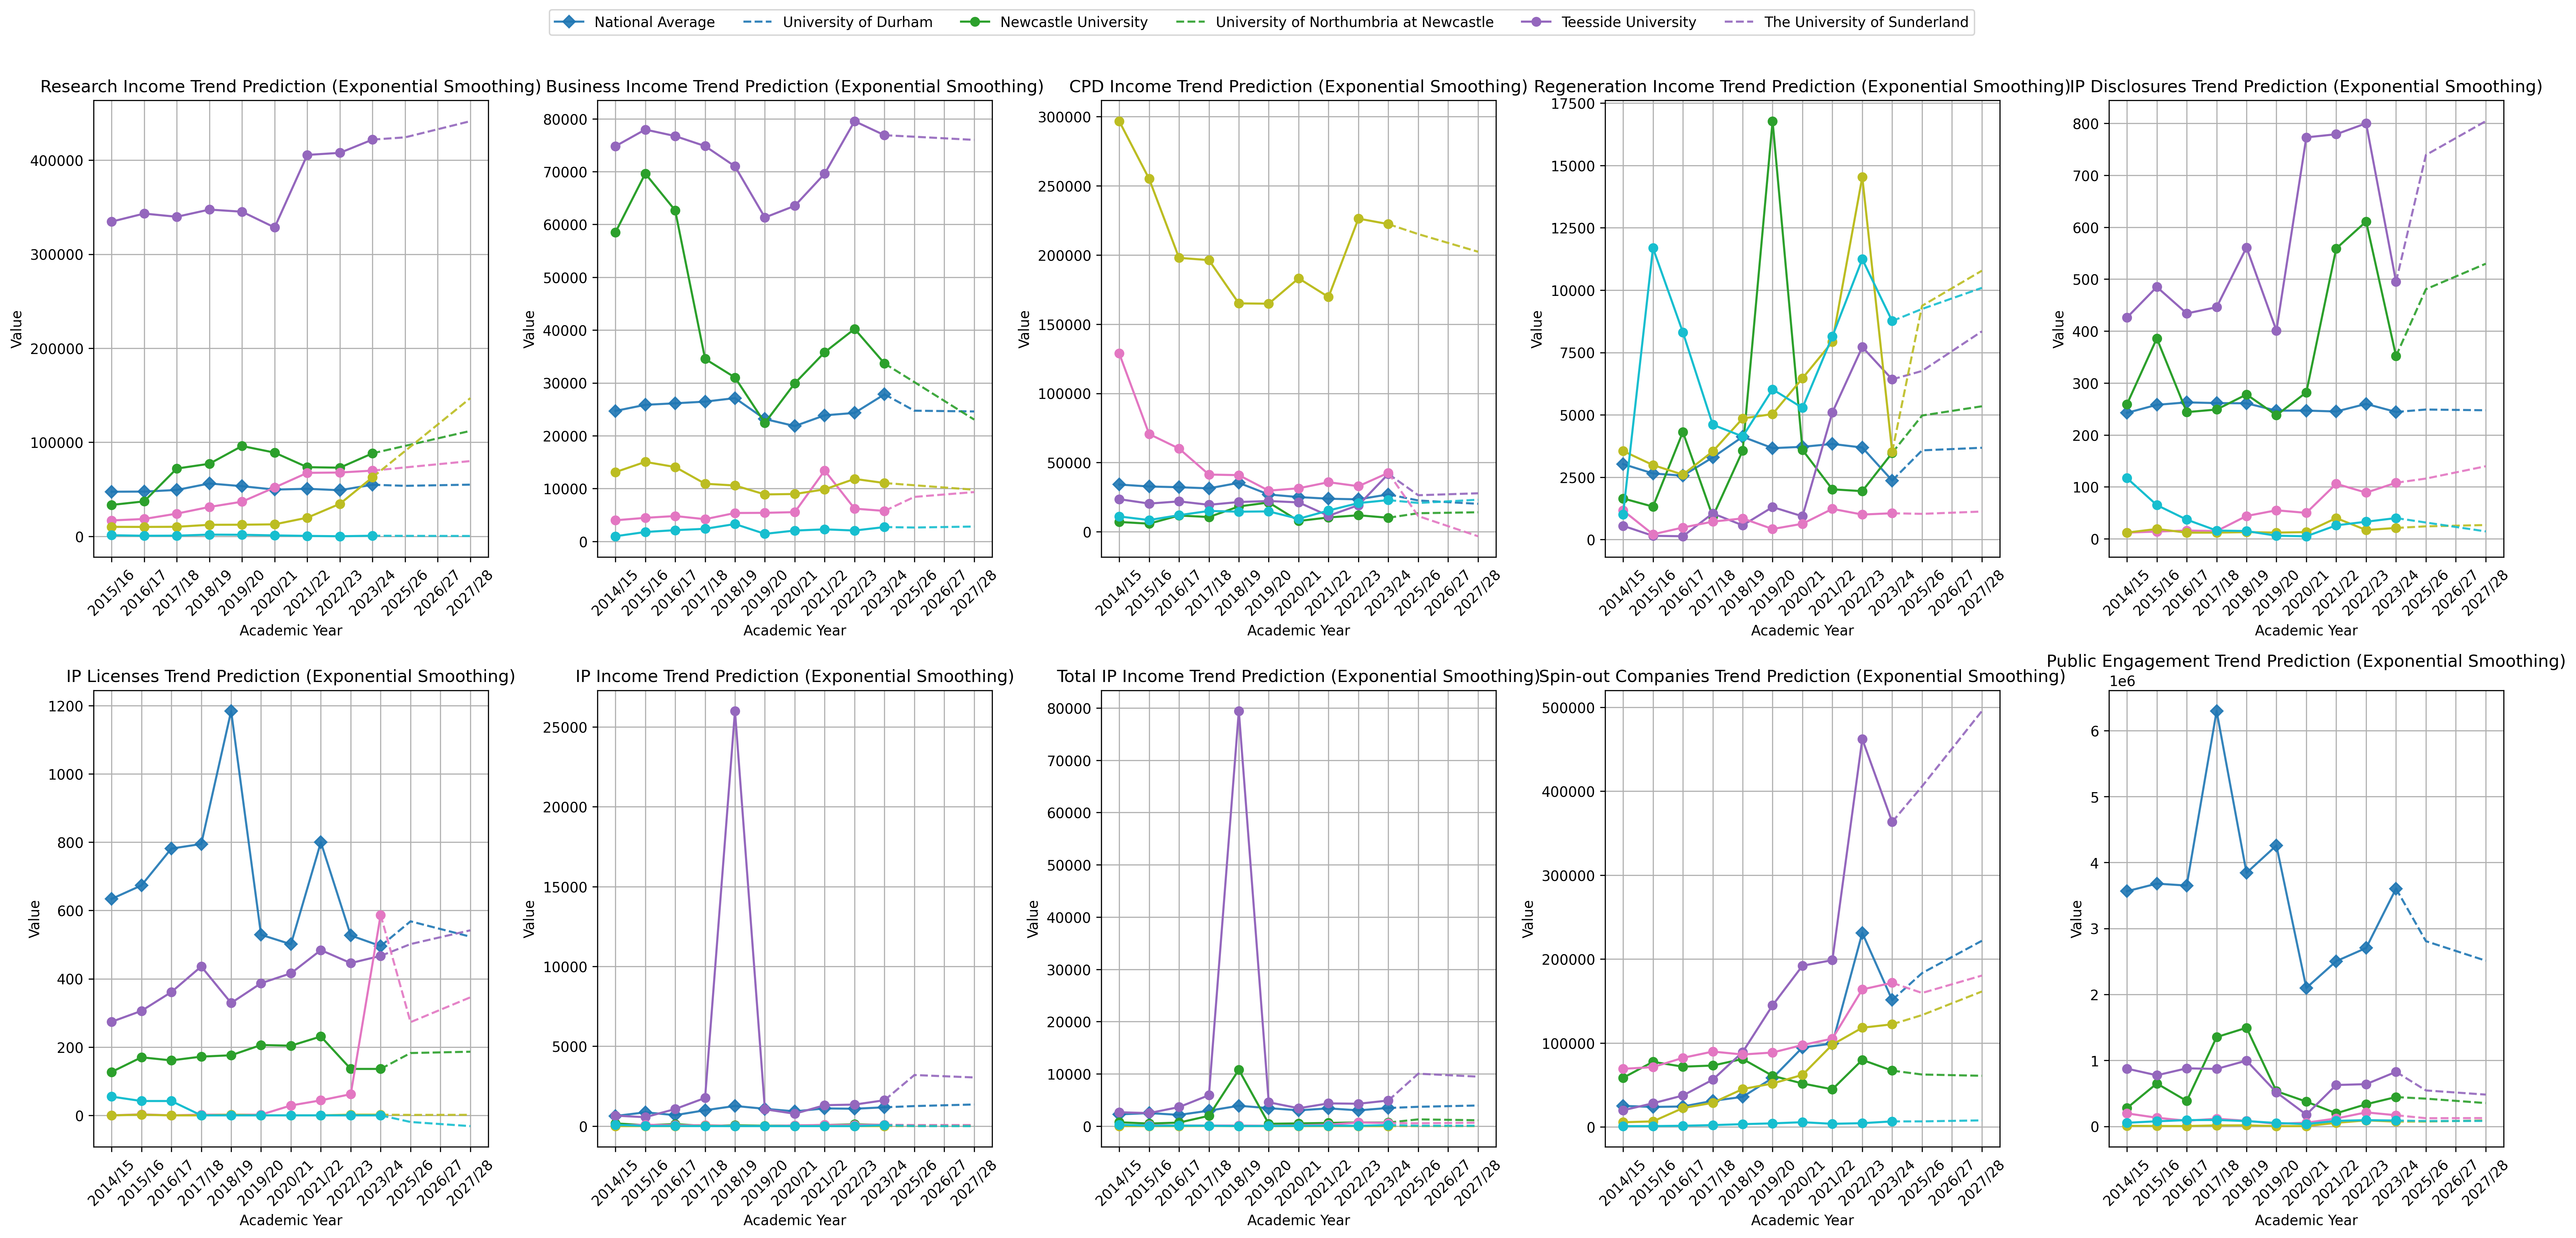
\includegraphics[width=0.99\textwidth]{Fig/figure43.trend_predictions_exponential_smoothing.png}
\caption{Trend predictions exponential smoothing}
\label{fig:trend-predictions-exponential-smoothing}
\end{figure}

\subsubsection{Income Trend Analysis}

\begin{itemize}
    \item \textbf{Research Income Trends:} Forecasting results for Durham University's research income show strong potential growth. Linear regression predicts a +18.82\% increase, while exponential smoothing estimates a +26.19\% rise. However, the random forest model suggests a possible -7.85\% decline, introducing a degree of caution. Compared to the national average, which ranges from -2.33\% to -1.75\%, Durham's predictions are notably more optimistic under deterministic models.
    
    \item \textbf{Business Income Trends:} Projections for business income are highly volatile. Linear regression forecasts a significant -54.84\% decline, and exponential smoothing indicates a -31.56\% drop. In contrast, the random forest model projects a modest +6.77\% increase. Nationally, business income trends consistently point downward, with an average decline of -11.64\%, suggesting structural challenges in this area across the sector.
    
    \item \textbf{CPD Income Trends:} Durham's CPD income outlook shows mixed signals. Linear regression and exponential smoothing predict declines (-15.62\% and -15.15\%, respectively), while random forest suggests a similar decline (-11.13\%). This contrasts with the national average, which indicates a substantial -26.54\% decline. Despite the projected decline, Durham's performance remains better than the national average, suggesting relative resilience in CPD activities.
\end{itemize}

The income trend analysis presents a mixed but insightful outlook. Research income shows strong growth potential despite minor risk flagged by the random forest model. Business services exhibit high volatility and sector-wide decline, calling for stabilization efforts. CPD income trends show projected declines but remain more resilient than national benchmarks, suggesting relative stability in this area.

\subsubsection{IP Performance Trends}

\begin{itemize}
    \item \textbf{IP Disclosures Trends:} Durham's IP disclosures are projected to grow significantly, with both linear regression and exponential smoothing models forecasting +50.49\% growth, and the random forest model predicting +28.84\%. These figures stand in stark contrast to the national average growth of just +1.34\%, highlighting Durham's strength in IP generation and innovation capacity.
    
    \item \textbf{IP Income Trends:} Projections for IP income are notably inconsistent. Linear regression and exponential smoothing both forecast a sharp decline of approximately -47\%, while the random forest model predicts a +15.39\% increase. This variability suggests that Durham's IP monetization strategy may be subject to market fluctuations or internal inefficiencies. Nationally, forecasts are also mixed, ranging from -2.99\% to +15.01\%.
    
    \item \textbf{Total IP Income Trends:} Despite inconsistencies in direct IP income forecasts, total IP income shows strong and stable growth. Linear regression predicts a +292.78\% increase, exponential smoothing estimates +194.47\%, while random forest suggests +15.39\%. These figures significantly outpace the national average growth of +16.25\%, suggesting that Durham's overall IP portfolio holds substantial value, even if licensing revenue fluctuates.
\end{itemize}

IP performance predictions indicate a robust pipeline in disclosure and portfolio development, with consistent and substantial growth across all methods. However, direct income generation from IP remains a concern due to prediction volatility. Strengthening commercialization pathways could help align income outcomes with the university's innovation potential.

\subsubsection{Public Engagement Trends}

\begin{itemize}
    \item \textbf{Engagement Value Trends:} All models predict a -20.35\% decline in Durham's public engagement value. While this downward trend aligns with broader sector patterns, it is significantly less severe than the national average of -30.30\%, suggesting relative resilience in Durham's public engagement activities.
    
    \item \textbf{Regional Comparison:} Within the North East, Durham's projected -20.35\% decline compares favorably to Newcastle University's steeper drop of -41.69\%. Other regional institutions show mixed trends, reinforcing Durham's relative strength in maintaining engagement levels despite external pressures.
\end{itemize}

Although public engagement is expected to contract, Durham is forecasted to fare better than national and regional competitors. This indicates that while the university must work to mitigate overall decline, it has a competitive advantage to preserve and possibly build upon through strategic adaptation.

\subsubsection{Clustering Analysis of Institutional Trends}

To complement forecasting, I apply unsupervised learning to categorize institutional performance profiles, as described by Everitt et al. (2011) \cite{everitt2011cluster}. Using K-Means and Hierarchical Clustering, we group universities based on normalized income and IP indicators derived from the five predictive models.



\begin{figure}[h]
\centering
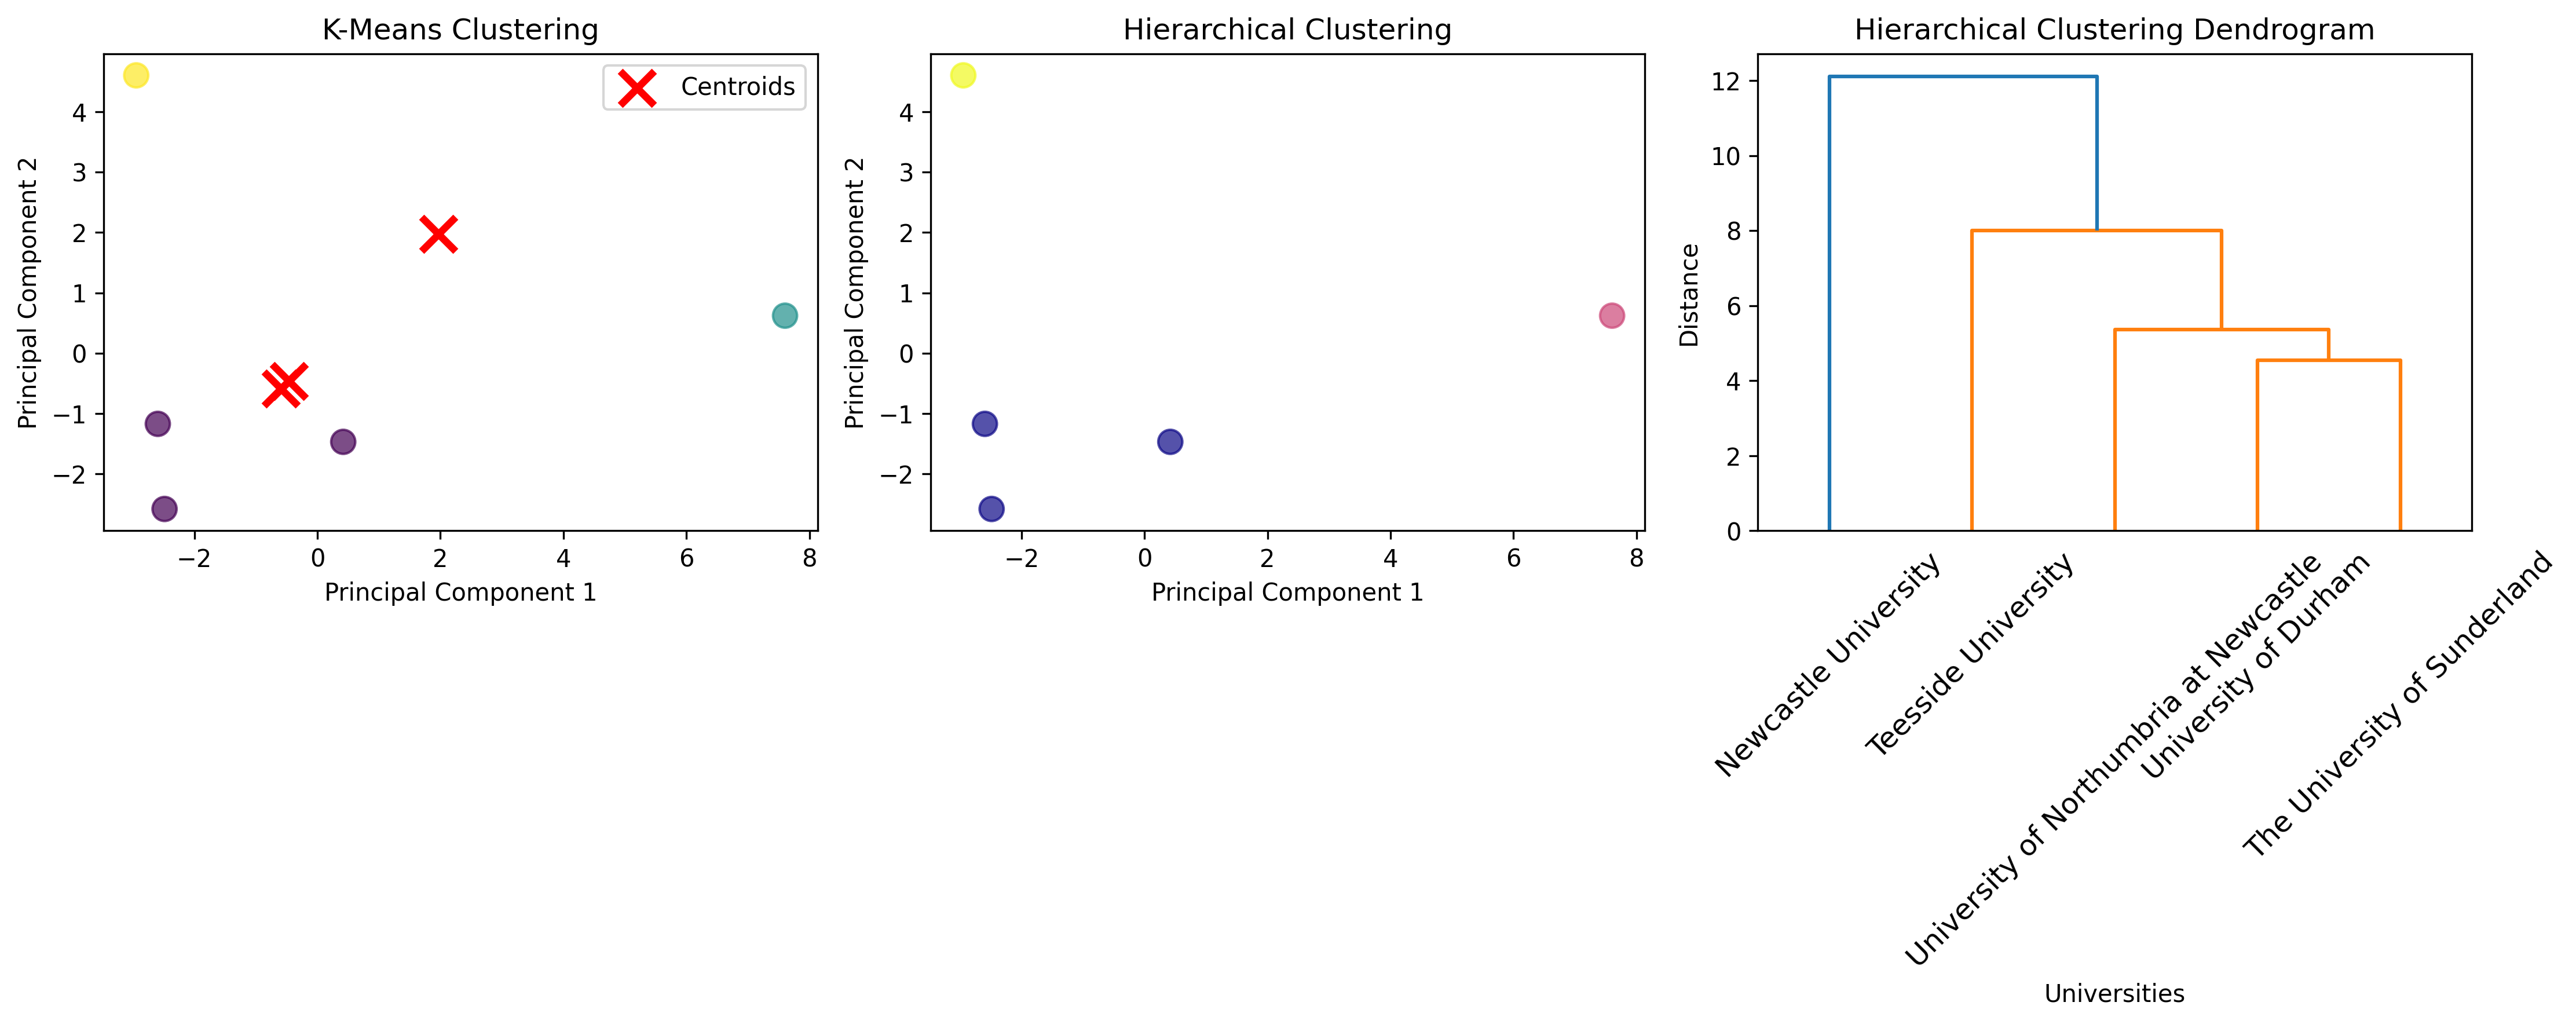
\includegraphics[width=0.9\textwidth]{Fig/figure44.clustering_analysis.png}
\caption{Clustering of Institutional Trajectories}
\label{fig:clustering-analysis}
\end{figure}

\begin{itemize}
    \item Durham consistently clusters with high-performing institutions in terms of research and CPD trend growth.
    \item Institutions such as Teesside and Sunderland group within lower-growth clusters, often marked by declining business and public engagement indicators.
    \item Newcastle shows mixed membership across clusters, aligning differently based on feature inputs. This cluster-based classification offers an intuitive view of institutional positioning, helping decision-makers benchmark progress against peers with similar trajectories.
\end{itemize}

\subsubsection{Overall Trend Performance}

Durham University's trend analysis reveals strong growth potential in research income and IP disclosures, with consistent positive forecasts across models. CPD income is also a bright spot, showing resilient and upward trends. In contrast, business income and IP income display volatility and uncertainty, pointing to potential challenges in commercialization and income stability. Public engagement, while facing projected decline, performs better than peer institutions. Overall, Durham shows solid foundations in research and innovation but needs to address monetization efficiency and business income diversification to ensure balanced, long-term growth. The trend prediction analysis presents a mixed outlook for Durham University's future performance. Research income and IP disclosures show strong growth potential across multiple prediction methods, with consistent positive trends. However, business income and IP income predictions show high volatility, indicating potential challenges in commercialization. Public engagement is predicted to decline, though at a slower rate than the national average. CPD income shows consistent positive growth predictions, suggesting potential for development in this area. The analysis suggests that while the university has strong foundations in research and IP generation, there may be challenges in commercializing these activities and maintaining business income levels.

\section{Discussion \& Recommendations for Durham University}
The comprehensive analysis reveals distinct strategic priorities for Durham University across different income streams. Based on the efficiency benchmarking, income concentration analysis, and volatility assessment, the following priority framework guides our recommendations:

\begin{itemize}
    \item \textbf{Highest Priority - Business Services Diversification:} High business services specialization\footnote{Business services specialization HHI measures the concentration of business service activities across different service types, where higher values indicate greater focus on specific service areas.} (HHI 0.47-0.69) and volatility (CV=0.380) combined with significant growth potential (+61.92\% projected) indicate the highest impact potential for diversification strategies.
    
    \item \textbf{Medium Priority - CPD Revenue Optimization:} Low CPD revenue efficiency\footnote{CPD revenue efficiency is measured as revenue per learner day, reflecting the financial return from each day of professional development delivered.} (\textsterling 0.085 per learner day) despite high learner engagement (98,190 days) suggests significant untapped potential through pricing and market strategy refinement.
    
    \item \textbf{Lower Priority - Research Funding Diversification:} Research funding volatility (CV=0.324) is primarily driven by external policy cycles rather than internal concentration, suggesting limited impact from diversification efforts.
\end{itemize}

\subsection{Income Enhancement Strategies}

\begin{itemize}
    \item \textbf{Research Income Optimization:} Durham University currently ranks 33rd nationally for research income, with \textsterling 216,850, placing it in the top 15\% of institutions. This income level surpasses the 75th percentile (\textsterling 222,681), indicating strong baseline performance. Forecasting models project further growth potential: linear regression predicts a +18.82\% increase, while exponential smoothing forecasts +26.19\%. However, a random forest model suggests a possible -7.85\% decline, highlighting the need for risk mitigation. Deep analysis reveals that Durham's research income volatility ($\mathrm{CV}=0.324$) is primarily driven by BEIS Research Councils funding concentration (60.7\% of total), creating dependency on government policy cycles, and irregular timing of large collaborative projects leading to significant year-on-year fluctuations in peak years. Recommendations include building on current momentum through targeted growth plans, implementing early-warning systems for revenue volatility, and strengthening the management of research grant applications to secure sustainable long-term growth. To address the structural volatility drivers, Durham should prioritize funding source diversification beyond BEIS Research Councils, develop multi-year grant planning to smooth project timing, and establish policy risk monitoring systems to anticipate government funding cycle changes.
      
    \item \textbf{Business Services Development:} Ranked 31st nationally, Durham's business services income shows considerable volatility, with predictions ranging from -54.84\% to +6.77\%. The HHI index (0.47-0.69) reflects high specialization, posing potential concentration risk. Further investigation reveals that Durham's business services volatility ($\mathrm{CV}=0.380$) stems from three key structural factors: (1) the dominance of contract research (64.1\% of business income) which is highly sensitive to external funding cycles, (2) the concentration of clients in non-commercial organizations (60.1\% of contracts), making the institution vulnerable to public sector budget cuts, and (3) the limited engagement with SMEs (6.3\% of contracts), missing opportunities for more stable, diversified income streams. To address this, the university should implement income stabilization mechanisms, diversify its service offerings to broaden its client base, and explore innovative business models inspired by Northumbria's projected +61.92\% growth. Specific actions include expanding SME partnerships beyond the current 6.3\% level, developing non-contract research services, and reducing non-commercial client dependency from 60.1\% to below 50\%.
    
    \item \textbf{CPD Revenue Improvement:} While Durham attracts 98,190 learner days for its CPD programs, revenue remains low at \textsterling 8,357, equating to just \textsterling 0.085 per learner day. Despite a national average decline of -26.54\%, Durham's predicted decline of -15.15\% to -15.62\% signals challenges in a declining sector. Detailed analysis uncovers the root cause of Durham's CPD underperformance: despite delivering 98,190 learner days (ranking 4th regionally), the revenue generation efficiency is extremely low at \textsterling 0.085 per learner day, compared to Teesside's \textsterling 0.211 efficiency. This inefficiency stems from (1) the high proportion of free or subsidized courses (83.1\% of total value), (2) the focus on non-commercial organizations (52.8\% of courses) which typically pay lower rates, and (3) the lack of premium CPD offerings that could command higher fees. To improve returns, the university should expand high-value CPD offerings, optimize its revenue conversion strategy, and boost its competitiveness in a declining sector. Specific actions include developing specialized, high-value professional development programs to reduce the 83.1\% free course ratio, targeting commercial organizations to increase the current 47.2\% commercial client base, and implementing tiered pricing strategies to capture higher margins from premium offerings.
\end{itemize}

\subsection{Intellectual Property Enhancement}

\begin{itemize}
    \item \textbf{IP Commercialization Strategy:} Durham's IP-related activities show significant growth potential, with IP disclosures forecasted to increase by +50.49\% and total IP income by +292.78\% (linear regression) to +194.47\% (exponential smoothing). However, the volatility in income (ranging from -46.98\% to +15.39\%) highlights the need for a more structured commercialization strategy. In-depth examination reveals that Durham's IP volatility ($\mathrm{CV}=0.676$) is fundamentally different from other institutions: while Newcastle's high volatility ($\mathrm{CV}=2.178$) stems from large, irregular licensing deals, Durham's volatility reflects a systematic commercialization challenge. Specifically, (1) only 3.7\% of licenses generate income (30 out of 808 total licenses), indicating a fundamental disconnect between IP creation and commercialization success, (2) the average income per license (\textsterling 8.28) is significantly below the national average (\textsterling 19.30), suggesting undervaluation of IP assets, and (3) the concentration in non-software licenses (85.5\% of portfolio) in a market increasingly favoring software and digital IP. The university should enhance IP protection mechanisms, establish stable and scalable commercialization pathways, and implement better portfolio-level decision-making. This analysis indicates that Durham's IP strategy requires fundamental restructuring, focusing on commercialization pipeline development rather than portfolio expansion. Specific actions include improving the income generation rate from 3.7\% to at least 5\% (national average), increasing average license value from \textsterling 8.28 to \textsterling 15.00, and developing software IP to reduce the 85.5\% non-software concentration.
    
    \item \textbf{IP Portfolio Management:} The current IP specialization level, indicated by an HHI index of 0.27-0.62, suggests moderate focus with room for optimization. Licensing activities offer a +37.06\% growth potential, and regional collaboration, particularly with high-performing neighbors like Newcastle (projected +94.45\%), should be expanded. Regular portfolio reviews and strategic alignment of underutilized assets are key to maximizing value.
\end{itemize}

\subsection{Public Engagement Enhancement}

\begin{itemize}
    \item \textbf{Engagement Strategy Development:} Durham ranks 31st nationally in public engagement, with a total activity value of \textsterling 6,043,792. However, 72.1\% of events are free, limiting revenue generation. Forecasts predict a -20.35\% decline in overall engagement value, better than the national average of -30.30\%, but still significant. To adapt, Durham should rebalance its mix of free and chargeable events and explore new outreach models, taking cues from Teesside's projected +24.90\% growth.
    
    \item \textbf{Resource Optimization:} The university recorded 6,024,744 participants and 19,048 days of academic staff engagement, indicating a need for efficiency improvements. Strategies should focus on optimizing resource allocation to high-impact events, improving staff time utilization, and tightening cost control processes to protect against sector-wide contraction.
\end{itemize}

\subsection{Regional Leadership Development}

\begin{itemize}
    \item \textbf{Regional Position Strengthening:} Durham maintains the second-highest overall performance in the North East, supported by a research HHI index of 0.28-0.31, which reflects healthy diversification. To consolidate and expand this regional leadership, the university should narrow its income gap with Newcastle, enhance the impact of diversified research streams, and leverage growth opportunities such as Northumbria's forecasted +39.25\% increase in regional activity.
    
    \item \textbf{Specialization Strategy:} The university should continue to maintain moderate specialization in research while optimizing its business service and IP activity focus areas. A balanced specialization approach can support both institutional stability and regional distinctiveness, aligning with broader strategic goals.
\end{itemize}

\subsection{Efficiency Enhancement Strategies}

\begin{itemize}
    \item \textbf{Optimize Input-Output Ratios:} Durham's efficiency in research and IP income is commendable but CPD and business service efficiency remain suboptimal. The efficiency gap is quantifiable across different metrics: Durham's CPD revenue generation efficiency\footnote{CPD revenue efficiency is measured as revenue per learner day, reflecting the financial return from each day of professional development delivered.} (\textsterling 0.085 per learner day) is only 40.3\% of Teesside's efficiency (\textsterling 0.211 per learner day), while Durham's business services efficiency\footnote{Business services efficiency is measured as income per academic staff day, reflecting the productivity of staff time invested in business activities.} (\textsterling 27.73 per staff day) is 43.0\% of Newcastle's efficiency (\textsterling 64.44 per staff day). Benchmarking against Newcastle's CPD monetization and Teesside's business services model can inform better conversion practices. Specific efficiency targets should include increasing CPD revenue efficiency from \textsterling 0.085 to \textsterling 0.150 per learner day (76.5\% improvement), and business services efficiency from \textsterling 27.73 to \textsterling 40.00 per staff day (44.3\% improvement), based on regional best practices.
    
    \item \textbf{Allocate Resources Based on ROI Profiles:} Departments and services should be assessed based on their efficiency metrics. Low-efficiency areas could be restructured or supported with performance-based incentives to encourage revenue-focused practices.
    
    \item \textbf{Institutionalize Efficiency Monitoring:} Establishing a KPI dashboard to track per-unit revenue generation and investment efficiency will allow administrators to react proactively to declining performance in specific sectors.
\end{itemize}

\subsection{Resilience Improvement Strategies}

\begin{itemize}
    \item \textbf{Volatility Buffering in High-Risk Streams:} For business income and spin-out companies, which show the highest volatility, Durham should explore diversification strategies, long-term partnerships, and multi-year contracts to smooth income cycles. The volatility risk is quantifiable: business services show the highest volatility (CV=0.380) and concentration (HHI 0.47-0.69), while research income shows moderate volatility (CV=0.309). Durham should prioritize business service diversification to reduce concentration risk and volatility, while maintaining research funding diversity through policy risk monitoring.
    
    \item \textbf{Scenario Stress Testing:} A simulation-based risk assessment framework should be implemented to project financial performance under varying policy and funding scenarios, particularly for entrepreneurial units.
    
    \item \textbf{Strengthen Institutional Slack:} Build financial and staffing buffers in units that historically show high variance. This includes maintaining reserve funds or cross-subsidizing critical but volatile streams.
\end{itemize}

\subsection{Future Development Priorities}

\begin{itemize}
    \item \textbf{Short-term Priorities (1-2 years):} Immediate actions should include stabilizing business services income, improving CPD revenue conversion, refining public engagement structures, and enhancing IP commercialization frameworks to increase early returns.
    
    \item \textbf{Medium-term Priorities (3-5 years):} Over the medium term, Durham should scale up its research income, develop stable IP revenue models, refine public engagement into a revenue-contributing activity, and further strengthen its role as a regional leader in innovation and collaboration.
    
    \item \textbf{Long-term Priorities (5+ years):} In the long run, Durham should aim to elevate its national standing, establish robust and sustainable income streams across all categories, build international partnerships, and solidify its influence both regionally and globally.
\end{itemize}

Detailed Implementation Timeline:

\begin{itemize}
    \item \textbf{Short-term (1-2 years):} In addition to stabilizing business services and enhancing IP commercialization, immediate focus should be placed on improving CPD efficiency and reducing year-on-year volatility in high-risk categories through contingency planning and contract stabilization.
    
    \item \textbf{Medium-term (3-5 years):} Develop an institutional data-driven forecasting system combining model ensemble predictions with historical volatility to guide medium-term investment. Strengthen efficiency in underperforming segments via performance-linked budgeting and better ROI tracking.
    
    \item \textbf{Long-term (5+ years):} Move towards becoming a national leader in institutional resilience and predictive management. Establish an integrated strategic planning unit that links forecasting, risk analysis, and financial planning into a coherent framework for long-term stability and growth.
\end{itemize}

\section{Conclusion}

This comprehensive analysis of Durham University's HE-BCI performance reveals a complex institutional profile characterized by both significant strengths and strategic challenges within the UK higher education landscape. The study demonstrates that Durham maintains a strong regional position as the second-highest performing institution in the North East, consistently ranking among the top 15\% nationally across multiple performance indicators. The university's research income performance is particularly noteworthy, with \textsterling 216,850 placing it 33rd nationally and significantly outperforming the national average by \textsterling 87,327.

The analysis identifies several key strengths that position Durham for continued success. The university demonstrates robust IP generation capabilities, ranking 31st nationally in disclosures with a substantial patent portfolio of 2,019 patents and supporting 642 active spin-off companies that employ 5,455 FTE staff and generate \textsterling 542.35 million in turnover. Public engagement activities show significant community impact, with 6,024,744 participants across diverse programming, though 72.1\% of events are free, limiting revenue generation. Regional positioning analysis reveals balanced specialization with HHI values of 0.28-0.31 in research, indicating healthy diversification without overconcentration.

However, the study also reveals critical areas requiring strategic attention. Performance efficiency analysis shows that Durham underperforms relative to peers when normalized by academic staff time, ranking 78th nationally in research efficiency and 95th in business services efficiency. Business services income shows considerable volatility (CV=0.380), primarily due to high dependency on contract research (64.1\% of business income) and non-commercial organizations (60.1\% of clients). IP commercialization efficiency remains low, with only 3.7\% of licenses generating income, significantly below the national average of \textsterling 19.30 per license. CPD activities, despite high learner engagement (98,190 days), generate minimal revenue (\textsterling 0.085 per learner day), indicating substantial untapped potential compared to regional peers like Teesside (\textsterling 0.211 per learner day).

The trend prediction analysis offers a mixed outlook for Durham's future performance. Research income and IP disclosures show strong growth potential (+18.82\% to +26.19\% and +50.49\% respectively), while CPD income trends show decline (-15.15\% to -15.62\%) across all models. However, business income projections show high volatility (-54.84\% to +6.77\%), highlighting the urgent need for stabilization strategies. Public engagement is predicted to decline by -20.35\%, though this is significantly better than the national average of -30.30\%.

To address these challenges and capitalize on opportunities, Durham should prioritize business service diversification as its highest strategic priority, targeting a 40-60\% reduction in volatility through expanded SME partnerships and reduced non-commercial client dependency. IP commercialization requires fundamental restructuring to improve income generation rates from 3.7\% to at least 5\%, while CPD optimization should focus on premium offerings and commercial client expansion to improve efficiency from \textsterling 0.085 to \textsterling 0.150 per learner day.

The analysis demonstrates that Durham University possesses the foundational strengths necessary for continued regional leadership and national prominence. By implementing the identified strategic priorities, particularly in business diversification, IP commercialization, and efficiency optimization, Durham can enhance its resilience, improve income stability, and strengthen its position as a key driver of innovation and economic development in the North East region.

\appendix

\section{Data Sources and Script References}

This appendix provides a comprehensive reference table listing all key data points, metrics, and statistics used throughout the report, along with their corresponding analysis scripts and source CSV files. This table serves as a complete data provenance record for transparency and reproducibility.

\vspace{0.3cm}
\begin{table}[h]
\centering
\caption{Complete Data Sources and Script References}
\vspace{0.1cm}
\resizebox{0.99\textwidth}{!}{%
\begin{tabular}{|l|l|l|l|l|}
\hline \textbf{Data Point/Metric} & \textbf{Value} & \textbf{National Rank} & \textbf{Analysis Script} & \textbf{Source CSV} \\
\hline \multicolumn{5}{|l|}{\textbf{Income Analysis (Section~\ref{sec:income-analysis})}} \\
\hline Durham Research Income & £216,850 & 33/228 & 2.income\_analysis.py & table-1.csv \\
\hline National Average Research Income & £129,523 & - & 2.income\_analysis.py & table-1.csv \\
\hline Durham Business Services Income & £157,635 & 40/228 & 2.income\_analysis.py & table-2a.csv \\
\hline National Average Business Services & £96,333 & - & 2.income\_analysis.py & table-2a.csv \\
\hline Durham CPD Income & £8,357 & 123/228 & 2.income\_analysis.py & table-2b.csv \\
\hline National Average CPD Income & £30,026 & - & 2.income\_analysis.py & table-2b.csv \\
\hline Durham Regeneration Income & £13,272 & 52/228 & 2.income\_analysis.py & table-3.csv \\
\hline National Average Regeneration & £10,865 & - & 2.income\_analysis.py & table-3.csv \\
\hline Durham Total Income & £396,114 & 2/5 (Regional) & 2.income\_analysis.py & Multiple tables \\
\hline \multicolumn{5}{|l|}{\textbf{Intellectual Property Analysis (Section~\ref{sec:ip-analysis})}} \\
\hline Durham IP Disclosures & 3,458 & 28/228 & 3.ip\_analysis.py & table-4a.csv \\
\hline National Average IP Disclosures & 2,076 & - & 3.ip\_analysis.py & table-4a.csv \\
\hline Durham Patent Portfolio & 2,019 & - & 3.ip\_analysis.py & table-4a.csv \\
\hline Durham New Patent Applications & 124 & - & 3.ip\_analysis.py & table-4a.csv \\
\hline Durham Patents Granted & 80 & - & 3.ip\_analysis.py & table-4a.csv \\
\hline Durham Total Licenses & 808 & 35/228 & 3.ip\_analysis.py & table-4b.csv \\
\hline National Average Licenses & 2,258 & - & 3.ip\_analysis.py & table-4b.csv \\
\hline Durham Income-Generating Licenses & 30 & - & 3.ip\_analysis.py & table-4b.csv \\
\hline Durham IP Income & £6,687 & 34/228 & 3.ip\_analysis.py & table-4d.csv \\
\hline National Average IP Income & £10,803 & - & 3.ip\_analysis.py & table-4d.csv \\
\hline Durham Active Spin-off Companies & 642 & 25/228 & 3.ip\_analysis.py & table-4e.csv \\
\hline Durham Spin-off Employment (FTE) & 5,455 & - & 3.ip\_analysis.py & table-4e.csv \\
\hline Durham Spin-off Turnover & £542.35M & - & 3.ip\_analysis.py & table-4e.csv \\
\hline Durham Spin-off External Investment & £117.66M & - & 3.ip\_analysis.py & table-4e.csv \\
\hline \multicolumn{5}{|l|}{\textbf{Public Engagement Analysis (Section~\ref{sec:public-engagement})}} \\
\hline Durham Total Engagement Events & 6,043,792 & 31/228 & 4.public\_engagement\_analysis.py & table-5.csv \\
\hline National Average Engagement Events & 29,012,765 & - & 4.public\_engagement\_analysis.py & table-5.csv \\
\hline Durham Total Participants & 6,024,744 & - & 4.public\_engagement\_analysis.py & table-5.csv \\
\hline Durham Academic Staff Time (Days) & 19,048 & - & 4.public\_engagement\_analysis.py & table-5.csv \\
\hline Durham Free Events Percentage & 72.1\% & - & 4.public\_engagement\_analysis.py & table-5.csv \\
\hline Durham Chargeable Events & 1,687,130 & - & 4.public\_engagement\_analysis.py & table-5.csv \\
\hline Durham Free Events & 4,356,662 & - & 4.public\_engagement\_analysis.py & table-5.csv \\
\hline \multicolumn{5}{|l|}{\textbf{Performance Efficiency Analysis (Section~\ref{sec:performance-efficiency})}} \\
\hline Durham Research Efficiency & £19.76/staff day & 78/227 & 6.performance\_efficiency\_analysis.py & table-1.csv + staff data \\
\hline Durham Business Efficiency & £27.73/staff day & 95/228 & 6.performance\_efficiency\_analysis.py & table-2a.csv + staff data \\
\hline Durham IP Efficiency & £0.44/staff day & 71/228 & 6.performance\_efficiency\_analysis.py & table-4d.csv + staff data \\
\hline Durham CPD Efficiency & £0.64/staff day & 162/228 & 6.performance\_efficiency\_analysis.py & table-2b.csv + staff data \\
\hline Newcastle Research Efficiency & £117.35/staff day & 29/227 & 6.performance\_efficiency\_analysis.py & table-1.csv + staff data \\
\hline Newcastle Business Efficiency & £64.44/staff day & 60/228 & 6.performance\_efficiency\_analysis.py & table-2a.csv + staff data \\
\hline Newcastle IP Efficiency & £3.02/staff day & 35/228 & 6.performance\_efficiency\_analysis.py & table-4d.csv + staff data \\
\hline Newcastle CPD Efficiency & £2.21/staff day & 140/228 & 6.performance\_efficiency\_analysis.py & table-2b.csv + staff data \\
\hline \multicolumn{5}{|l|}{\textbf{Resilience and Risk Analysis (Section~\ref{sec:resilience-risk})}} \\
\hline Durham Research Income CV & 0.324 & 58/228 & 7.resilience\_risk\_analysis.py & table-1.csv \\
\hline Durham Business Services CV & 0.380 & 108/228 & 7.resilience\_risk\_analysis.py & table-2a.csv \\
\hline Durham CPD Income CV & 0.340 & 84/228 & 7.resilience\_risk\_analysis.py & table-2b.csv \\
\hline Durham IP Income CV & 2.408 & 121/228 & 7.resilience\_risk\_analysis.py & table-4d.csv \\
\hline Newcastle Research Income CV & 0.125 & 7/228 & 7.resilience\_risk\_analysis.py & table-1.csv \\
\hline Newcastle Business Services CV & 0.085 & 9/228 & 7.resilience\_risk\_analysis.py & table-2a.csv \\
\hline Newcastle CPD Income CV & 0.290 & - & 7.resilience\_risk\_analysis.py & table-2b.csv \\
\hline Newcastle IP Income CV & 2.150 & 119/228 & 7.resilience\_risk\_analysis.py & table-4d.csv \\
\hline Durham Research HHI & 0.28-0.31 & - & 7.resilience\_risk\_analysis.py & table-1.csv \\
\hline Durham Business Services HHI & 0.47-0.69 & - & 7.resilience\_risk\_analysis.py & table-2a.csv \\
\hline Durham IP HHI & 0.27-0.62 & - & 7.resilience\_risk\_analysis.py & table-4d.csv \\
\hline \multicolumn{5}{|l|}{\textbf{Trend Prediction Analysis (Section~\ref{sec:analysis-results})}} \\
\hline Durham Research Income Growth (Linear) & +25.70\% & - & 8.trend\_prediction.py & table-1.csv \\
\hline Durham Research Income Growth (Exp Smooth) & +27.04\% & - & 8.trend\_prediction.py & table-1.csv \\
\hline Durham Research Income Growth (Random Forest) & -5.63\% & - & 8.trend\_prediction.py & table-1.csv \\
\hline Durham Business Income Growth (Linear) & -54.84\% & - & 8.trend\_prediction.py & table-2a.csv \\
\hline Durham Business Income Growth (Exp Smooth) & -31.56\% & - & 8.trend\_prediction.py & table-2a.csv \\
\hline Durham Business Income Growth (Random Forest) & +6.77\% & - & 8.trend\_prediction.py & table-2a.csv \\
\hline Durham CPD Income Growth (All Models) & +39.28\% & - & 8.trend\_prediction.py & table-2b.csv \\
\hline Durham IP Disclosures Growth & +50.49\% & - & 8.trend\_prediction.py & table-4a.csv \\
\hline Durham IP Income Growth (Linear) & -47.71\% & - & 8.trend\_prediction.py & table-4d.csv \\
\hline Durham IP Income Growth (Random Forest) & +15.39\% & - & 8.trend\_prediction.py & table-4d.csv \\
\hline Durham Public Engagement Growth & -20.35\% & - & 8.trend\_prediction.py & table-5.csv \\
\hline National Average Public Engagement Growth & -30.30\% & - & 8.trend\_prediction.py & table-5.csv \\
\hline \multicolumn{5}{|l|}{\textbf{Dataset Overview (Section~\ref{sec:methodology})}} \\
\hline Total Institutions in Dataset & 228 & - & 1.data\_exploratory\_analysis.py & All tables \\
\hline Time Period Covered & 2014/15-2023/24 & - & 1.data\_exploratory\_analysis.py & All tables \\
\hline North East Institutions & 5 & - & 1.data\_exploratory\_analysis.py & All tables \\
\hline Missing Values Table 1 & 25 & - & 1.data\_exploratory\_analysis.py & table-1.csv \\
\hline Missing Values Table 2a & 22,500 & - & 1.data\_exploratory\_analysis.py & table-2a.csv \\
\hline Missing Values Table 2b & 5 & - & 1.data\_exploratory\_analysis.py & table-2b.csv \\
\hline Missing Values Table 3 & 1,452 & - & 1.data\_exploratory\_analysis.py & table-3.csv \\
\hline Missing Values Table 4c & 9 & - & 1.data\_exploratory\_analysis.py & table-4c.csv \\
\hline Missing Values Table 4d & 5 & - & 1.data\_exploratory\_analysis.py & table-4d.csv \\
\hline Missing Values Table 4e & 10 & - & 1.data\_exploratory\_analysis.py & table-4e.csv \\
\hline Missing Values Table 5 & 0 & - & 1.data\_exploratory\_analysis.py & table-5.csv \\
\hline
\end{tabular}
}
\label{tab:data-sources-complete}
\end{table}

\vspace{0.3cm}
\textbf{Notes:}
\begin{itemize}
    \item \textbf{CV:} Coefficient of Variation, measuring income volatility
    \item \textbf{HHI:} Herfindahl-Hirschman Index, measuring income concentration/diversification
    \item \textbf{FTE:} Full-Time Equivalent employment
    \item \textbf{Regional Rank:} Position among the 5 North East institutions
    \item \textbf{National Rank:} Position among all 228 UK higher education institutions
    \item \textbf{Staff Data:} Academic staff time data used for efficiency calculations derived from HE-BCI survey metadata
    \item \textbf{Multiple Tables:} Some metrics require data from multiple CSV files for comprehensive analysis
\end{itemize}

% \section{Forecasted Trends and Additional Results}

% This appendix contains additional forecasting results and trend analysis data that support the main findings presented in the report. The script overview as follows,
% \begin{itemize}
%     \item \textbf{Data Exploratory Analysis (1.data\_exploratory\_analysis.py):} Initial data exploration, missing value analysis, and dataset overview visualizations
%     \item \textbf{Income Analysis (2.income\_analysis.py):} Comprehensive analysis of research income, business services, CPD, and regeneration income
%     \item \textbf{IP Analysis (3.ip\_analysis.py):} Intellectual property disclosures, licensing, and commercialization analysis
%     \item \textbf{Public Engagement (4.public\_engagement\_analysis.py):} Public engagement activities, events, and community interaction analysis
%     \item \textbf{Regional Analysis (5.extral\_regional\_analysis.py):} Regional comparison and specialization analysis using HHI indices
%     \item \textbf{Performance Efficiency (6.performance\_efficiency\_analysis.py):} Efficiency metrics and benchmarking analysis
%     \item \textbf{Resilience Risk (7.resilience\_risk\_analysis.py):} Volatility analysis, coefficient of variation calculations, and risk assessment
%     \item \textbf{Trend Prediction (8.trend\_prediction.py):} Advanced forecasting models including linear regression, exponential smoothing, random forest, ARIMA, and XGBoost
% \end{itemize}

% All scripts use Python 3.10 with pandas, matplotlib, numpy, and scikit-learn libraries. The code includes comprehensive error handling, logging, and produces publication-ready visualizations with consistent styling. The following are excerpts of key code from each analysis module.

% 1. Data Exploratory Analysis Script:
% \inputminted{python}{Code/1.data_exploratory_analysis.py}

% 2. Income Analysis Script:
% \inputminted{python}{Code/2.income_analysis.py}

% 3. IP Analysis Script:
% \inputminted{python}{Code/3.ip_analysis.py}

% 4. Public Engagement Analysis Script:
% \inputminted{python}{Code/4.public_engagement_analysis.py}

% 5. Regional Analysis Script:
% \inputminted{python}{Code/5.extral_regional_analysis.py}

% 6. Performance Efficiency Analysis Script:
% \inputminted{python}{Code/6.performance_efficiency_analysis.py}

% 7. Resilience Risk Analysis Script:
% \inputminted{python}{Code/7.resilience_risk_analysis.py}

% 8. Trend Prediction Script:
% \inputminted{python}{Code/8.trend_prediction.py}

\vspace{0.3cm}
\begin{table}[h]
\centering
\caption{Forecasted Trends by Model and Institution (\% Change from Last Observed Year)}
\resizebox{0.99\textwidth}{!}{%
\begin{tabular}{|l|l|l|l|l|l|}
\hline \textbf{Institution} & \textbf{Model} & \textbf{Research Income} & \textbf{Business Income} & \textbf{Total IP Income} & \textbf{Spin-out Companies} \\
\hline National Average & Linear Regression & -2.33\% & -11.64\% & +16.25\% & +46.64\% \\
\hline National Average & Exponential Smoothing & -1.75\% & -11.64\% & +16.25\% & +46.64\% \\
\hline National Average & Random Forest & -4.52\% & -5.33\% & -3.81\% & +13.82\% \\
\hline National Average & ARIMA & -8.66\% & -9.73\% & -11.00\% & -34.67\% \\
\hline National Average & XGBoost & -14.65\% & -19.26\% & -12.35\% & -0.14\% \\
\hline University of Durham & Linear Regression & +18.82\% & -54.84\% & +292.78\% & -9.18\% \\
\hline University of Durham & Exponential Smoothing & +26.19\% & -31.56\% & +194.47\% & -9.18\% \\
\hline University of Durham & Random Forest & -7.85\% & +6.77\% & +15.39\% & +3.11\% \\
\hline University of Durham & ARIMA & -18.43\% & +15.88\% & +803.65\% & -0.67\% \\
\hline University of Durham & XGBoost & -21.47\% & +2.41\% & +0.17\% & +11.60\% \\
\hline Newcastle University & Linear Regression & +2.52\% & -8.47\% & +94.45\% & +36.39\% \\
\hline Newcastle University & Exponential Smoothing & +10.81\% & -1.15\% & +94.45\% & +36.39\% \\
\hline Newcastle University & Random Forest & -3.14\% & +0.25\% & -6.78\% & -29.04\% \\
\hline Newcastle University & ARIMA & -14.66\% & -5.55\% & +127.58\% & -29.04\% \\
\hline Newcastle University & XGBoost & -0.02\% & -15.65\% & -16.20\% & -0.10\% \\
\hline Northumbria University at Newcastle & Linear Regression & +39.30\% & +61.92\% & -22.19\% & +5.02\% \\
\hline Northumbria University at Newcastle & Exponential Smoothing & +26.21\% & +61.92\% & -22.19\% & +5.02\% \\
\hline Northumbria University at Newcastle & Random Forest & -2.39\% & +14.36\% & -9.01\% & -12.54\% \\
\hline Northumbria University at Newcastle & ARIMA & -8.35\% & +2.61\% & -40.11\% & -12.54\% \\
\hline Northumbria University at Newcastle & XGBoost & -0.01\% & -0.00\% & -47.71\% & -0.17\% \\
\hline Teesside University & Linear Regression & -10.61\% & -25.22\% & n/a & +31.95\% \\
\hline Teesside University & Exponential Smoothing & +136.16\% & -11.46\% & n/a & +31.95\% \\
\hline Teesside University & Random Forest & -18.77\% & +1.29\% & n/a & -27.27\% \\
\hline Teesside University & ARIMA & +105.99\% & +2.49\% & n/a & -27.27\% \\
\hline Teesside University & XGBoost & -0.36\% & -0.00\% & n/a & -0.19\% \\
\hline University of Sunderland & Linear Regression & -64.32\% & +3.71\% & -102.36\% & +18.52\% \\
\hline University of Sunderland & Exponential Smoothing & -31.65\% & +3.71\% & -102.36\% & +18.52\% \\
\hline University of Sunderland & Random Forest & -30.82\% & -9.17\% & -41.00\% & -19.35\% \\
\hline University of Sunderland & ARIMA & -7.61\% & -22.30\% & -71.30\% & -19.35\% \\
\hline University of Sunderland & XGBoost & -0.02\% & -0.69\% & -0.51\% & -15.43\% \\
\hline
\end{tabular}
}
\label{tab:forecasted-trends}
\end{table}

\begin{figure}[h]
\centering
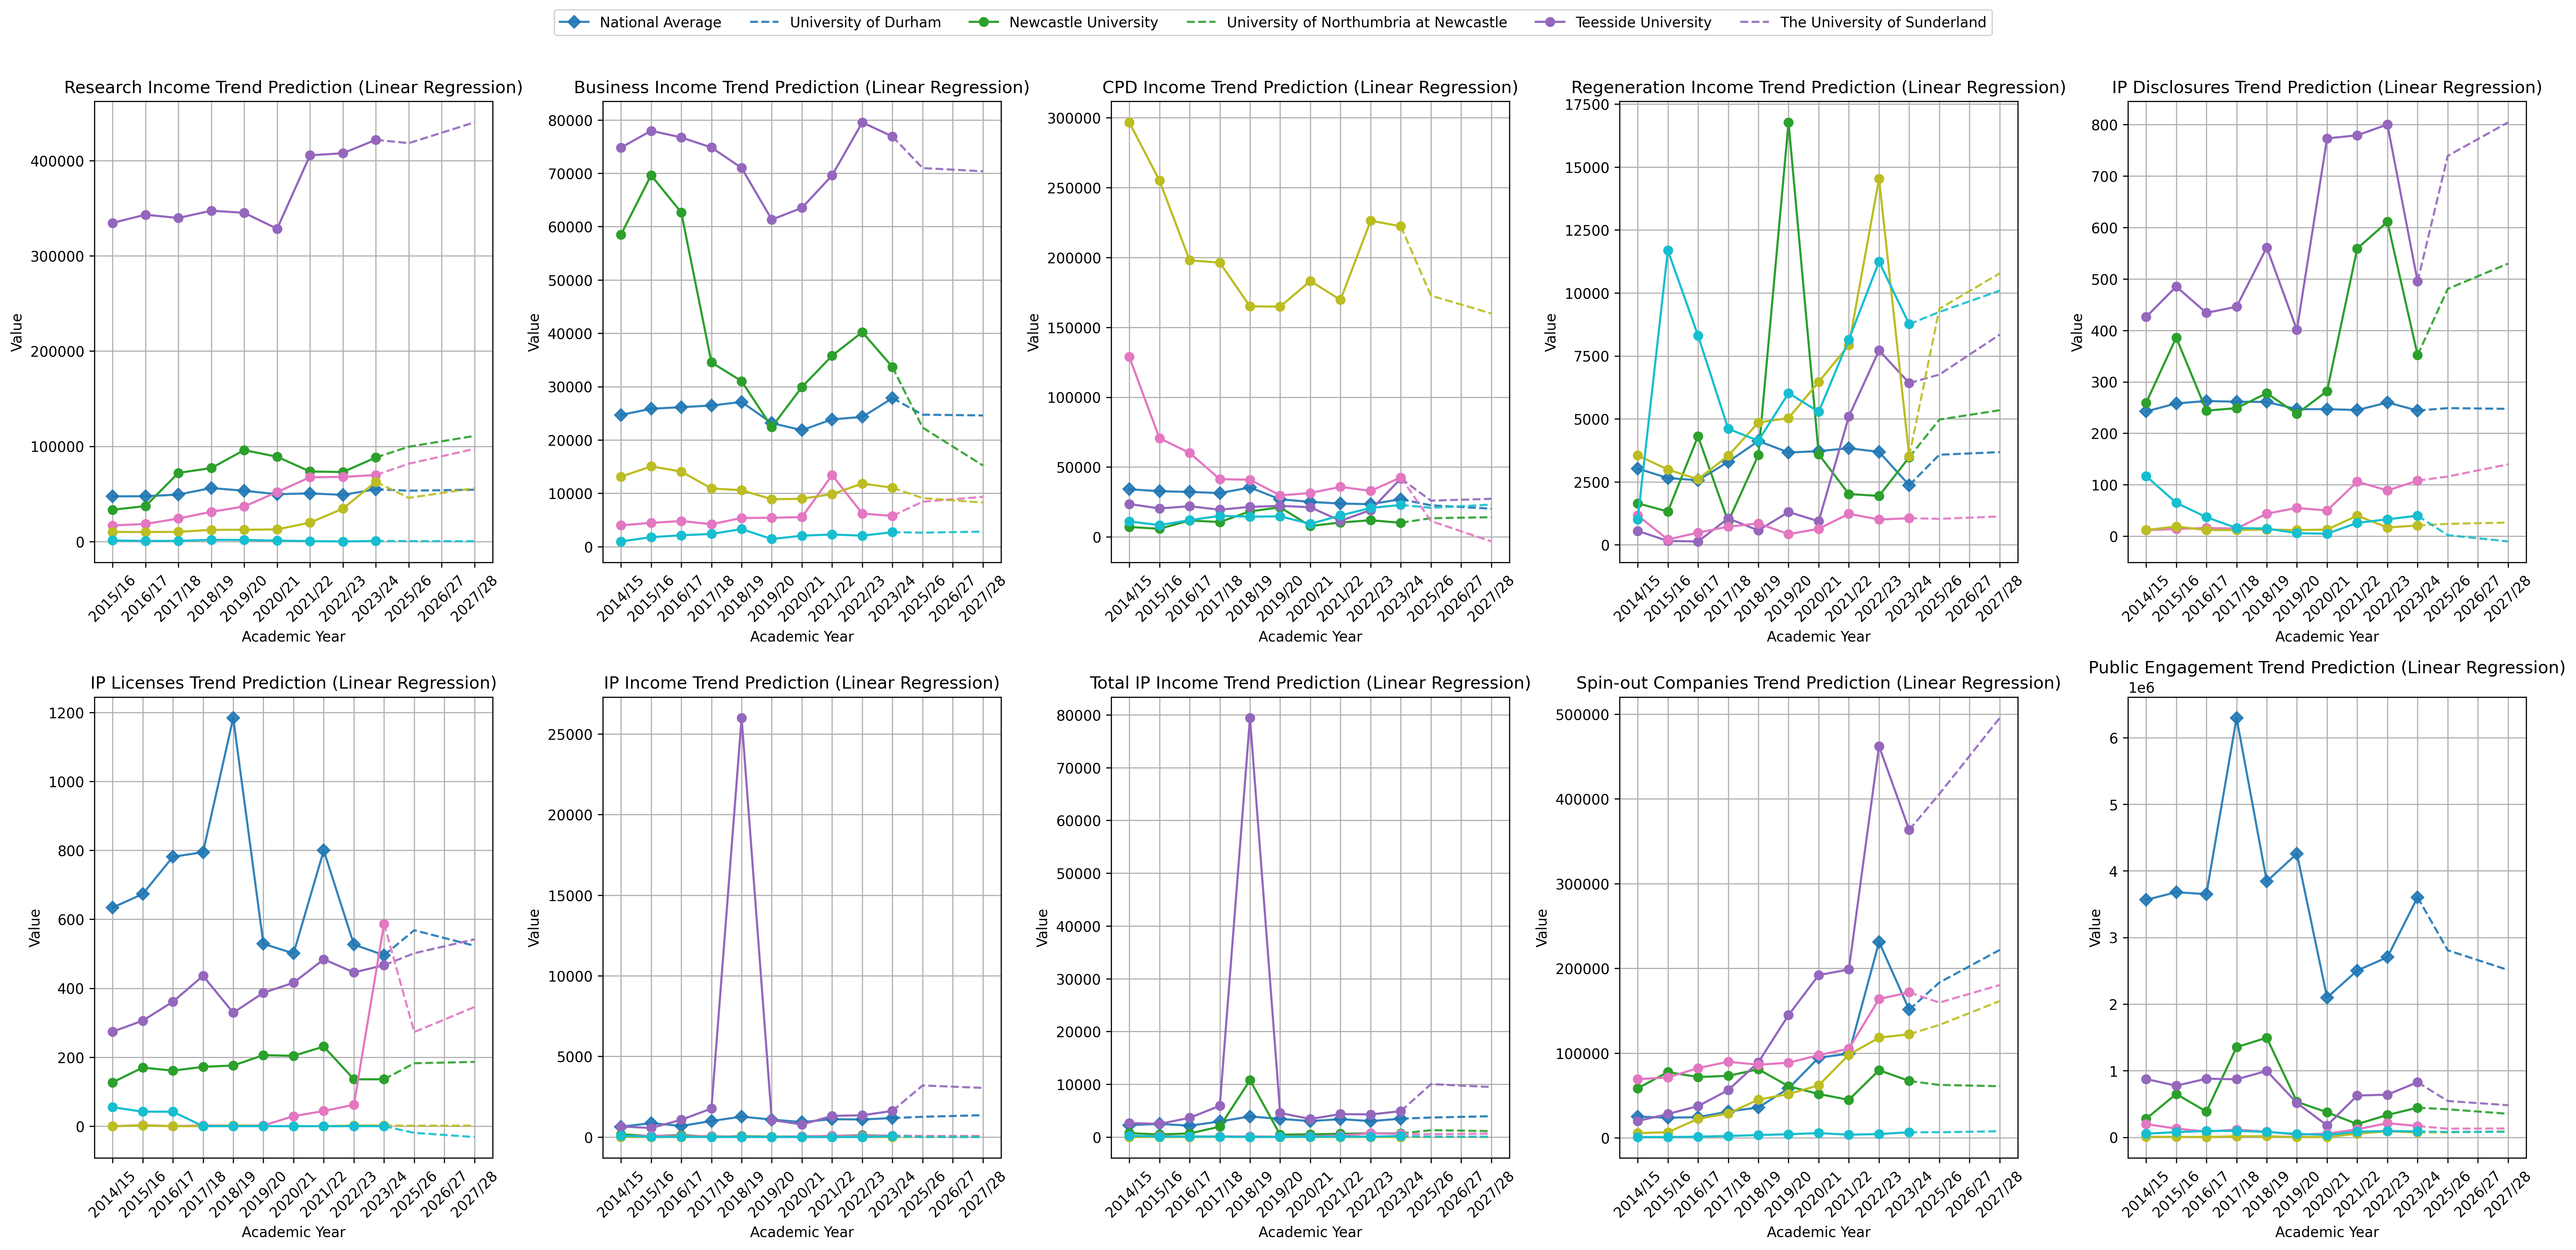
\includegraphics[width=0.95\textwidth]{Fig/appendix2.trend_predictions_linear_regression.png}
\caption{Trend predictions linear regression}
\label{fig:trend-predictions-linear-regression}
\end{figure}

\begin{figure}[h]
\centering
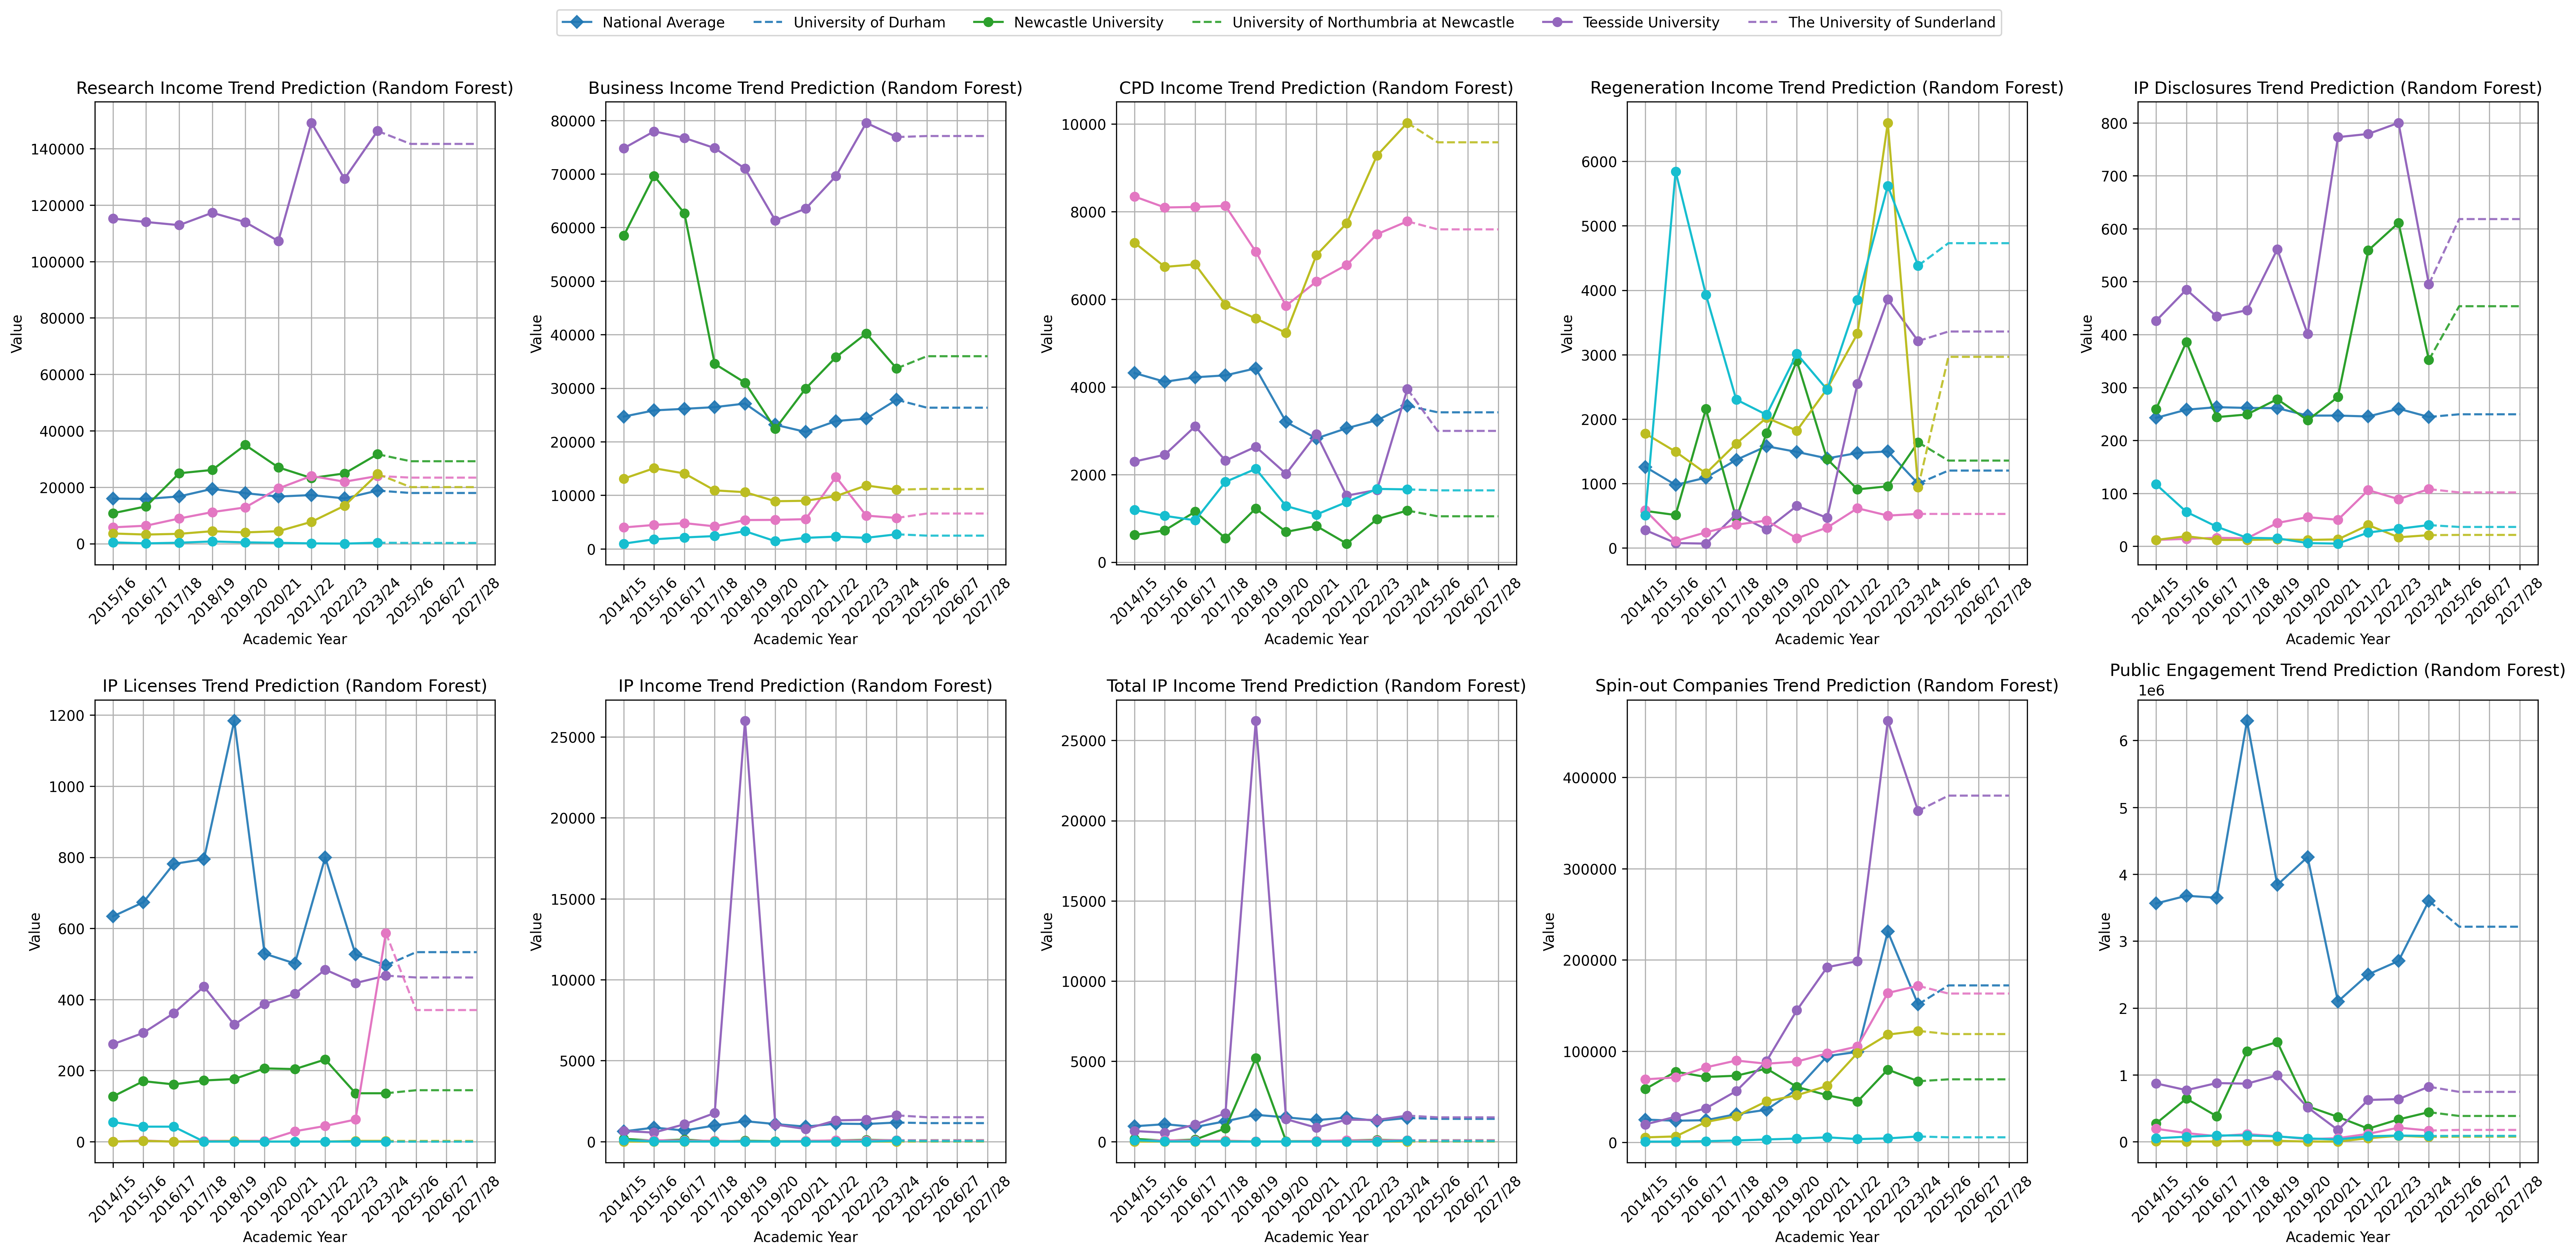
\includegraphics[width=0.95\textwidth]{Fig/appendix3.trend_predictions_random_forest.png}
\caption{Trend predictions random forest}
\label{fig:trend-predictions-random-forest}
\end{figure}

\begin{figure}[h]
\centering
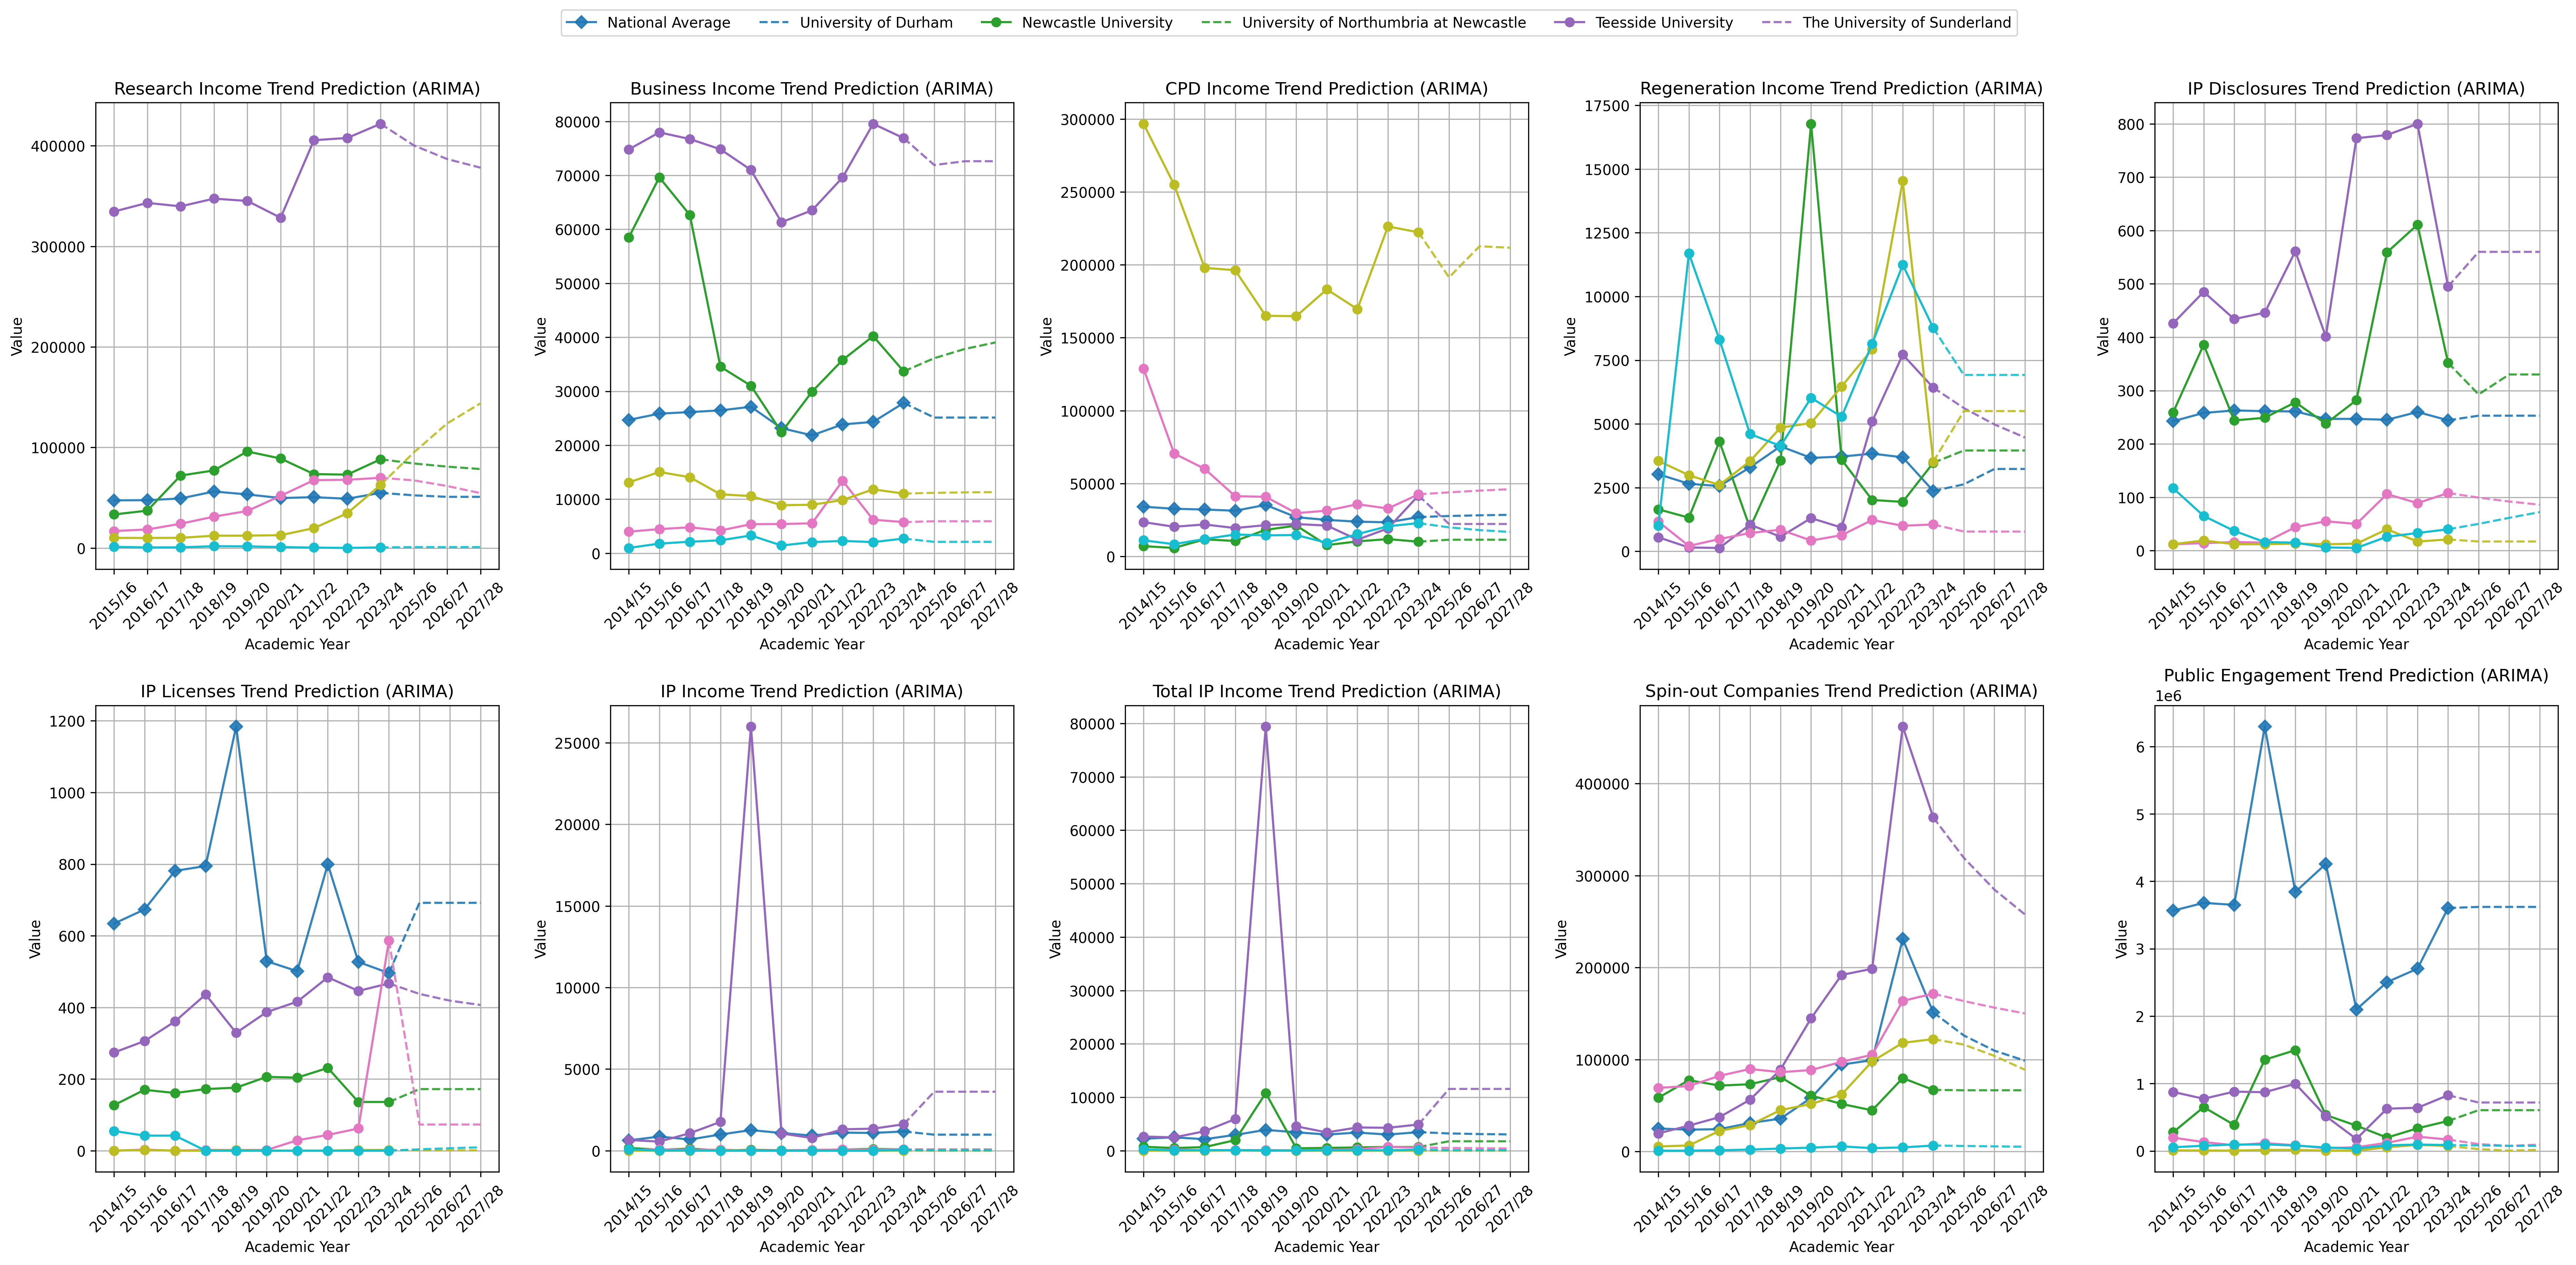
\includegraphics[width=0.95\textwidth]{Fig/appendix1.trend_predictions_arima.png}
\caption{Trend predictions ARIMA}
\label{fig:trend-predictions-arima}
\end{figure}

\begin{figure}[h]
\centering
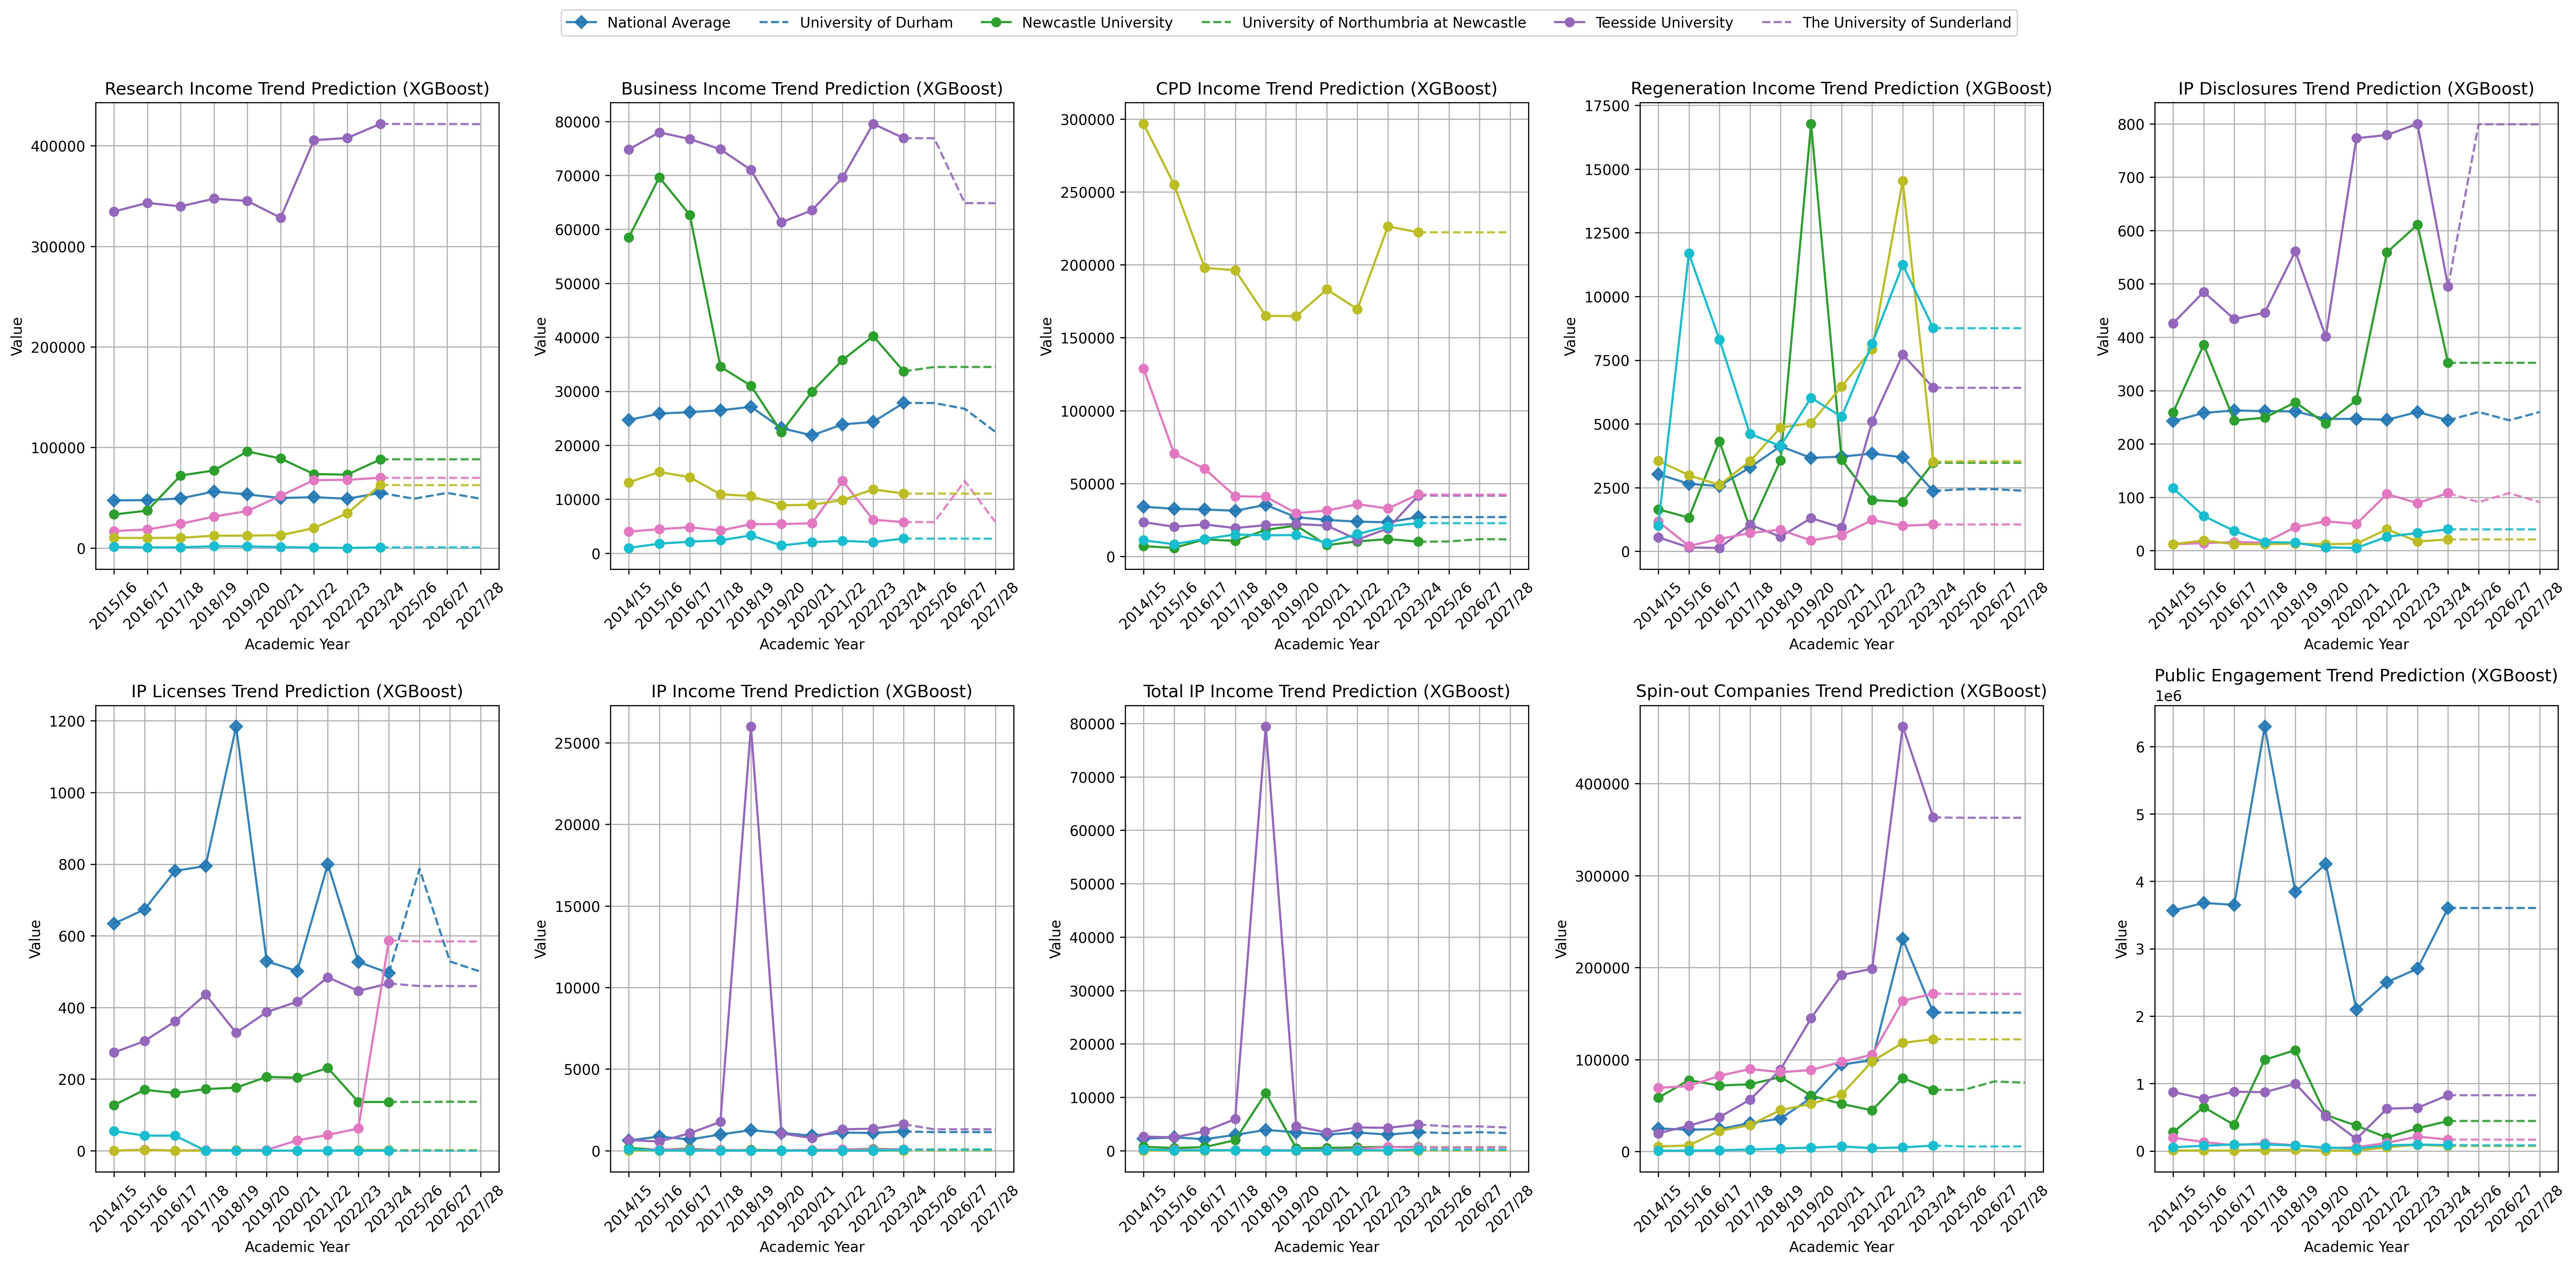
\includegraphics[width=0.95\textwidth]{Fig/appendix4.trend_predictions_xgboost.png}
\caption{Trend predictions XGBoost}
\label{fig:trend-predictions-xgboost}
\end{figure}

\begin{figure}[h]
    \centering
    \begin{subfigure}[b]{0.48\textwidth}
        \centering
        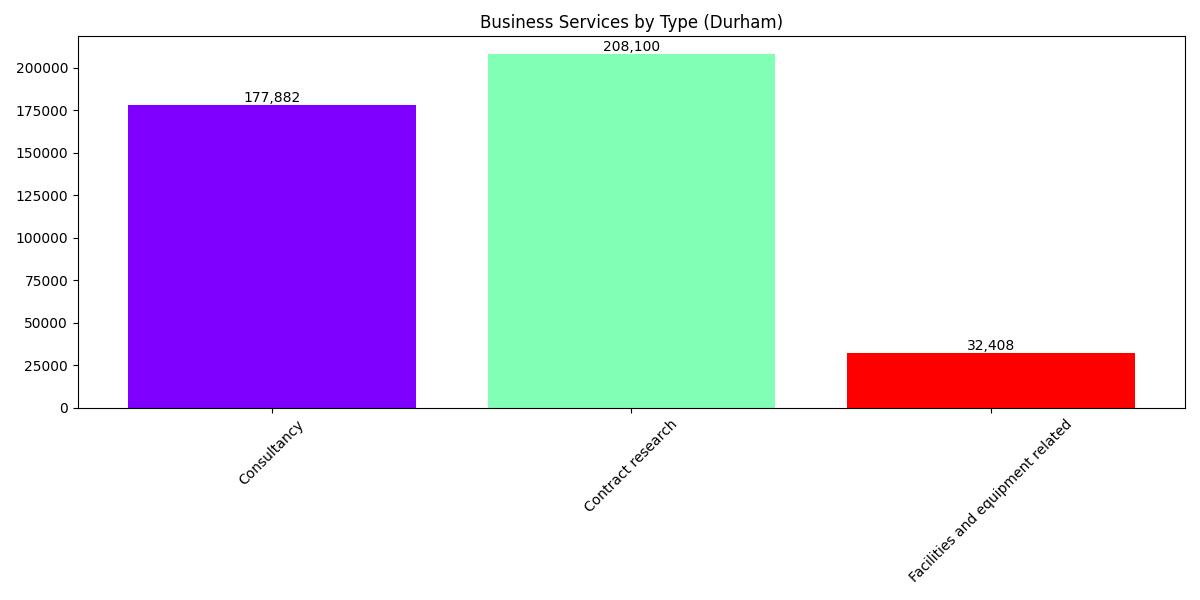
\includegraphics[width=\linewidth]{Fig/figure7.services_type.png}
        \caption{Services Type}
        \label{fig:services-type}
    \end{subfigure}
    \hfill
    \begin{subfigure}[b]{0.48\textwidth}
        \centering
        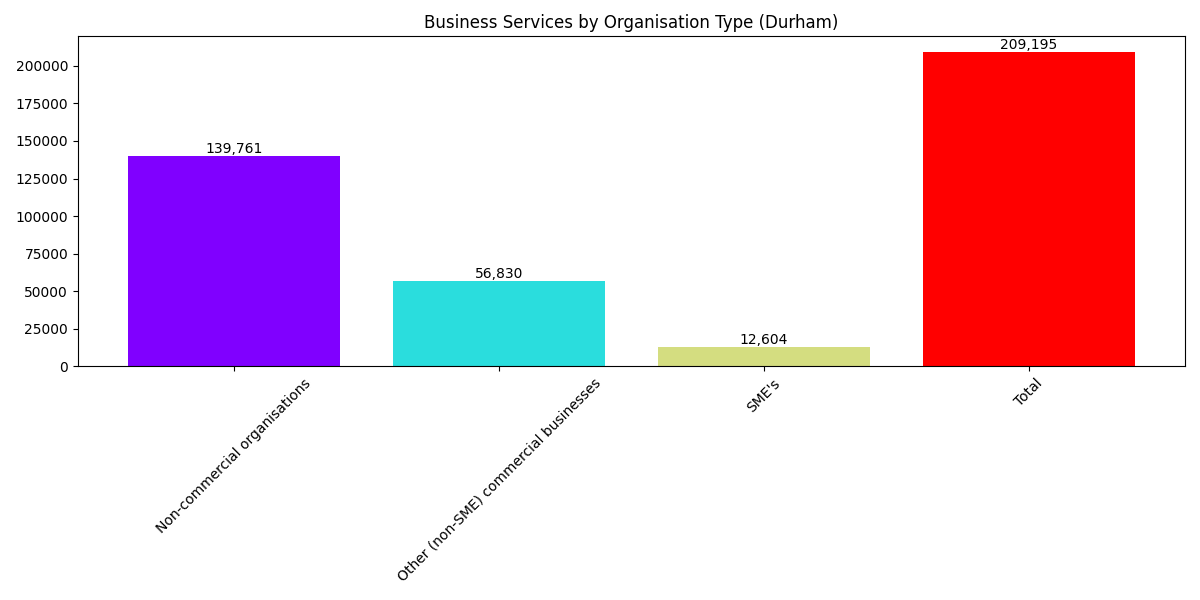
\includegraphics[width=\linewidth]{Fig/figure8.services_org_type.png}
        \caption{Services Organization Type}
        \label{fig:services-org-type}
    \end{subfigure}
    \vspace{0.6cm}
    \caption{Business Services Analysis}
    \label{fig:business-services-analysis}
\end{figure}

\begin{figure}[h]
    \centering
    \begin{subfigure}[b]{0.48\textwidth}
        \centering
        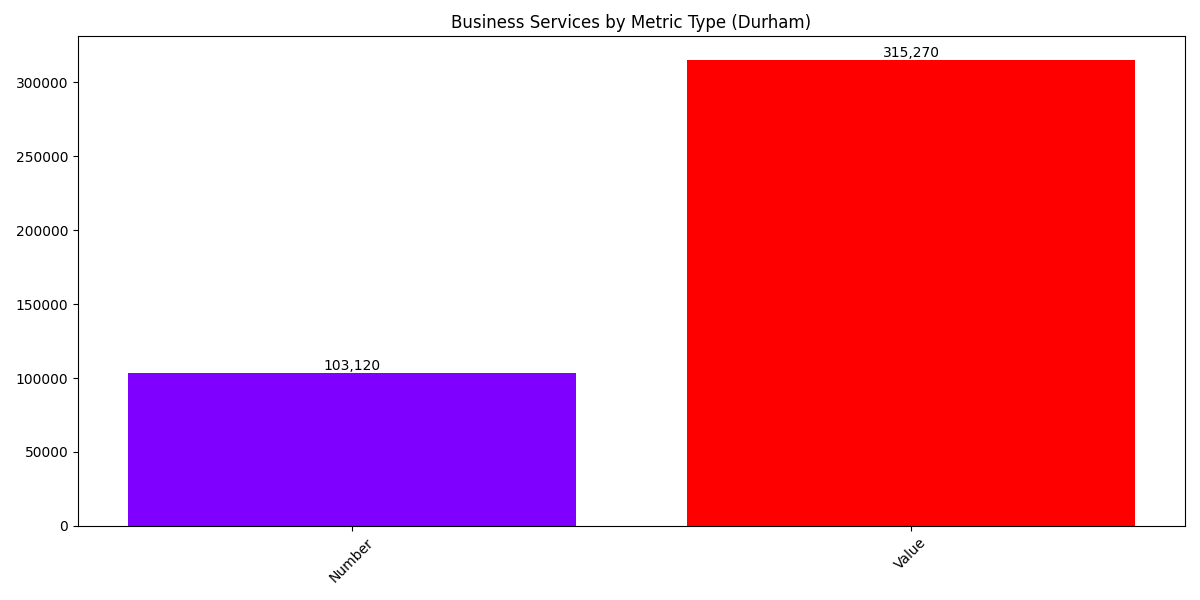
\includegraphics[width=\linewidth]{Fig/figure9.services_metric_type.png}
        \caption{Services Metric Type}
        \label{fig:services-metric-type}
    \end{subfigure}
    \hfill
    \begin{subfigure}[b]{0.48\textwidth}
        \centering
        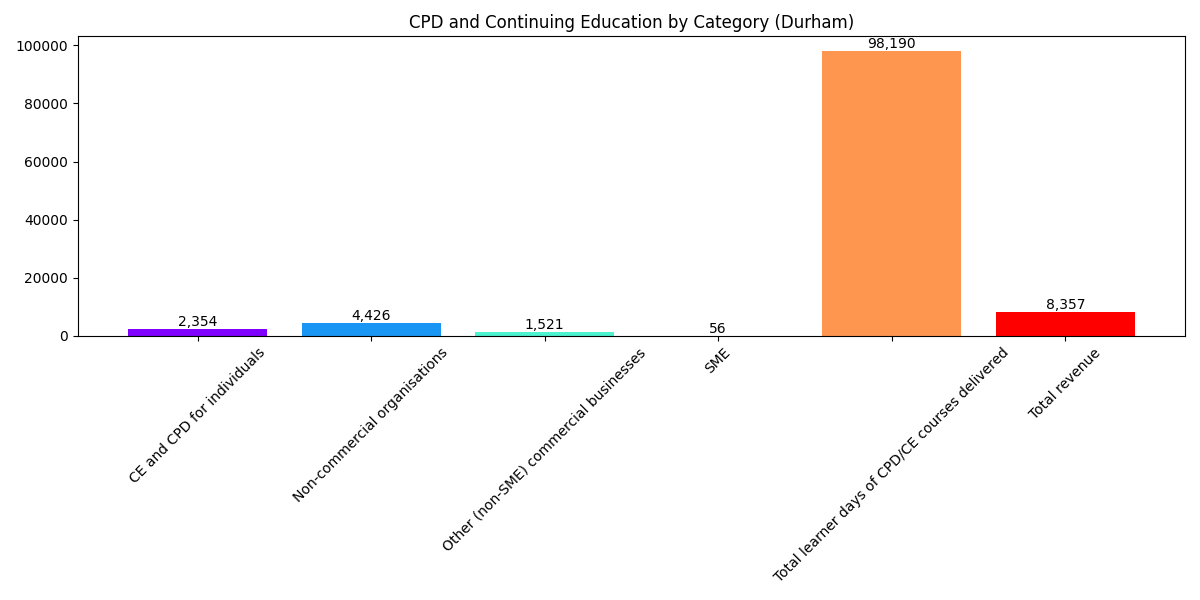
\includegraphics[width=\linewidth]{Fig/figure11.cpd_category.png}
        \caption{CPD Category}
        \label{fig:cpd-category}
    \end{subfigure}
    \vspace{0.6cm}
    \caption{Additional Services and CPD Analysis}
    \label{fig:additional-services-cpd}
\end{figure}

\begin{figure}[h]
    \centering
    \begin{subfigure}[b]{0.48\textwidth}
        \centering
        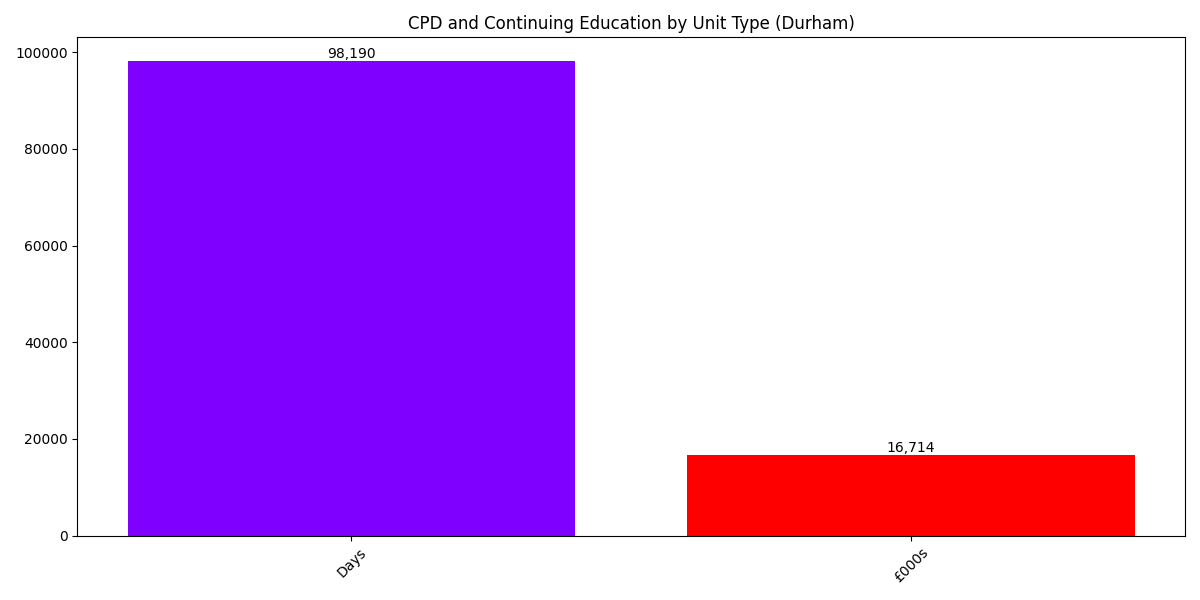
\includegraphics[width=\linewidth]{Fig/figure12.cpd_unit_type.png}
        \caption{CPD Unit Type}
        \label{fig:cpd-unit-type}
    \end{subfigure}
    \hfill
    \begin{subfigure}[b]{0.48\textwidth}
        \centering
        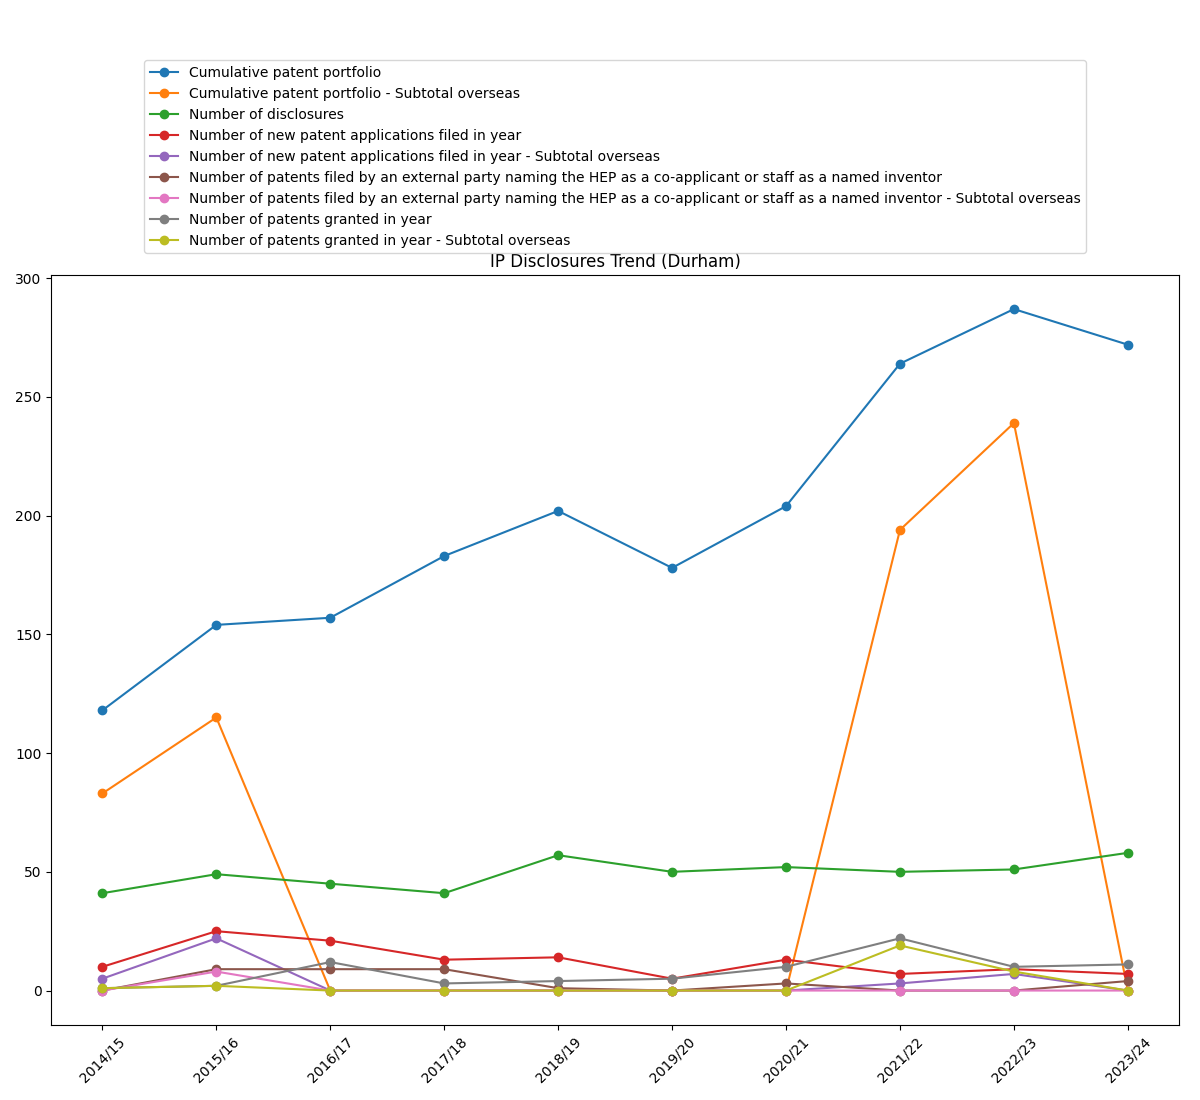
\includegraphics[width=\linewidth]{Fig/figure19.ip_disclosure_trend.png}
        \caption{IP Disclosure Trend}
        \label{fig:ip-disclosure-trend}
    \end{subfigure}
    \vspace{0.6cm}
    \caption{CPD and IP Trend Analysis}
    \label{fig:cpd-ip-trend}
\end{figure}

\begin{figure}[h]
    \centering
    \begin{subfigure}[b]{0.48\textwidth}
        \centering
        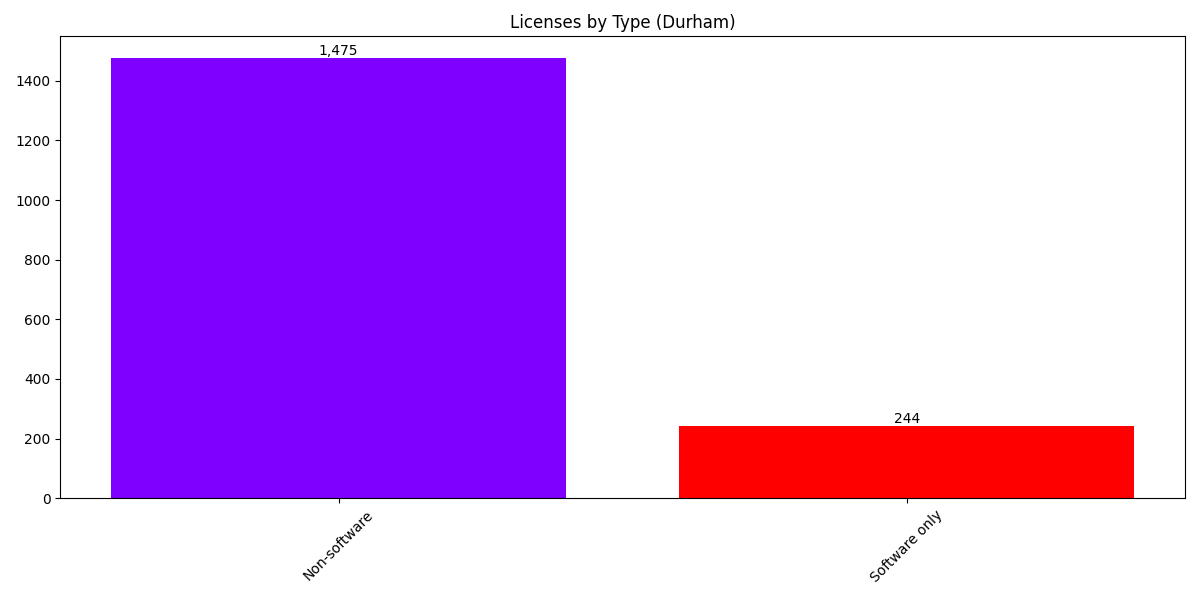
\includegraphics[width=\linewidth]{Fig/figure21.license_type.png}
        \caption{License Type}
        \label{fig:license-type}
    \end{subfigure}
    \hfill
    \begin{subfigure}[b]{0.48\textwidth}
        \centering
        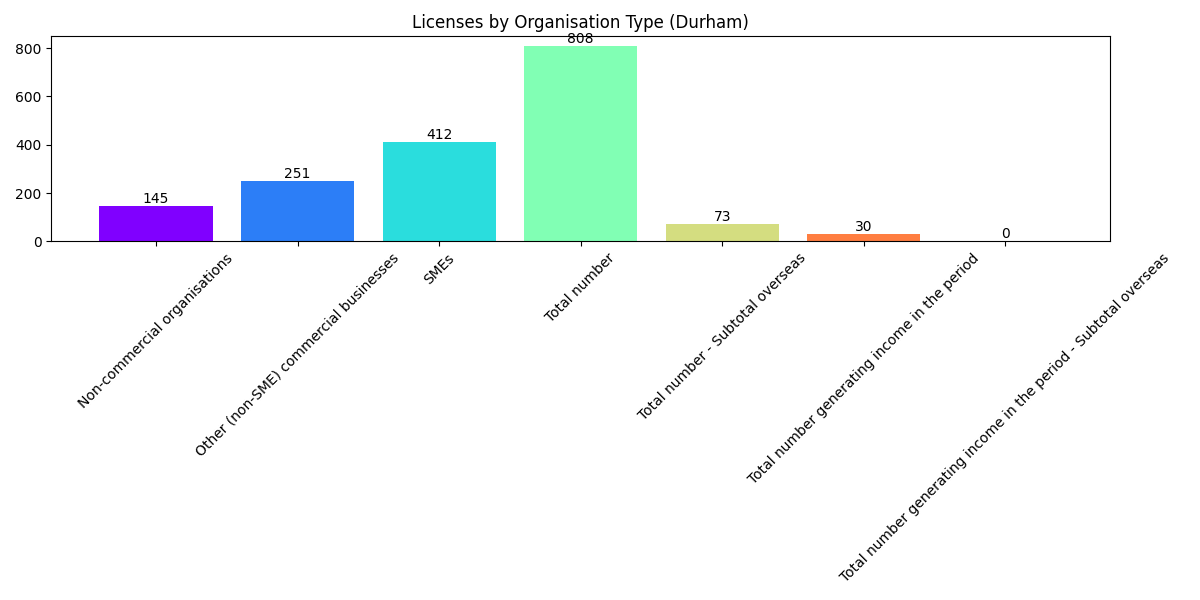
\includegraphics[width=\linewidth]{Fig/figure22.license_org_type.png}
        \caption{License Organization Type}
        \label{fig:license-org-type}
    \end{subfigure}
    \vspace{0.6cm}
    \caption{License Analysis}
    \label{fig:license-analysis}
\end{figure}

\begin{figure}[h]
    \centering
    \begin{subfigure}[b]{0.48\textwidth}
        \centering
        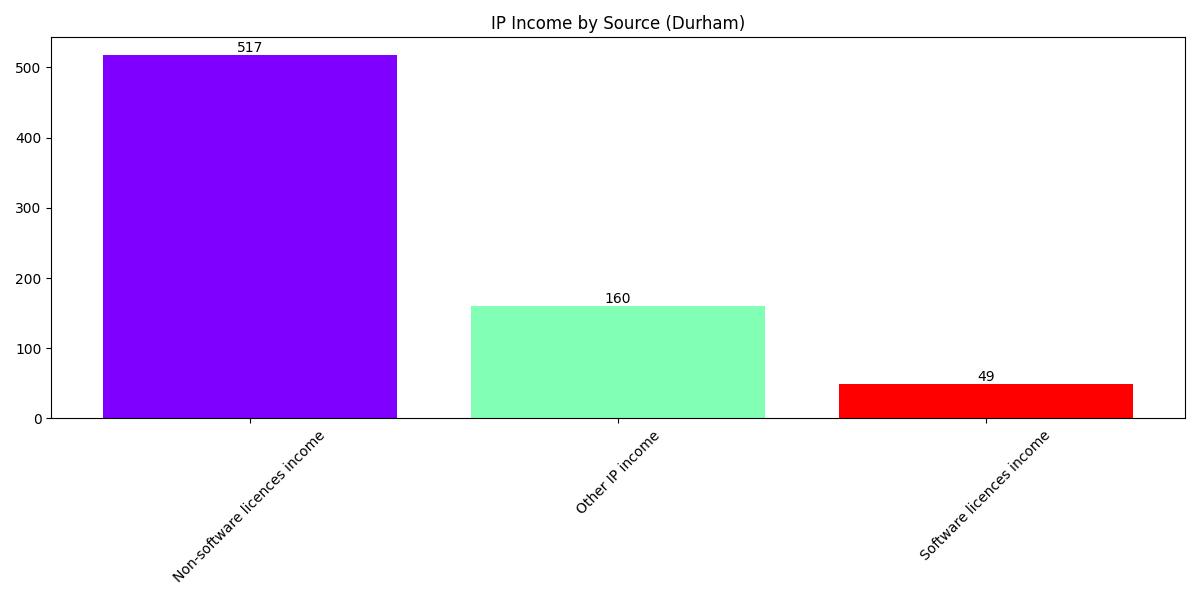
\includegraphics[width=\linewidth]{Fig/figure24.ip_income_source.png}
        \caption{IP Income Source}
        \label{fig:ip-income-source}
    \end{subfigure}
    \hfill
    \begin{subfigure}[b]{0.48\textwidth}
        \centering
        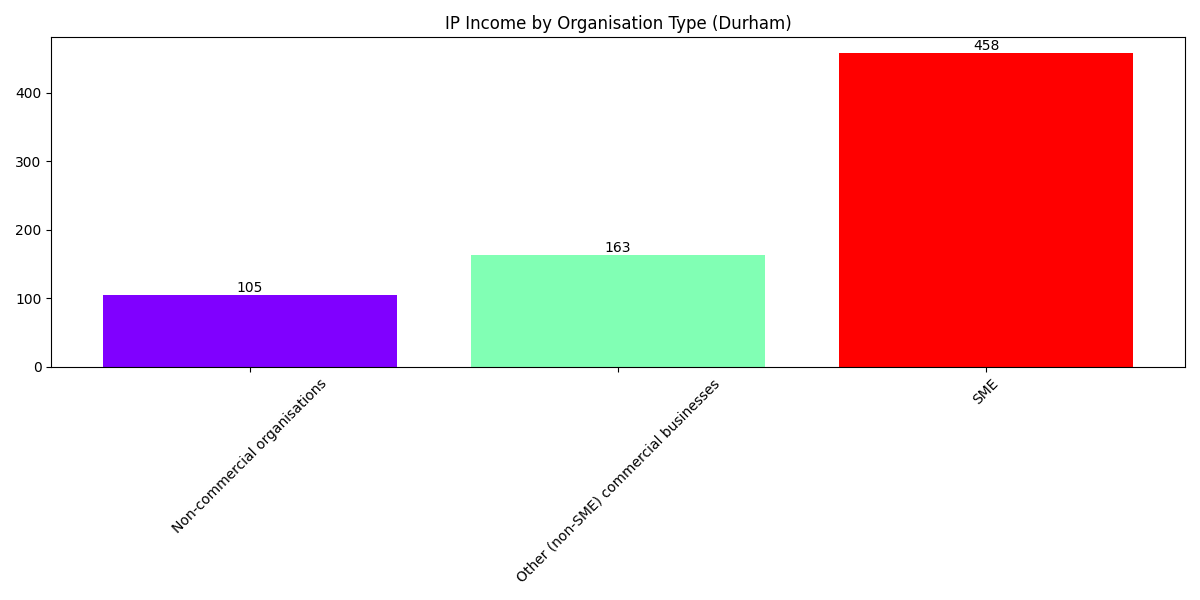
\includegraphics[width=\linewidth]{Fig/figure25.ip_income_org_type.png}
        \caption{IP Income Organization Type}
        \label{fig:ip-income-org-type}
    \end{subfigure}
    \vspace{0.6cm}
    \caption{IP Income Analysis}
    \label{fig:ip-income-analysis}
\end{figure}

\begin{figure}[h]
    \centering
    \begin{subfigure}[b]{0.48\textwidth}
        \centering
        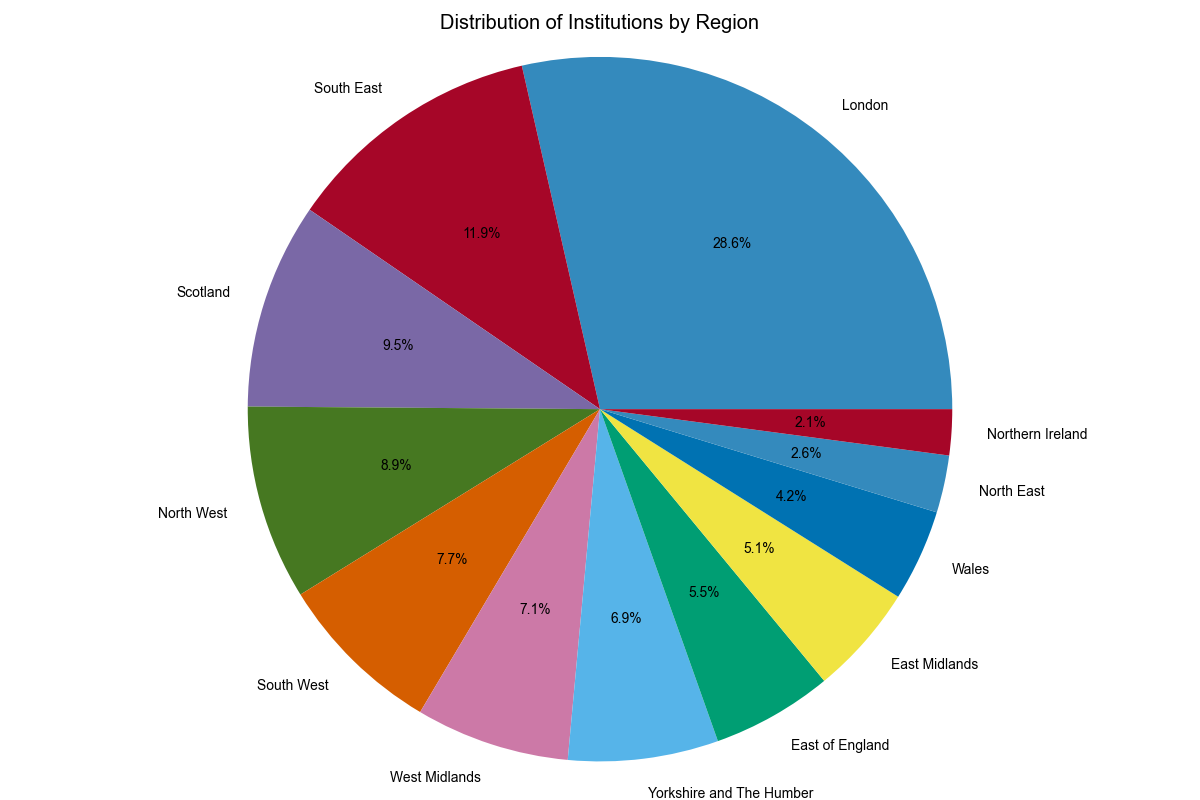
\includegraphics[width=\linewidth]{Fig/figure45.regional_distribution_pie.png}
        \caption{Regional Distribution}
        \label{fig:regional-distribution}
    \end{subfigure}
    \hfill
    \begin{subfigure}[b]{0.48\textwidth}
        \centering
        \includegraphics[width=\linewidth]{Fig/figure46.dataset_overview.png}
        \caption{Dataset Overview}
        \label{fig:dataset-overview}
    \end{subfigure}
    \vspace{0.6cm}
    \caption{Regional and Dataset Analysis}
    \label{fig:regional-dataset}
\end{figure}




\clearpage
\bibliographystyle{IEEEtran}
\bibliography{IEEEabrv, ref}

\end{document}